% % % % % % % % % % % % % % % % % % % % % % % % % % % % % % % % % % % % % % % % % % % %
%                                                                                     %
% Short Sectioned Assignment LaTeX Template Version 1.0 (5/5/12)                      %
% This template has been downloaded from: http://www.LaTeXTemplates.com               %
%                                                                                     %
% Original author:  Frits Wenneker (http://www.howtotex.com)                          %
%                                                                                     %
% Modified by: Fco Javier Sueza Rodríguez (fcosueza@disroot.org)                      %
%                                                                                     %
% Changes:                                                                            %
%	    - Custom Chapters, Sections and Subsections (titlesec package)                %
%           - Document type scrbook (oneside)                                         %
%           - Use babel-lang-spanish package and marvosym                             %
%           - Use hyperref, enumitem, tcolorbox and glossaries packages               %
%           - Use Time New Roman (mathptmx), Helvetic and Courier fonts               %
%                                                                                     %
% License: CC BY-NC-SA 3.0 (http://creativecommons.org/licenses/by-nc-sa/3.0/)        %
%                                                                                     %
% % % % % % % % % % % % % % % % % % % % % % % % % % % % % % % % % % % % % % % % % % % %

%-----------------------------------------------%
%	              Packages                  %
%-----------------------------------------------%

\documentclass[paper=a4, fontsize=11pt, oneside]{scrbook}

% ---- Text Input/Output ----- %

\usepackage[T1]{fontenc}
\usepackage[utf8]{inputenc}
\usepackage{mathptmx}
\usepackage[scaled=.92]{helvet}
\usepackage{courier}
\usepackage[indent=12pt]{parskip}

\usepackage{geometry}
\geometry{verbose,tmargin=3cm,bmargin=3cm,lmargin=2.6cm,rmargin=2.6cm}

% ---- Language ----- %

\usepackage[spanish]{babel}
\usepackage{marvosym}

% ---- Another packages ---- %

\usepackage{amsmath,amsfonts,amsthm}
\usepackage{graphics,graphicx}
\usepackage{titlesec}
\usepackage{fancyhdr}
\usepackage{tcolorbox}
\usepackage{hyperref}
\usepackage{enumitem}
\usepackage[automake]{glossaries}

%--------------------------------------------------------------------%
%                      Customizing Document                          %
%--------------------------------------------------------------------%


% ----------- Custom Chapters, Sections and Subsections -------------- %

\titleformat{\chapter}[display]
			{\bfseries\Huge}
			{Tema \ \thechapter} {0.5ex}
			{\vspace{1ex}\centering}

\titleformat{\section}[hang]
			{\bfseries\Large}
			{\thesection}{0.5em}{}

\titleformat{\subsection}[hang]
			{\bfseries\large}
			{\thesubsection}{0.5em}{}

\titleformat{\subsubsection}[hang]
			{\bfseries\large}
			{\thesubsubsection}{0.5em}{}

\hypersetup{
    colorlinks=true,
    linkcolor=black,
    urlcolor=magenta
}

% ------------------- Custom heaaders and footers ------------------- %

\pagestyle{fancyplain}

\fancyhead[]{}
\fancyfoot[L]{}
\fancyfoot[C]{}
\fancyfoot[R]{\thepage}

\renewcommand{\headrulewidth}{0pt} % Remove header underlines
\renewcommand{\footrulewidth}{0pt} % Remove footer underlines

\setlength{\headheight}{13.6pt} % Customize the height of the header

% --------- Numbering equations, figures and tables ----------------- %

\numberwithin{equation}{section} % Number equations within sections
\numberwithin{figure}{section} % Number figures within sections
\numberwithin{table}{section} % Number tables within sections

% ------------------------ New Commands ----------------------------- %

\newcommand{\horrule}[1]{\rule{\linewidth}{#1}} % Create horizontal rule command


%----------------------------------------------------------------------------------------
%	TÍTULO Y DATOS DEL ALUMNO
%----------------------------------------------------------------------------------------

\title{
\vspace{10ex}
\normalfont \normalsize
\Huge \textbf{Tarea 5: Administración Básica del Sistema (Windows II)}
}
\author{Francisco Javier Sueza Rodríguez}
\date{\normalsize\today}

%----------------------------------------------------------------------------------------
%                                     DOCUMENTO
%----------------------------------------------------------------------------------------
\begin{document}

\maketitle

\thispagestyle{empty}

\vspace{68ex}

\begin{center}
    \begin{tabular}{l l}
        \textbf{Centro}: & IES Aguadulce \\
        \textbf{Ciclo Formativo}: & Desarrollo Aplicaciones Web (Distancia)\\
        \textbf{Asignatura}: & Sistemas Informáticos\\
        \textbf{Tema}: & Tema 5 -  Administración Básica del Sistema (Windows II)\\
    \end{tabular}
\end{center}

\newpage

\tableofcontents

\newpage

\listoffigures

\newpage

\section{Caso Práctico}
María ya tiene instalado en los equipos de la empresa AguadulSoft el sistema operativo y ahora es el momento de empezar a administrar el sistema para configurarlo y ponerlo en marcha para su utilización. Como es la primera vez, Juan le va a ayudar en el proceso de administración básica del sistema. Ada será la que les dé el visto bueno.

\section{Actividades}

\subsection{Actividad 1: Estructura Departamental}
\subsubsection{Enunciado}

Crea la siguiente estructura departamental de carpetas colgando directamente de la raíz del disco en la que está instalado Windows 10. Crea primero la carpeta "AguadulSoft" y dentro de esta las demás:

    \begin{figure}[H]
    \centering
    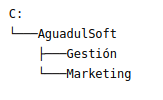
\includegraphics[scale=0.80]{estructura-enunciado.png}
    \caption{Estructura de carpetas a crear}
\end{figure}

Introduce dos archivos, un documento y una imagen, en la carpeta de cada departamento (Gestión y Marketing) y nómbralos como tipoArchivo\_nombreDepartamento (por ejemplo, en la carpeta ``Gestión'' el documento sería nombrado como ``documento\_gestión'' y la imagen como ``imagen\_gestión'').

\textbf{Capturas}:

\begin{itemize}
    \item Muestra de la estructura departamental de carpetas y de su ubicación.
    \item Archivos de cada carpeta.
\end{itemize}

\subsubsection{Solución}
\begin{enumerate}
    \item En primer lugar hemos creado los directorios desde la interfaz gráfica.

    \begin{figure}[H]
        \centering
        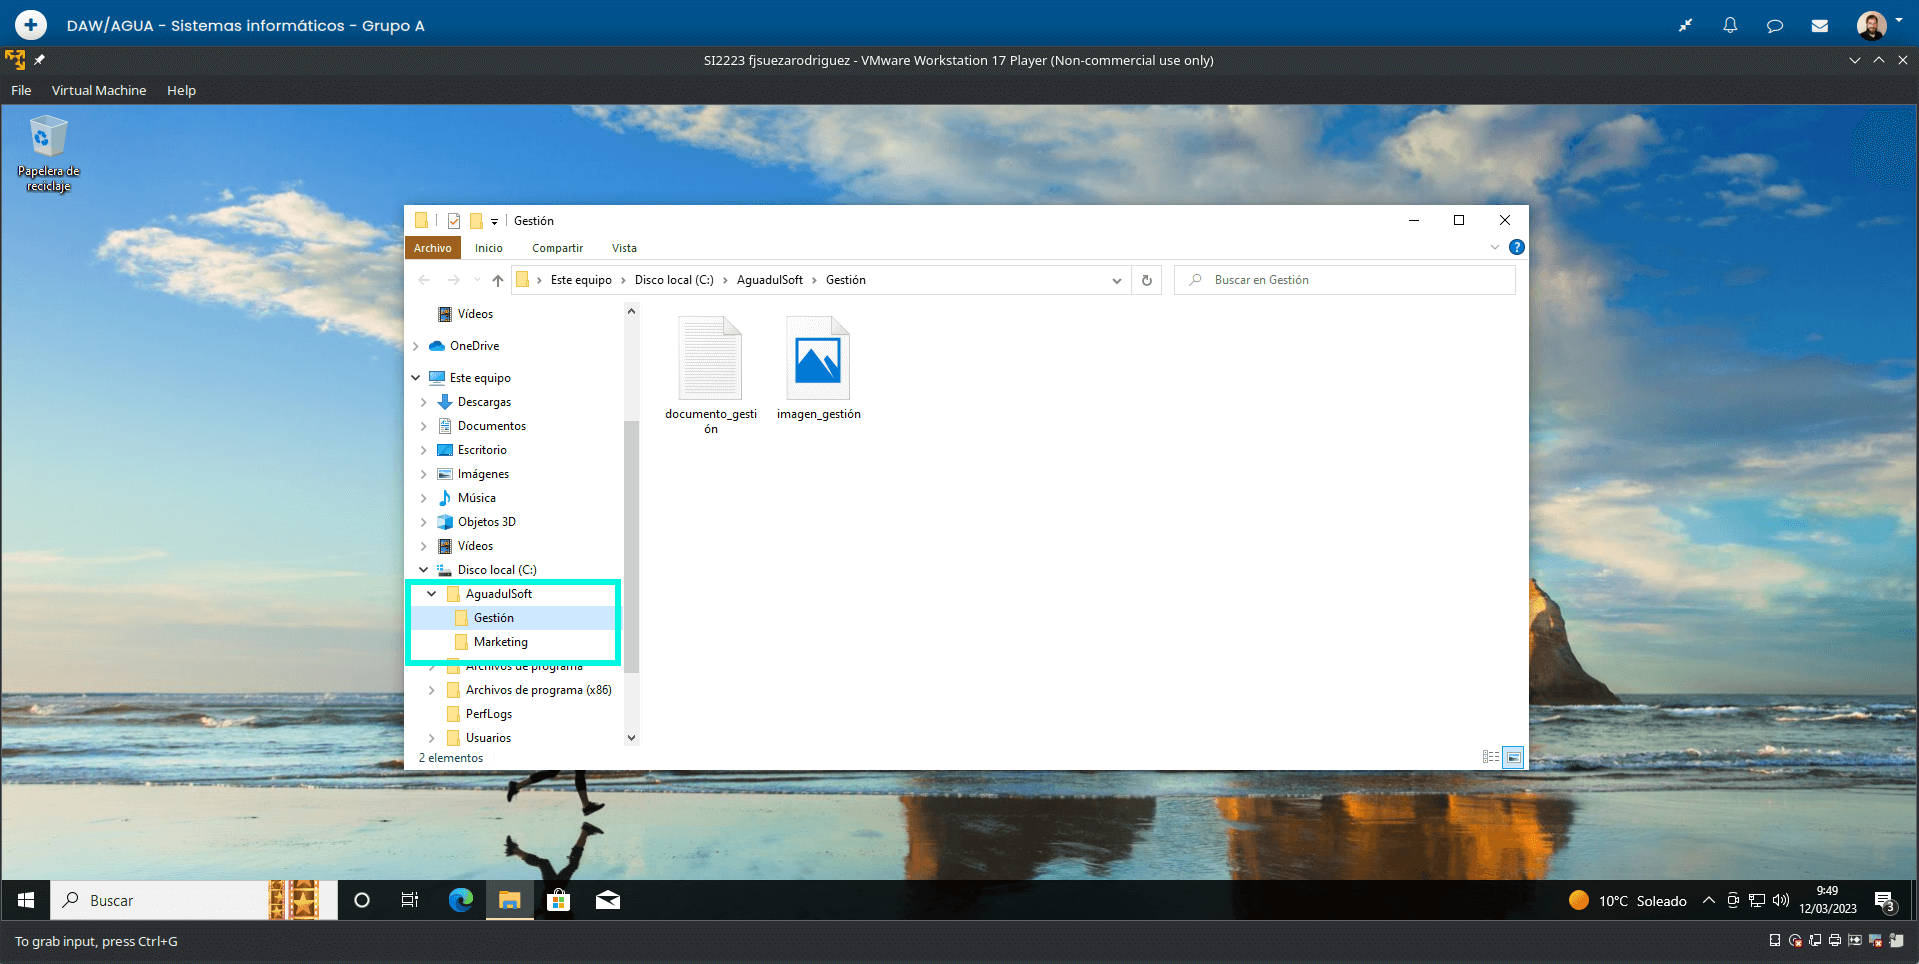
\includegraphics[scale=0.14]{estructura.png}
        \caption{Estructura de directorios creada}
    \end{figure}

    \item A continuación, hemos añadido 2 archivos a cada directorio creado, como se especifica en el enunciado. Se ha usado también la opción ``\textbf{Nuevo ---> archivo de texto/imagen de mapa de bits}'' para crear estos archivos.

    \begin{figure}[H]
        \centering
        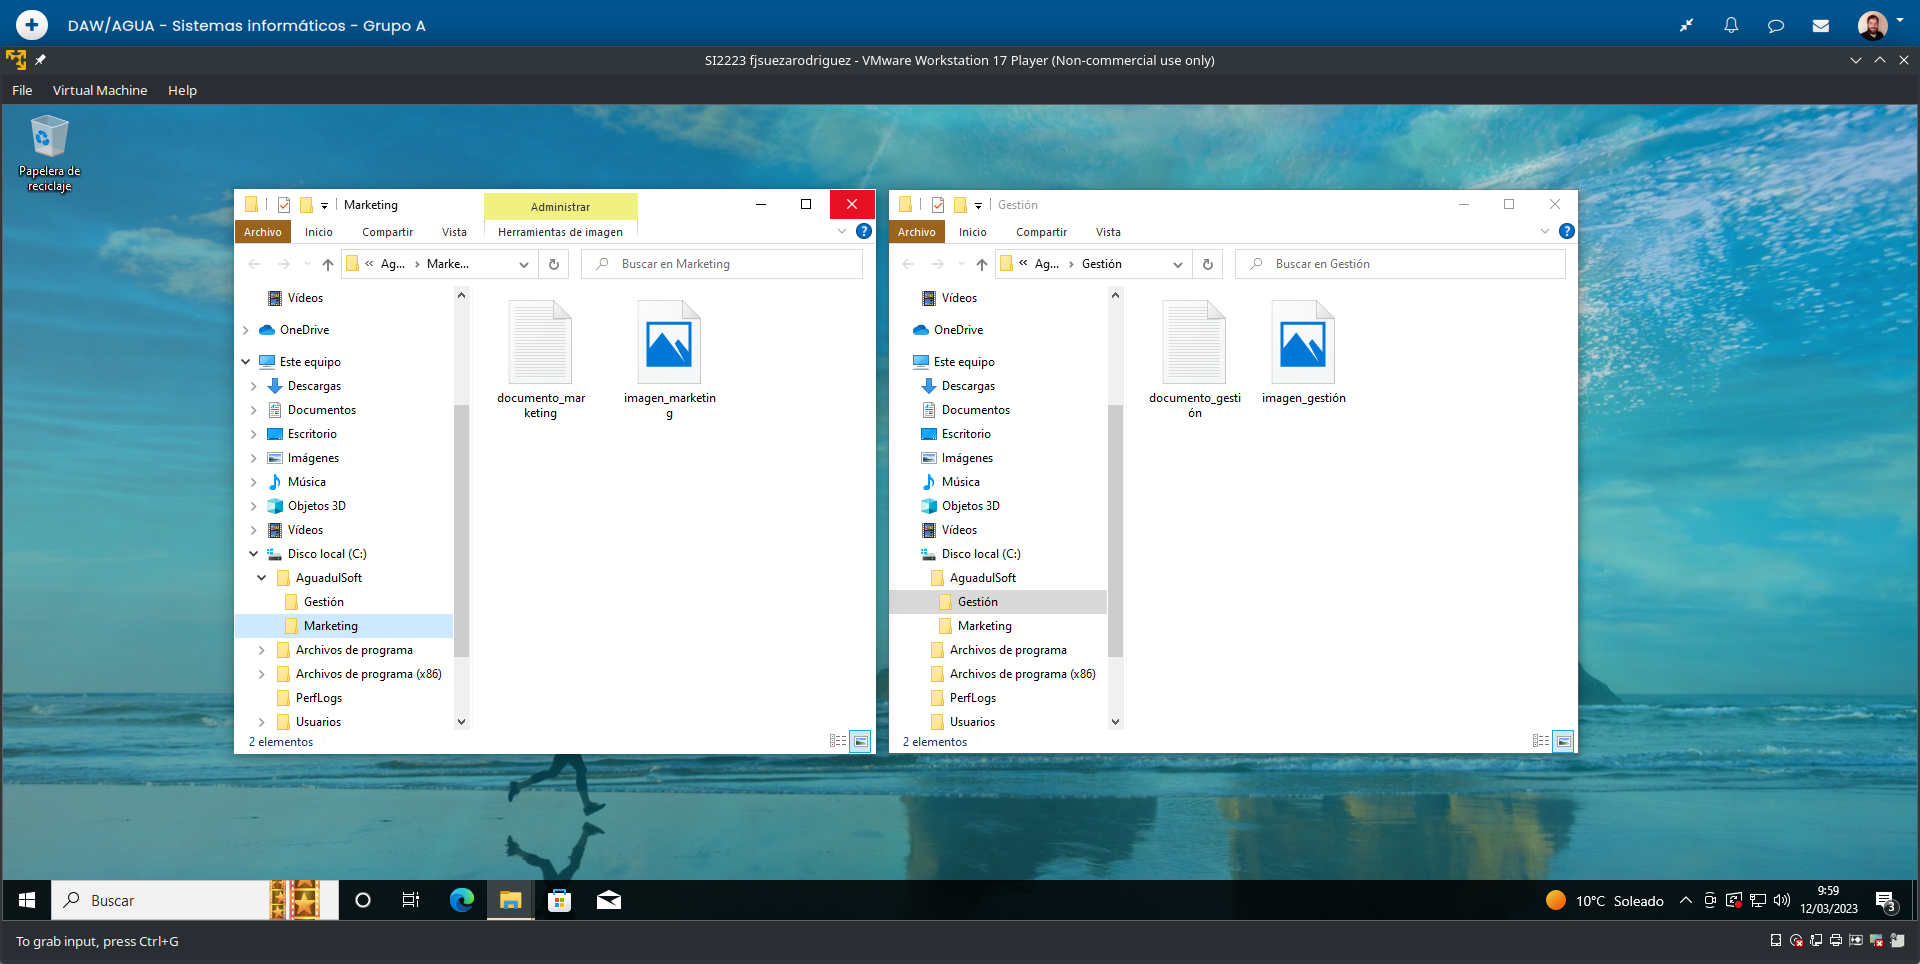
\includegraphics[scale=0.18]{estructura-archivos.png}
        \caption{Archivos creados es las carpetas Marketing y Gestión}
    \end{figure}
\end{enumerate}

\subsection{Actividad 2: Cuentas de Usuario Locales}

\subsubsection{Enunciado}

\begin{enumerate}[label=2.\alph*)]
    \item \textbf{Creación de Usuarios}: crea las siguientes cuentas de usuarios locales (con privilegios limitados):
    \begin{itemize}
        \item Gestión: Graciela Góngora y Genaro García.
        \item Marketing: Matías Martínez y Marta Mejías.
    \end{itemize}

    Nombra cada cuenta de usuario como InicialNombreApellido e introduce en el campo ``Nombre completo'' su nombre y apellido completos y en el campo ``Descripción'' el nombre del departamento al que pertenece (por ejemplo, el usuario ``Graciela Góngora'' del departamento ``Gestión'' sería nombrado como ``ggongora'' y en sus campos se introduciría ``Graciela Góngora'' en ``Nombre completo'' y ``Dpto. de Gestión'' en ``Descripción'').

    \textbf{Capturas}:
    \begin{itemize}
        \item Ventana/consola donde se crea un nuevo usuario (indica textualmente cómo se accede a dicha ventana).
        \item Introducción del nombre y campos "Nombre completo" y "Descripción" de la primera cuenta de usuario.
        \item Resumen de las cuentas de usuario creadas con sus respectivos nombres yitemize
    \end{itemize}

    \item \textbf{Creación de Grupos}: crea un grupo de usuarios para cada departamento, nómbralos con su nombre de departamento y en el campo ``Descripción'' introduce el texto ``Departamento de X'' donde X es el nombre del departamento (por ejemplo, el grupo de usuarios del departamento ``Gestión'' sería nombrado como ``Gestión'' y en su campo ``Descripción'' se introduciría ``Departamento de gestión'').

    Incluye en cada uno de ellos sus usuarios correspondientes, creados en la actividad anterior.

    \textbf{Capturas}:
    \begin{itemize}
        \item Ventana donde se crea un nuevo grupo de usuarios (indica textualmente cómo se accede a dicha ventana).
        \item Introducción del nombre y campo ``Descripción'' del primer grupo de usuarios.
        \item Asignación de los usuarios del primer grupo de usuarios.
        \item Resumen de los grupos de usuarios creados con sus respectivos nombres, campos y usuarios.
    \end{itemize}
\end{enumerate}

\subsubsection{Solución}

\begin{enumerate}
    \item En primer lugar, hemos \textbf{creado los usuarios solicitados} con los datos que se especifican en el enunciado. Hemos elegido la opción de crearlos mediante la aplicación \textbf{LUSRMGR.MSC}, ya que es la que proporciona la opciones de configuración más completas.

    Para acceder a esta aplicación, hemos ejecutado el comando \textbf{LUSRMGR.MSC} en consola, aunque se puede poner también en la barra de búsqueda de Windows y clickar en la aplicación que nos da como resultado. Una vez ahí, hemos pulsado en la opción ``\textbf{Acciones adicionales ---> Nuevo usuario}.

     \begin{figure}[H]
        \centering
        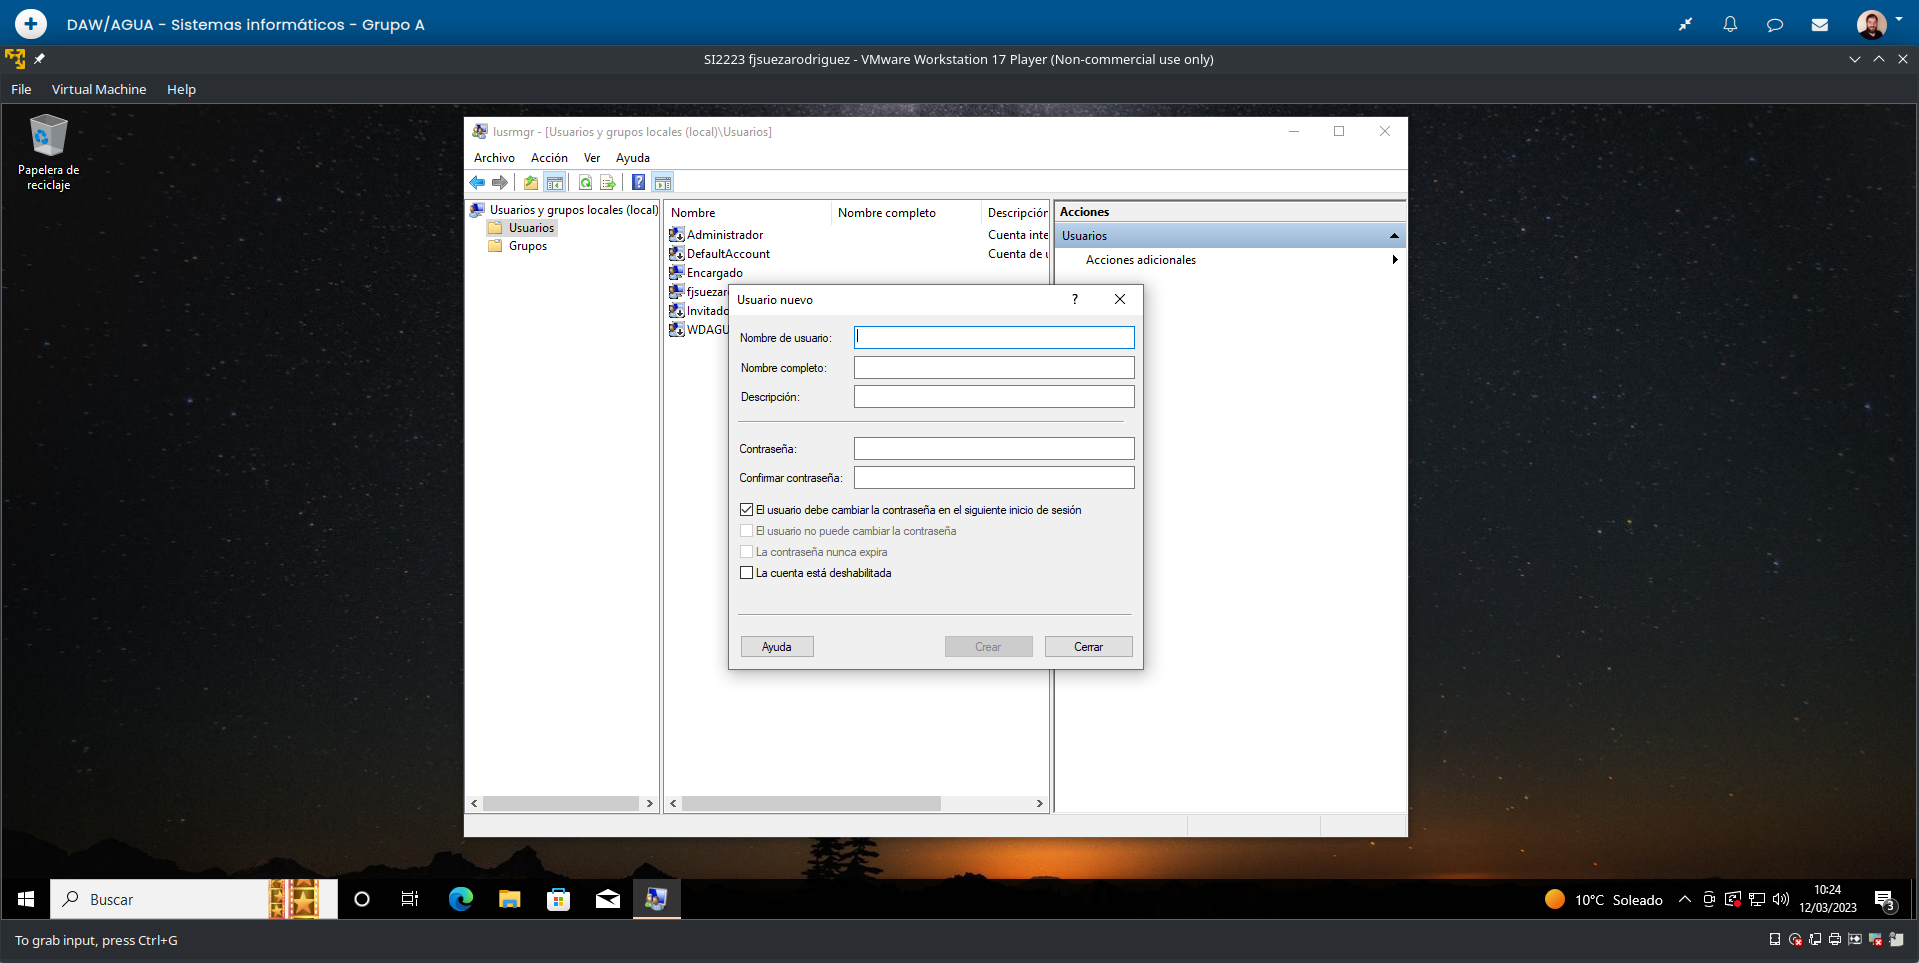
\includegraphics[scale=0.16]{usuarios-creacion.png}
        \caption{Ventana de creación de usuario}
    \end{figure}

    A continuación hemos introducido los datos solicitados, tal y como se explica en el enunciado.

    \begin{figure}[H]
        \centering
        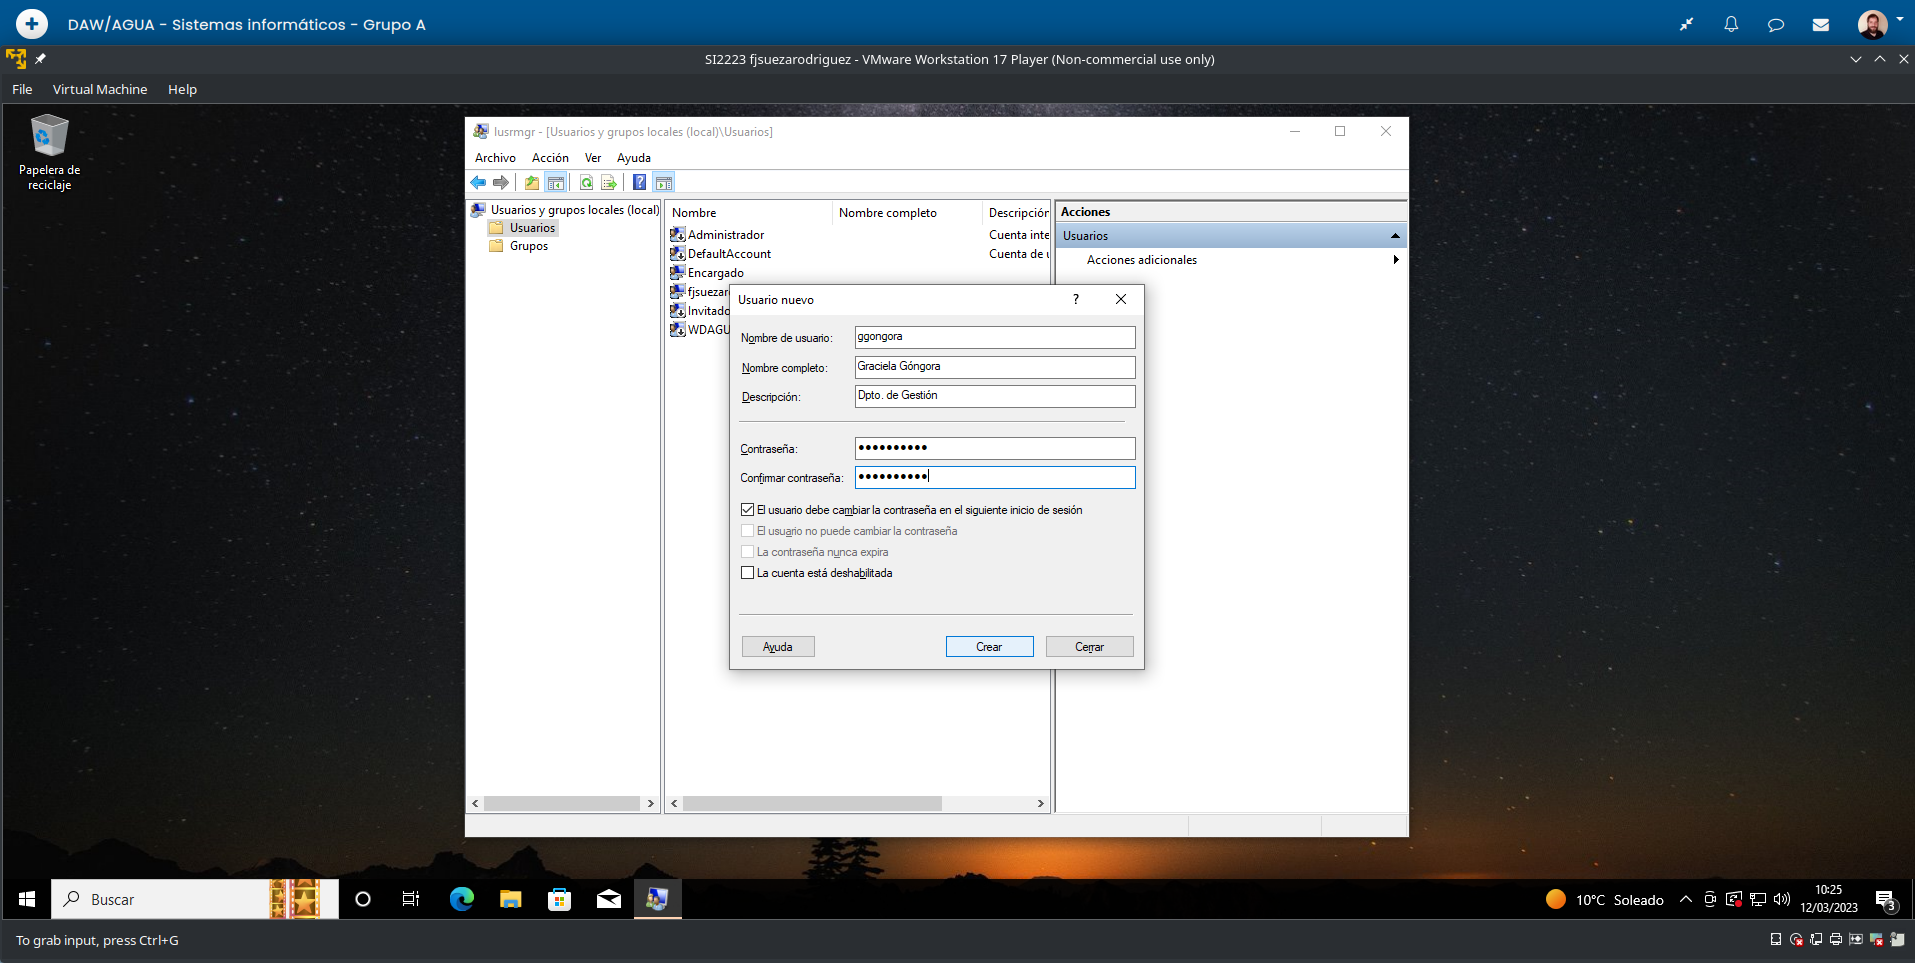
\includegraphics[scale=0.16]{usuarios-datos.png}
        \caption{Introducción de datos de usuario}
    \end{figure}

    Tras haber creado los 4 usuarios que se piden, las cuentas de usuario que tenemos en el sistema las podemos ver en la ventana principal de \textbf{lusrmgr}, como vemos en la siguiente captura.

    \begin{figure}[H]
        \centering
        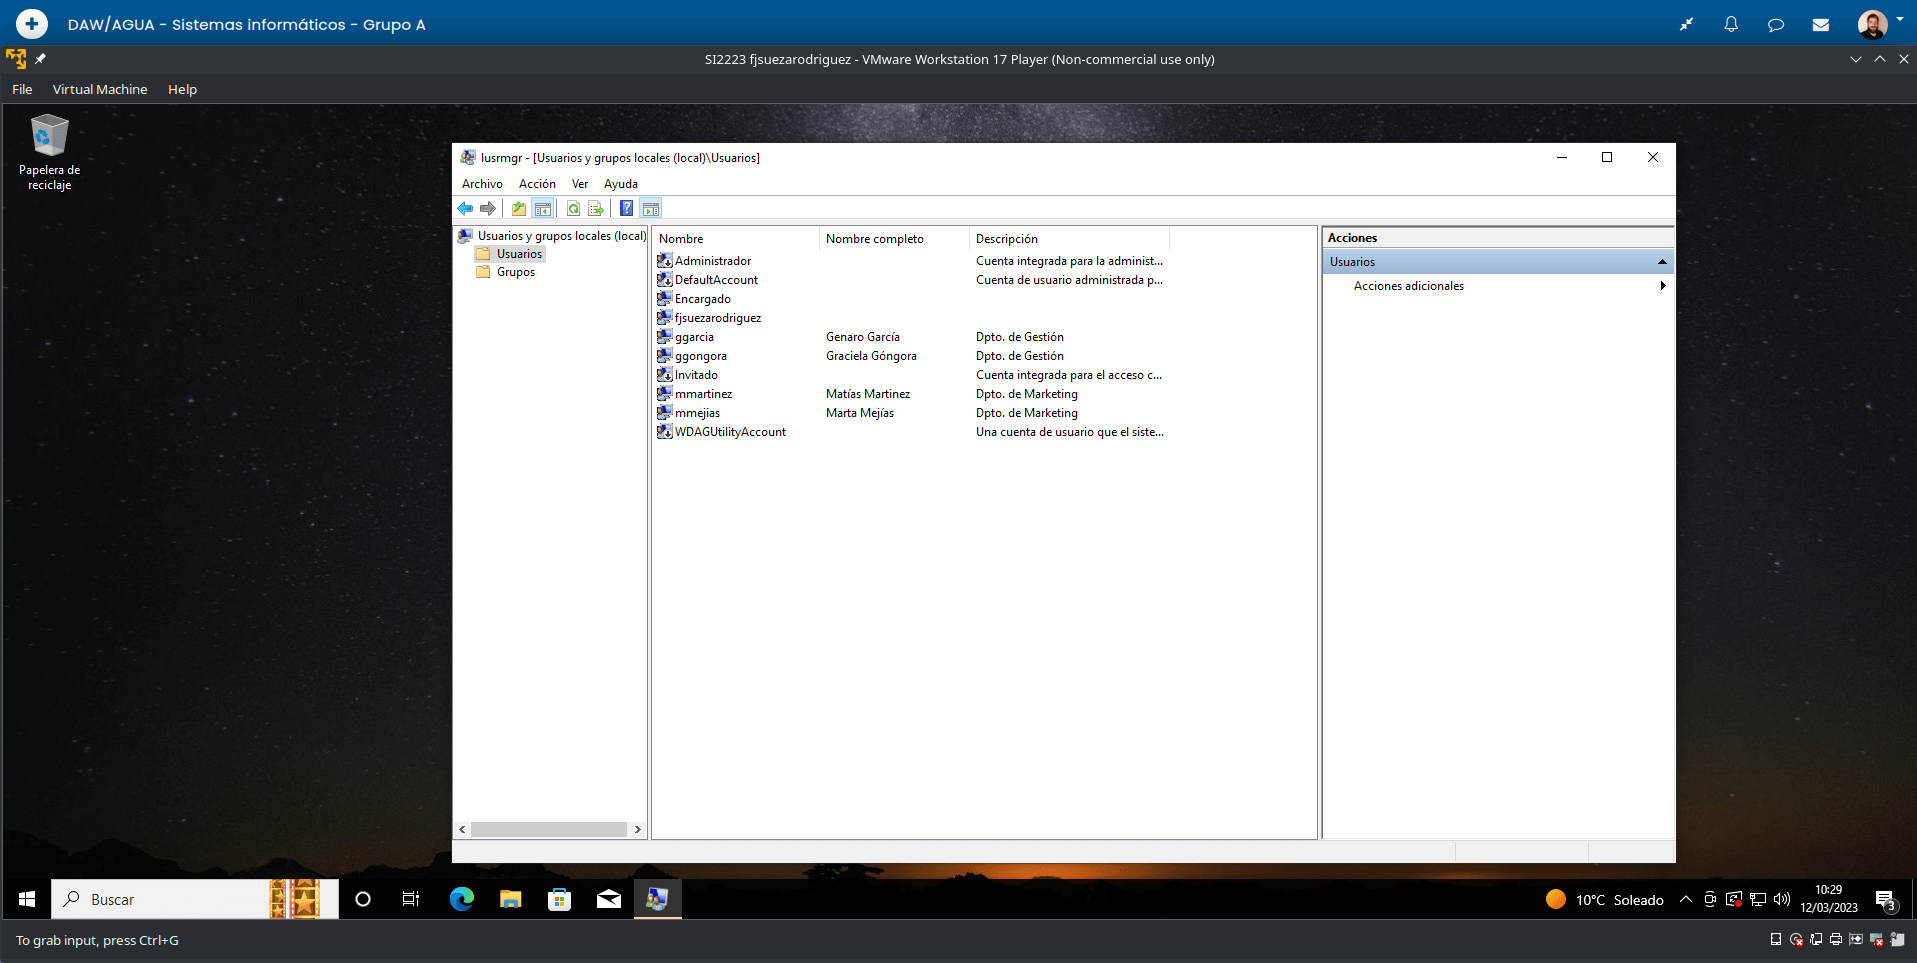
\includegraphics[scale=0.16]{usuarios-creados.png}
        \caption{Usuario creados con lusrmgr}
    \end{figure}

    \item En segundo lugar vamos a \textbf{crear los grupos} que se nos piden y añadir a ellos los usuarios pertinentes. Para esa tarea vamos a usar también la aplicación \textbf{lusrmgr}, tal y como hemos hecho en el punto anterior. La forma de acceso a la aplicación es la misma que en punto anterior, la única diferencia es que hemos pulsado en la opción \textbf{Grupos} del menú de la izquierda una vez abierta esta.

    \begin{figure}[H]
        \centering
        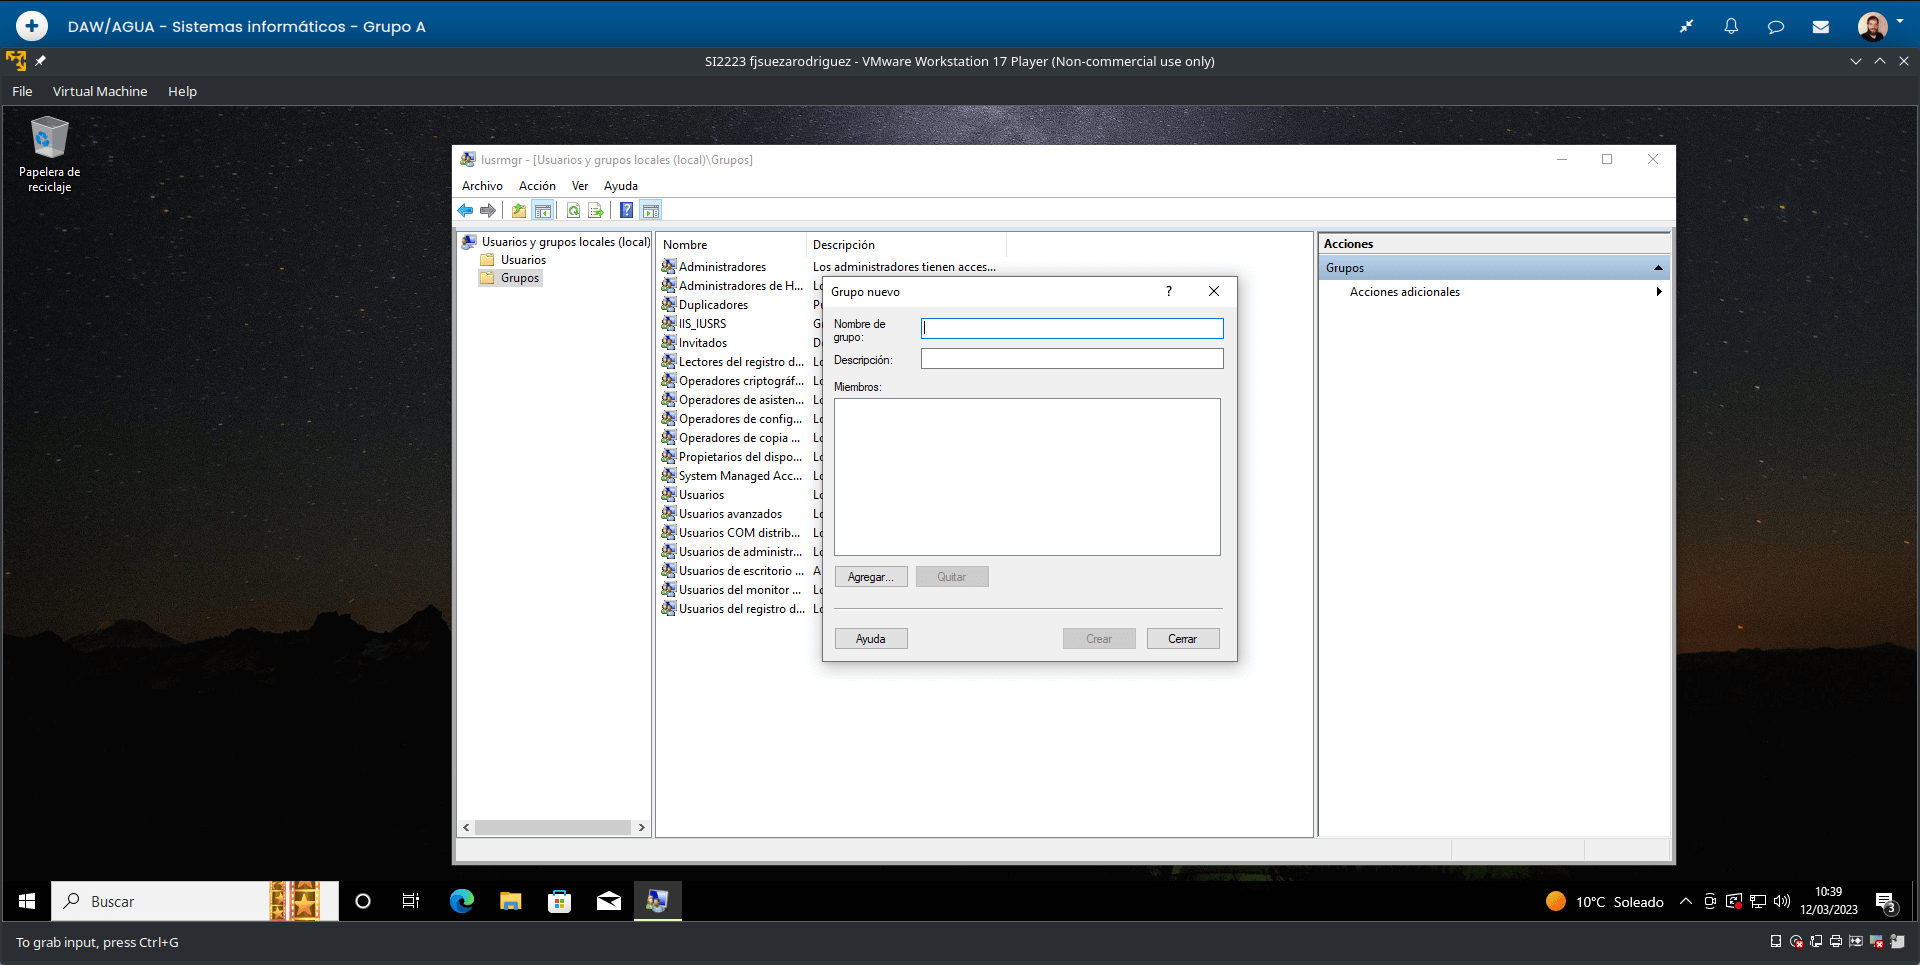
\includegraphics[scale=0.16]{grupos-creaci.png}
        \caption{Ventana de creación de un nuevo grupo}
    \end{figure}

    Una vez que estamos en esta ventana, podemos introducir los diferentes datos que se nos piden, como es el nombre del grupo y su descripción.

    \begin{figure}[H]
        \centering
        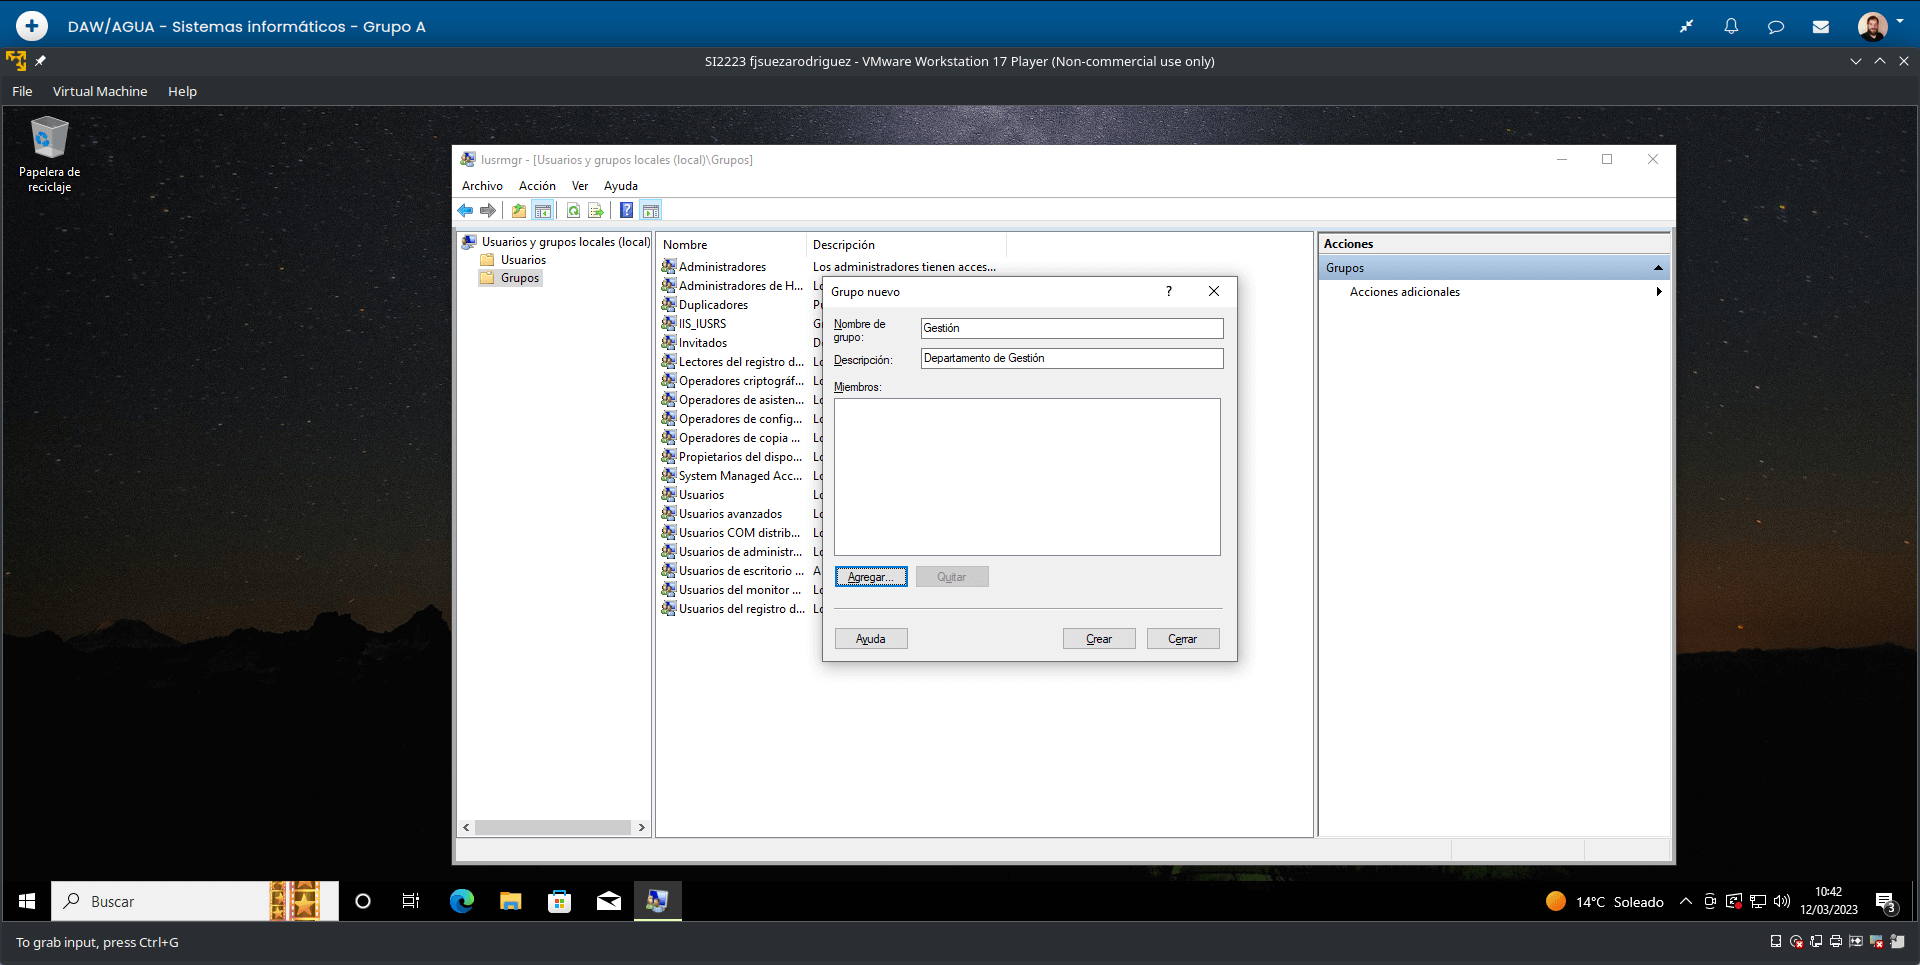
\includegraphics[scale=0.16]{grupos-datos.png}
        \caption{Introducción de datos del nuevo grupo}
    \end{figure}

    En esta misma ventana, podemos agregar los usuarios pertenecientes a dicho grupos, pulsando en el botón \textbf{Agregar} e introduciendo el nombre del usuario en cuestión.

    \begin{figure}[H]
        \centering
        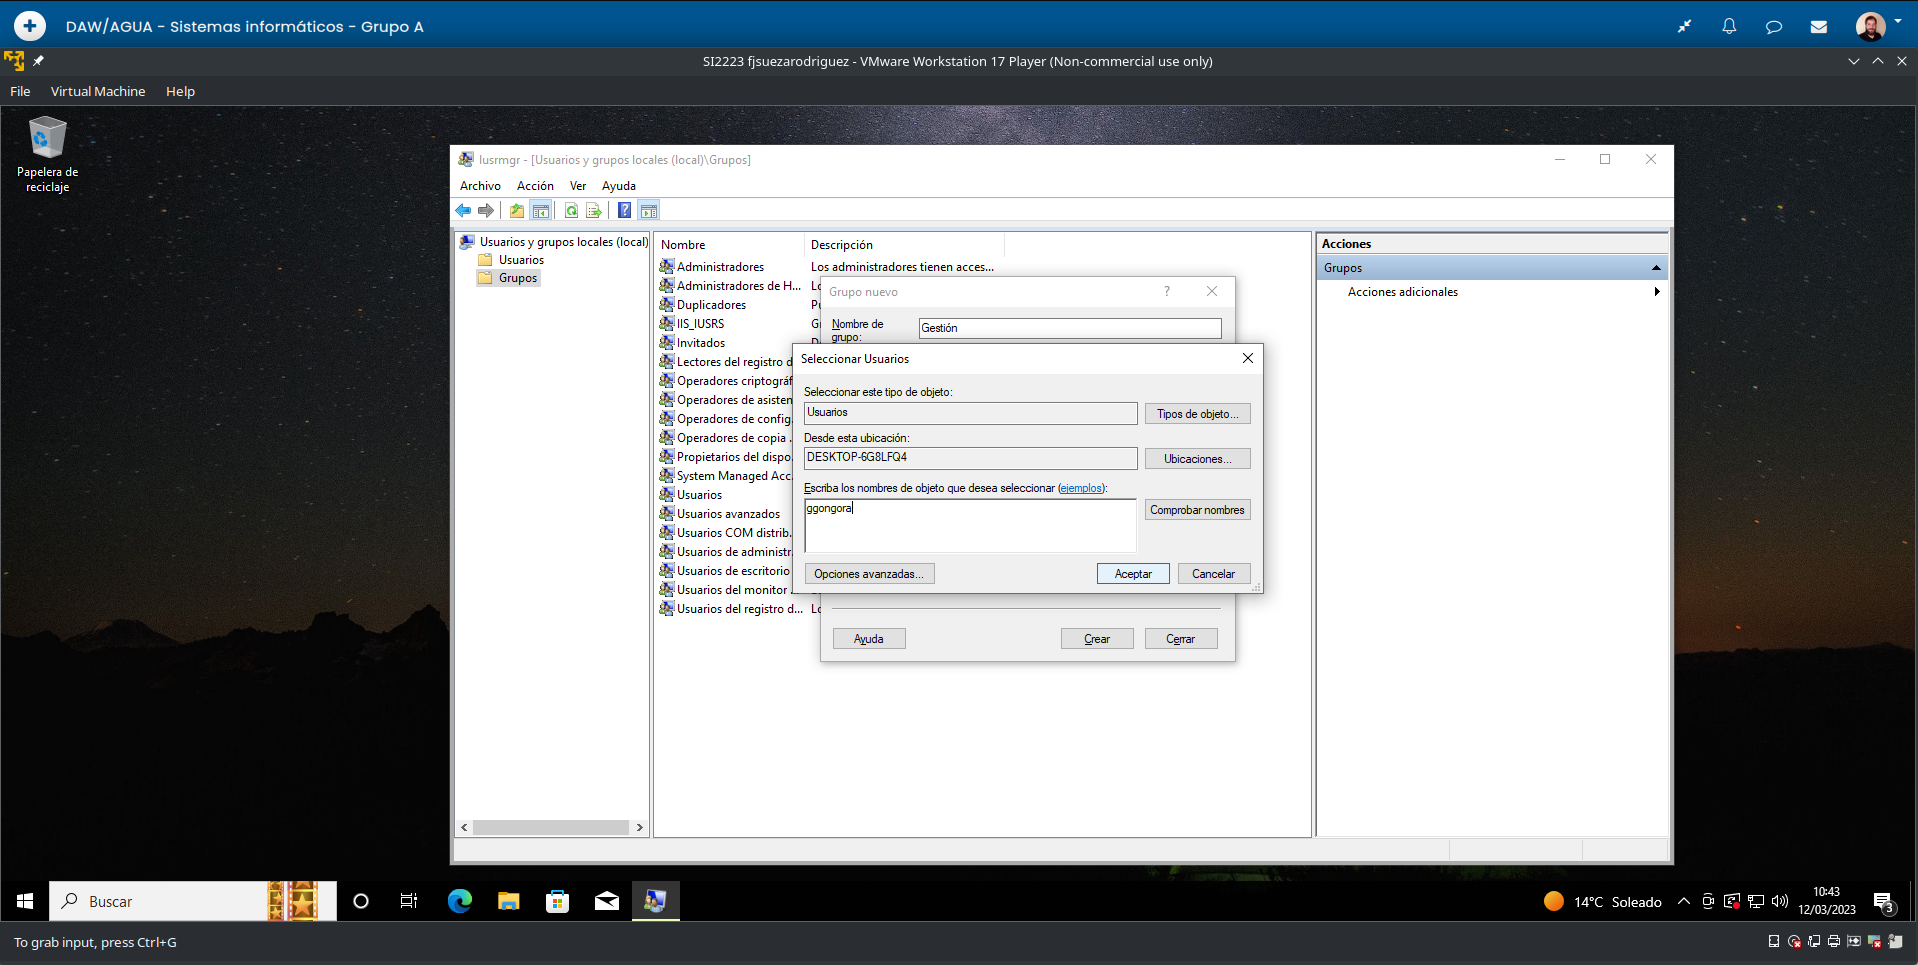
\includegraphics[scale=0.16]{grupos-usuarios.png}
        \caption{Agregación de un usuario al grupo}
    \end{figure}

    Una vez creados los dos grupos y agregados los usuarios que pertenecen a cada uno, estos han quedado como se puede ver en las siguientes dos capturas.

    \begin{figure}[H]
        \centering
        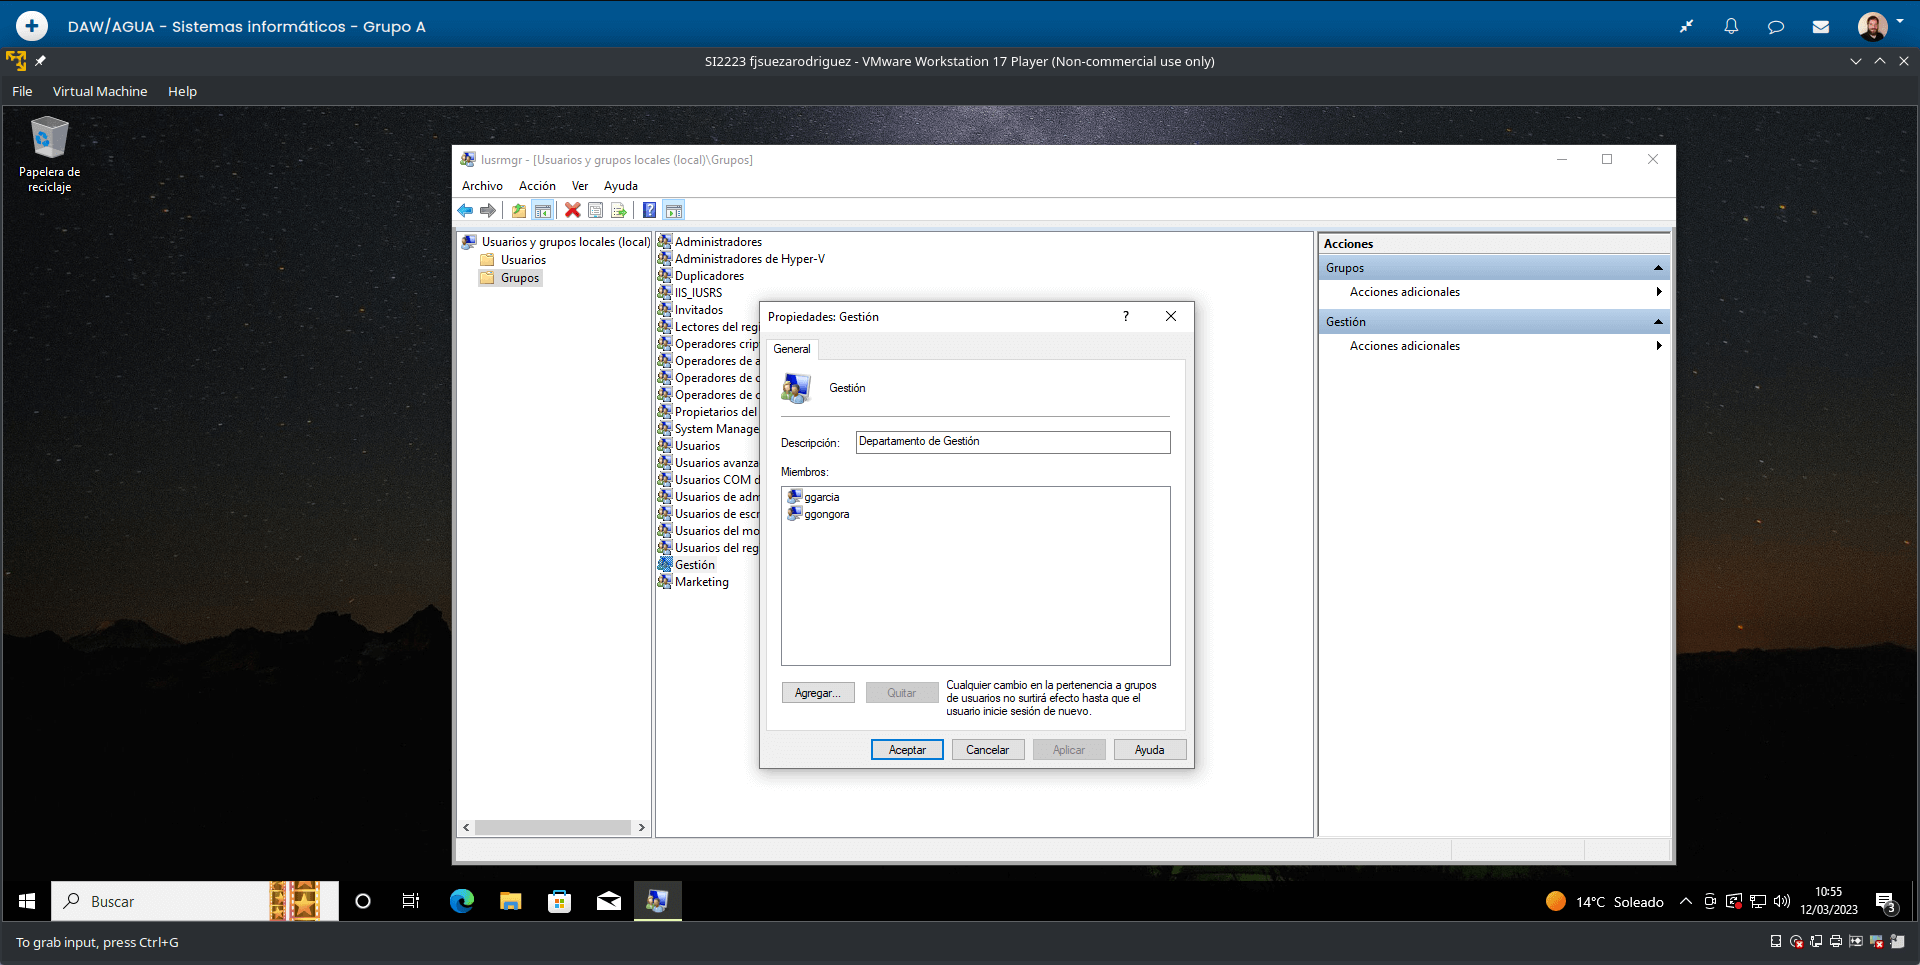
\includegraphics[scale=0.16]{grupos-gestion.png}
        \caption{Grupo Gestión creado}
    \end{figure}

    \begin{figure}[H]
        \centering
        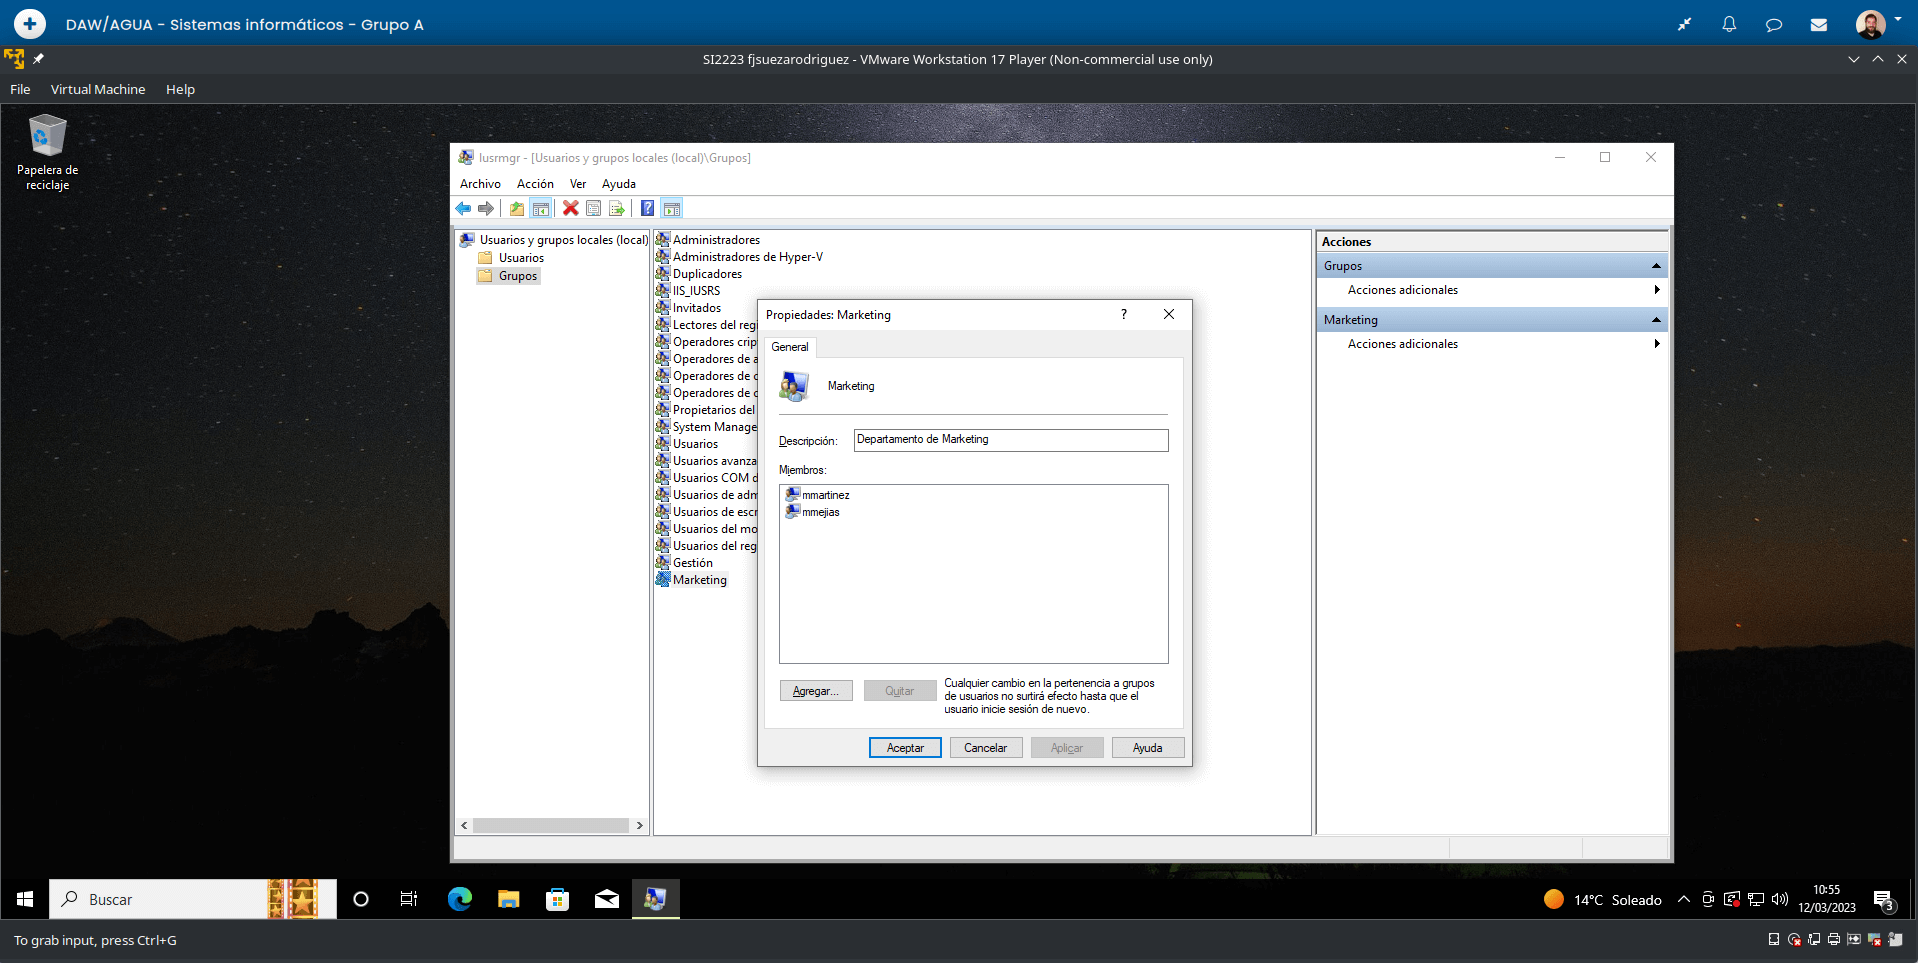
\includegraphics[scale=0.16]{grupos-marketing.png}
        \caption{Grupo Marketing creado}
    \end{figure}
\end{enumerate}

\subsection{Actividad 3: Permisos de Archivos y Carpetas}

\subsubsection{Enunciado}
Configura los permisos de las carpetas creadas en la primera actividad, para que los usuarios creados en la segunda actividad, tengan permisos de lectura y escritura sobre la carpeta de su departamento. El resto de usuarios, aunque se cree posteriormente en el sistema, no tendrá ningún acceso si no pertenece a ese departamento. Los permisos se asignarán a los grupos que creaste en la actividad 2.b, no a los usuarios de manera individual.

A continuación, para comprobar que los permisos aplicados son correctos, inicia sesión con un usuario de un departamento, intenta acceder a la carpeta de su departamento y a la del otro departamento, e indica qué ocurre en cada caso. Realiza también la comprobación de acceder con el usuario creado en la instalación de Windows 10 a las carpetas de los departamentos.

\textbf{Capturas}:

\begin{itemize}
    \item Ventana donde se asignan los permisos de la carpeta ``Gestión'' (indica textualmente cómo se accede a dicha ventana).
    \item Proceso de asignación de permisos a la carpeta ``Gestión''. Deben mostrarse los nombres de los grupos implicados sus respectivos permisos.
    \item Resumen de la asignación de permisos a la carpeta ``Marketing''. Deben mostrarse los nombres de los grupos implicados y sus respectivos permisos.
    \item Acceso de un usuario de un departamento a la carpeta de su departamento y a la del otro departamento.
    \item Acceso del usuario creado en la instalación de Windows 10 a las carpetas de los departamentos.
\end{itemize}

\subsubsection{Solución}

En esta actividad vamos a cambiar los permisos de las carpetas creadas en la Actividad 1 para que solo los usuarios pertenecientes a dichos departamentos puedan acceder a ellos y modificarlos. Para ellos hemos realizado los siguientes pasos.

\begin{enumerate}
    \item Primero hemos modificado los permisos del directorio \textbf{Gestión}. Para ello, nos hemos situado en su directorio padre, \textbf{AguadulSoft}, y hemos hecho click con el \textbf{botón derecho} sobre el directorio y pulsado en la opción \textbf{Propiedades} del menú que se nos despliega. A continuación, hemos pulsado en la pestaña \textbf{Seguridad}.

    \begin{figure}[H]
        \centering
        \includegraphics[scale=0.16]{permisos-gestión.png}
        \caption{Ventana con permisos de la carpeta Gestión}
    \end{figure}

    Hay que tener en cuenta, que ahora mismo no podemos modificar estos permisos. Para ello deberemos modificar la opción de \textbf{herencia} en \textbf{Opciones avanzadas}, pulsando en el botón \textbf{Deshabilitar Herencia}. En la ventana que se nos muestra, deberemos elegir la opción para \textbf{Hacer los permisos heredados explícitos}, lo que nos permitirá modificar los permisos del directorio sin eliminar los que ya tiene, ya que hay ciertos grupos como \textbf{SYSTEM} o \textbf{Administradores} que nos interesa mantener dentro de los grupos que pueden modificar el directorio.

    Una vez hecho esto, hemos vuelta a la ventana anterior y pulsado en la opción \textbf{Editar} para eliminar y añadir los grupos oportunos, como podemos ver en la siguiente captura.

    \begin{figure}[H]
        \centering
        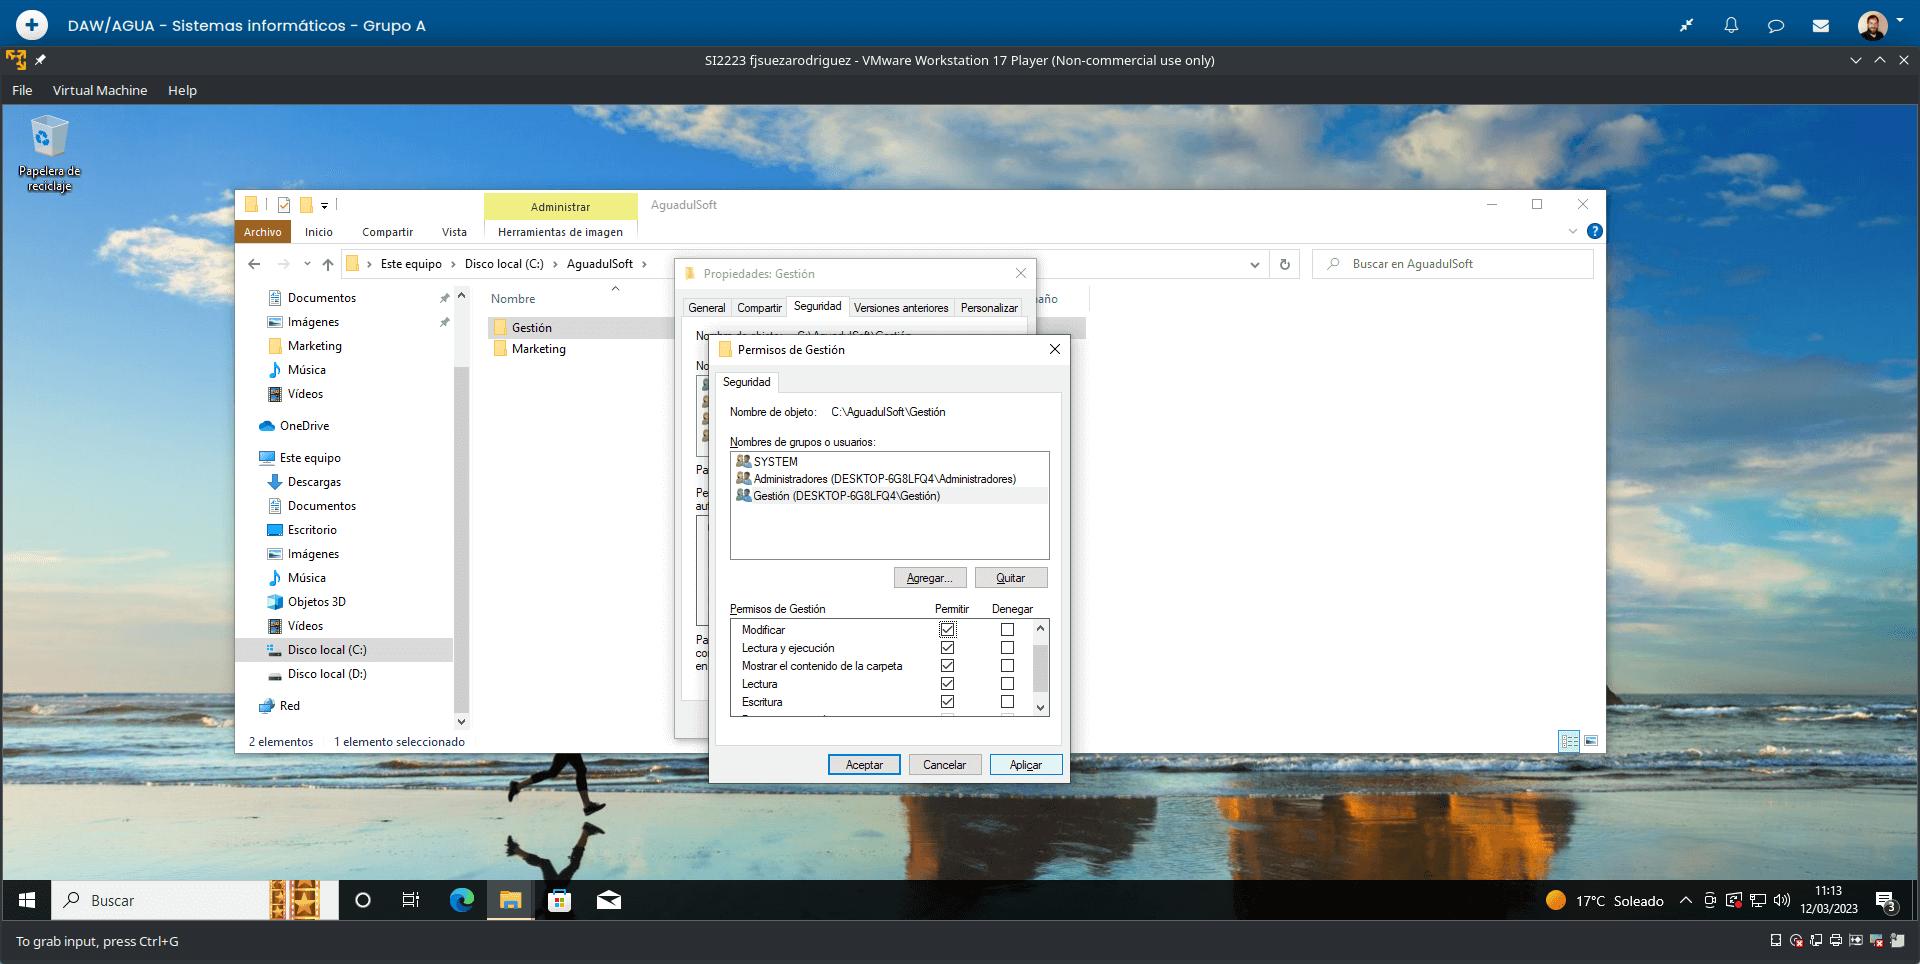
\includegraphics[scale=0.16]{permisos-gestion-nuevos.png}
        \caption{Modificación de los permisos de la carpeta Gestión}
    \end{figure}

    \item A continuación, hemos realizado el mismos procedimiento en la carpeta \textbf{Marketing}, quedando después de la modificación como vemos en la siguiente figura.

    \begin{figure}[H]
        \centering
        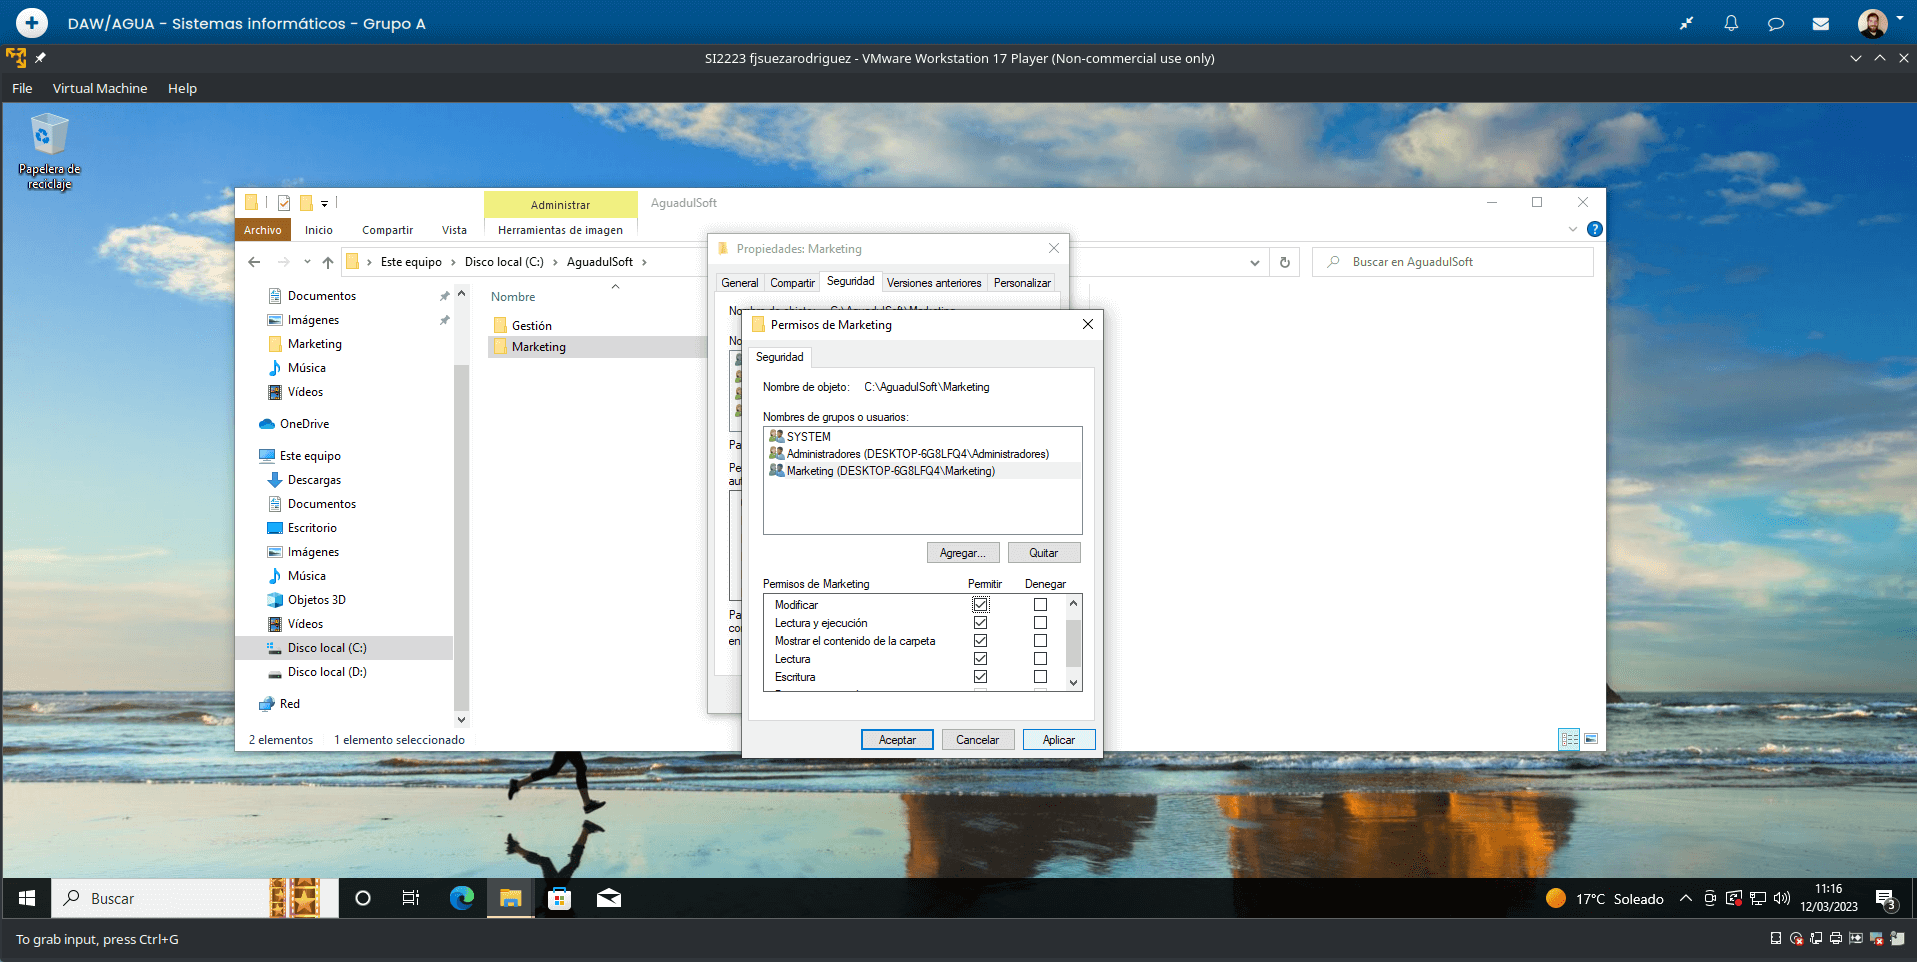
\includegraphics[scale=0.16]{permisos-marketing.png}
        \caption{Modificación de los permisos de la carpeta Marketing}
    \end{figure}

    \item Por último, para \textbf{comprobar que los cambios} se han \textbf{realizado correctamente}, hemos intentado acceder a dichas carpetas con \textbf{usuarios que deberían tener permiso}s y con \textbf{usuarios que no deberían} tenerlos. Hay que tener en cuenta que si el usuario que usamos tiene permisos de administrador se le va a poder habilitar en el directorio concreto, ya que los administrador han conservado sus permisos en dichos directorios.

   Primero hemos intentado acceder a la \textbf{carpeta Gestión} con un \textbf{usuario} perteneciente al \textbf{grupo Gestión}, intentando, posteriormente, acceder con este usuario a la \textbf{carpeta Marketing}. Hemos elegido el usuario \textbf{ggongora}.

   \begin{figure}[H]
       \centering
       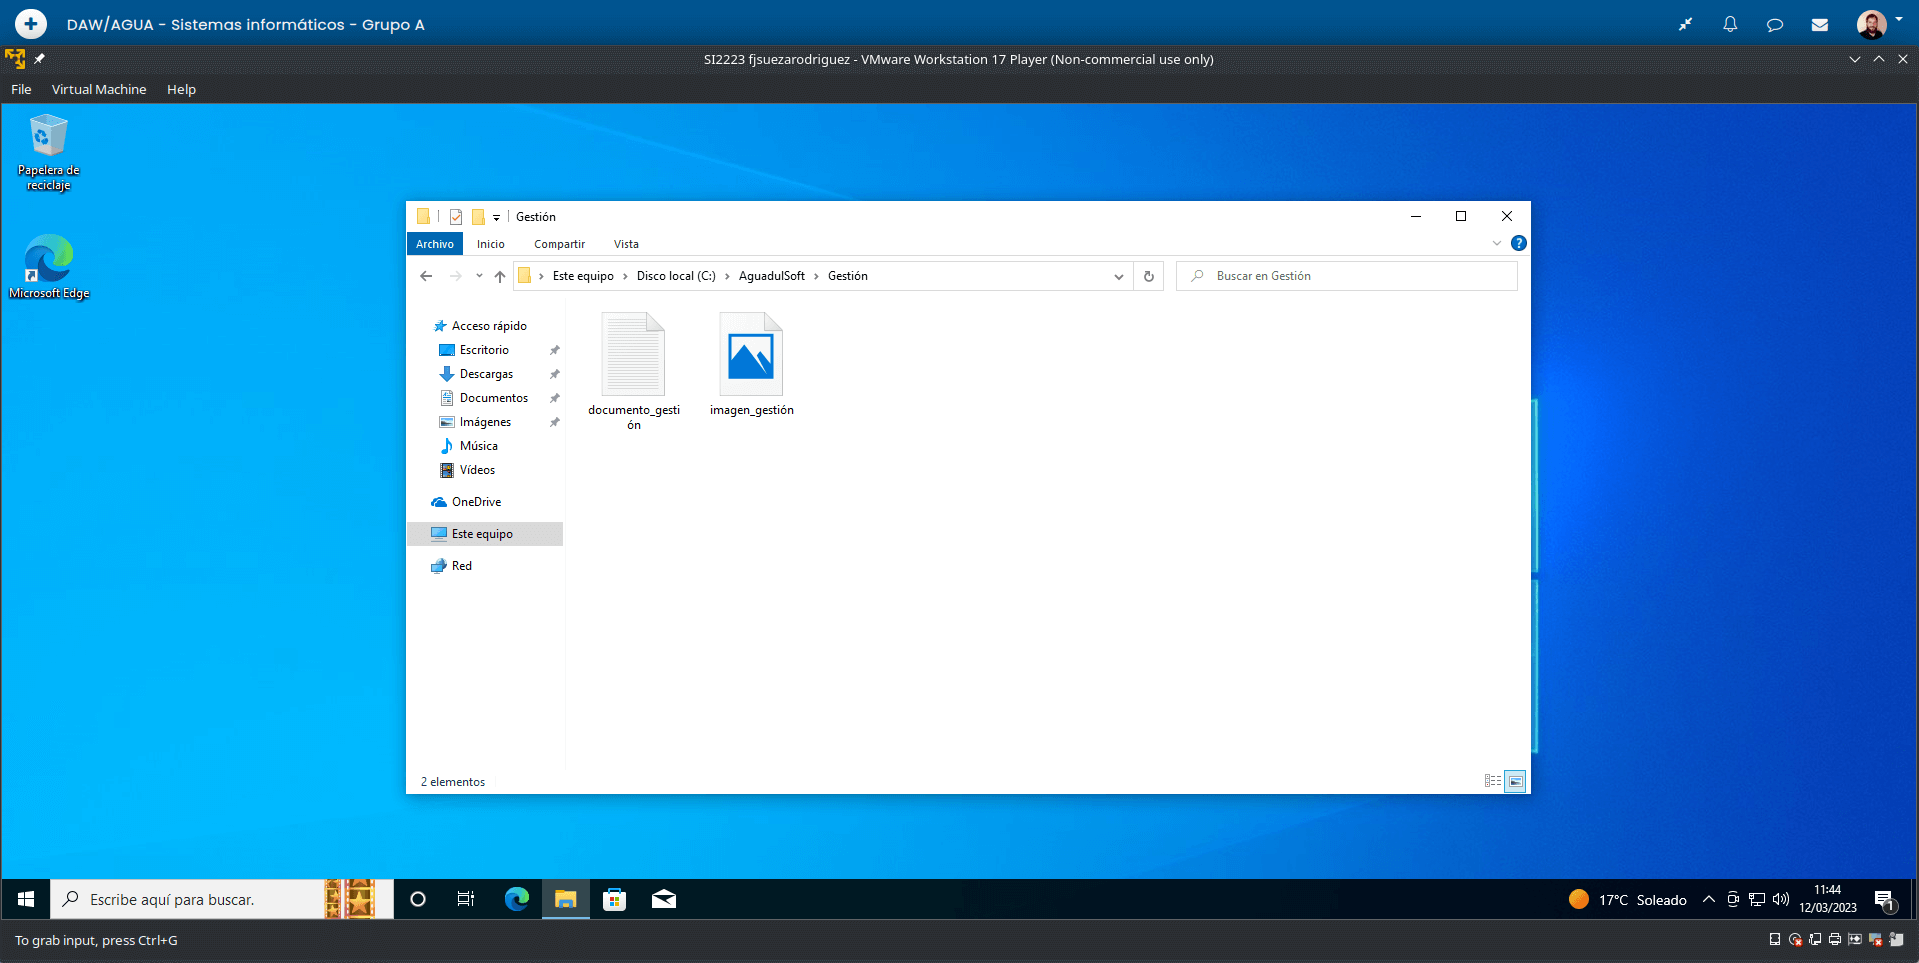
\includegraphics[scale=0.16]{permisos-test-1.png}
       \caption{Acceso a la carpeta Gestión con la usuaria ggongora}
   \end{figure}

    En este caso, \textbf{no hemos tenido ningún problema} de acceder a la carpeta Gestión. Ahora vamos a intentar acceder a la carpeta \textbf{Marketing}.

    \begin{figure}[H]
        \centering
        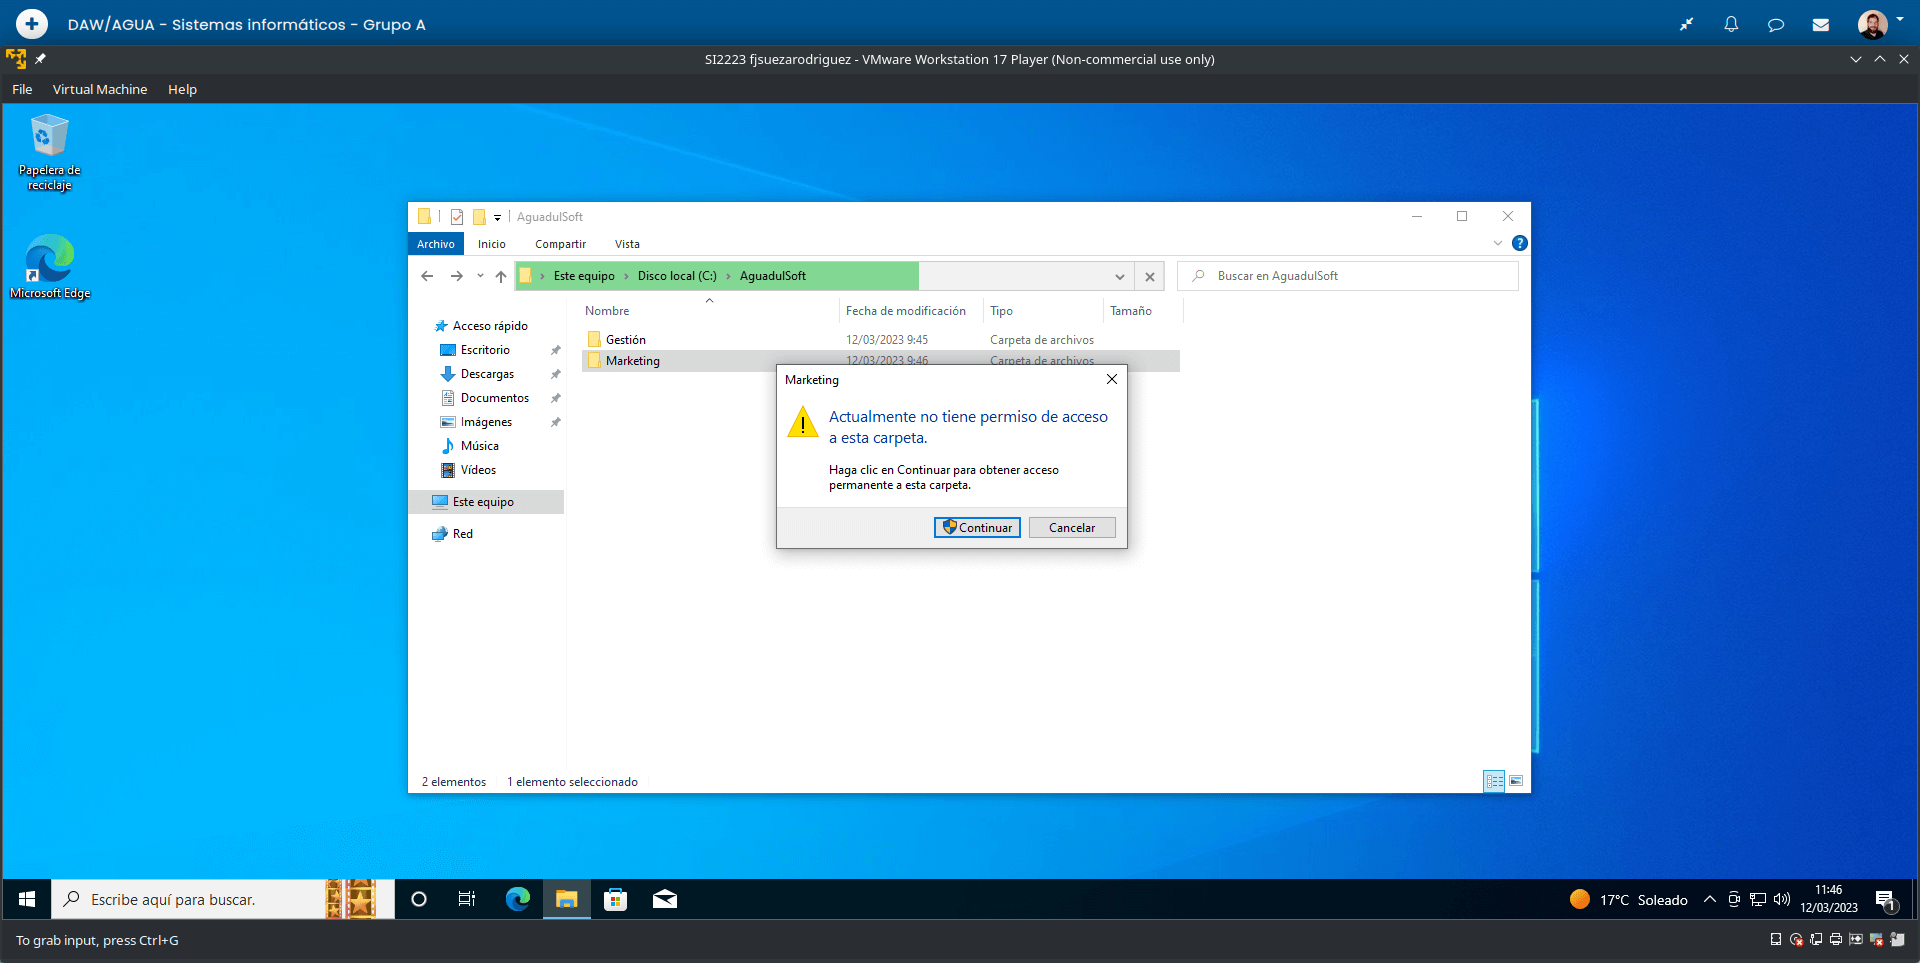
\includegraphics[scale=0.16]{permisos-test-2.png}
        \caption{Acceso a la carpeta Marketing con la usuaria ggongora}
    \end{figure}

    Como vemos, se nos muestra una ventana informándonos de que no tenemos permisos. Como los administradores si los tienen, nos da la opción de agregarnos para tener permisos en esa carpeta, pero como \textit{no sabemos la contraseña de administrador}, no podemos hacerlo. Por último, probamos a entrar en las carpetas con el \textbf{usuario creado} durante \textbf{la instalación} de Windows 10.

   \begin{figure}[H]
        \centering
        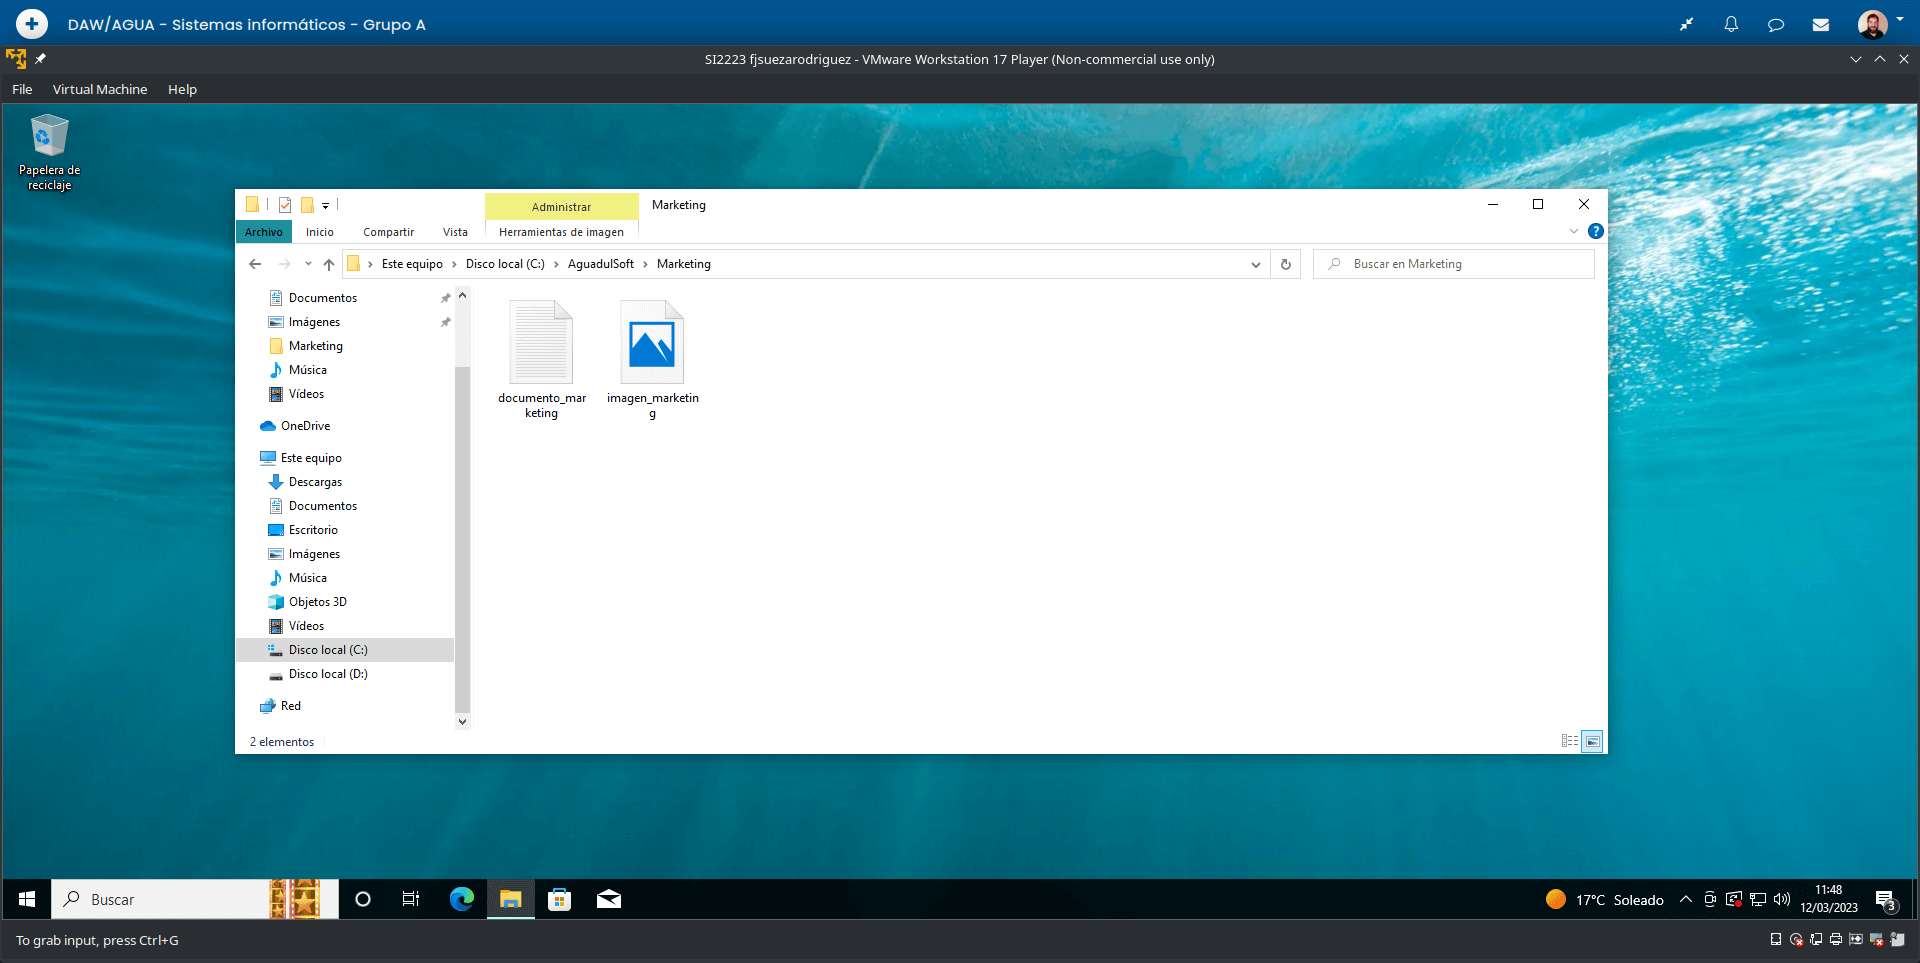
\includegraphics[scale=0.16]{permisos-test-3.png}
        \caption{Acceso a las carpetas con el usuario creado en la instalación}
    \end{figure}

    Como este usuario \textbf{sí tiene permisos de administrador}, no tenemos problemas en acceder a ninguna de las carpetas.
\end{enumerate}

\subsection{Actividad 4: Directivas de Seguridad y Grupo Local}

\subsubsection{Enunciado}
\begin{enumerate}[label=\alph*)]
    \item Habilita las \textbf{directivas seguridad} de contraseñas correspondientes para que el sistema guarde el registro de las \textbf{5 últimas contraseñas} de usuario, requiera que sean \textbf{complejas}, tengan una vigencia máxima de \textbf{30 días} y una longitud mínima de \textbf{10 caracteres}. Establece también que se permitan hasta 3 equivocaciones de un usuario al iniciar sesión, y que en el caso de producirse la cuenta del usuario quede bloqueada durante \textbf{15 minutos}.

    \textbf{Capturas}:
    \begin{itemize}
        \item Ventana donde se asignan las directivas de contraseñas y de bloqueo de cuenta (indica textualmente cómo se accede a dicha ventana).
        \item Proceso de asignación de las directivas de contraseñas exigidas.
        \item Resumen de asignación de las directivas de contraseñas aplicadas.
        \item Proceso de asignación de las directivas de bloqueo de cuenta exigidas.
        \item Resumen de asignación de las directivas de bloqueo de cuenta aplicadas.
    \end{itemize}

    \item \textbf{Directiva de grupo local}: Impide el acceso de los usuarios al símbolo del sistema editando las directiva correspondiente.

    A continuación, para comprobar que se ha realizado correctamente, muestra qué ocurre cuando intentas acceder al símbolo del sistema.

    \textbf{Capturas}:
        \begin{itemize}
            \item Ventana donde se asignan las directivas de grupo local (indica textualmente cómo se accede a dicha ventana).
            \item Proceso para impedir el acceso de los usuarios al símbolo del sistema.
            \item Intento de acceso al símbolo del sistema.
        \end{itemize}
\end{enumerate}

\subsubsection{Solución}

En este ejercicio vamos a configurar y modificar las directivas de seguridad en Windows 10, tanto las locales como las de grupos.

\begin{enumerate}
    \item En primer lugar vamos a modificar las directivas de seguridad, en concreto, las \textbf{directivas de cuenta}, para añadir ciertas \textbf{restricciones} tanto a la \textbf{creación de contraseñas} como establecer ciertos parámetros para el \textbf{bloqueo de cuentas}.

    Para acceder a al aplicación de \textbf{Directivas de seguridad local}, solo debemos buscar la aplicación por su nombre en la \textbf{búsqueda} de la barra de Windows 10, a la derecha del \textbf{Menu Inicio}. El primer resultado que nos arroja es dicha aplicación. Ya solo debemos pulsar en \textbf{Ejecutar como administrador} para iniciarla.

    Una vez con la aplicación abierta, seleccionamos la carpeta \textbf{Directivas de Cuenta} y se nos mostrarán 2 subcarpetas, \textbf{Directiva de contraseña} y \textbf{Directiva de bloque de cuenta}, en las cuales podremos realizar los cambios que nos pide el enunciado.

    \begin{figure}[H]
        \centering
        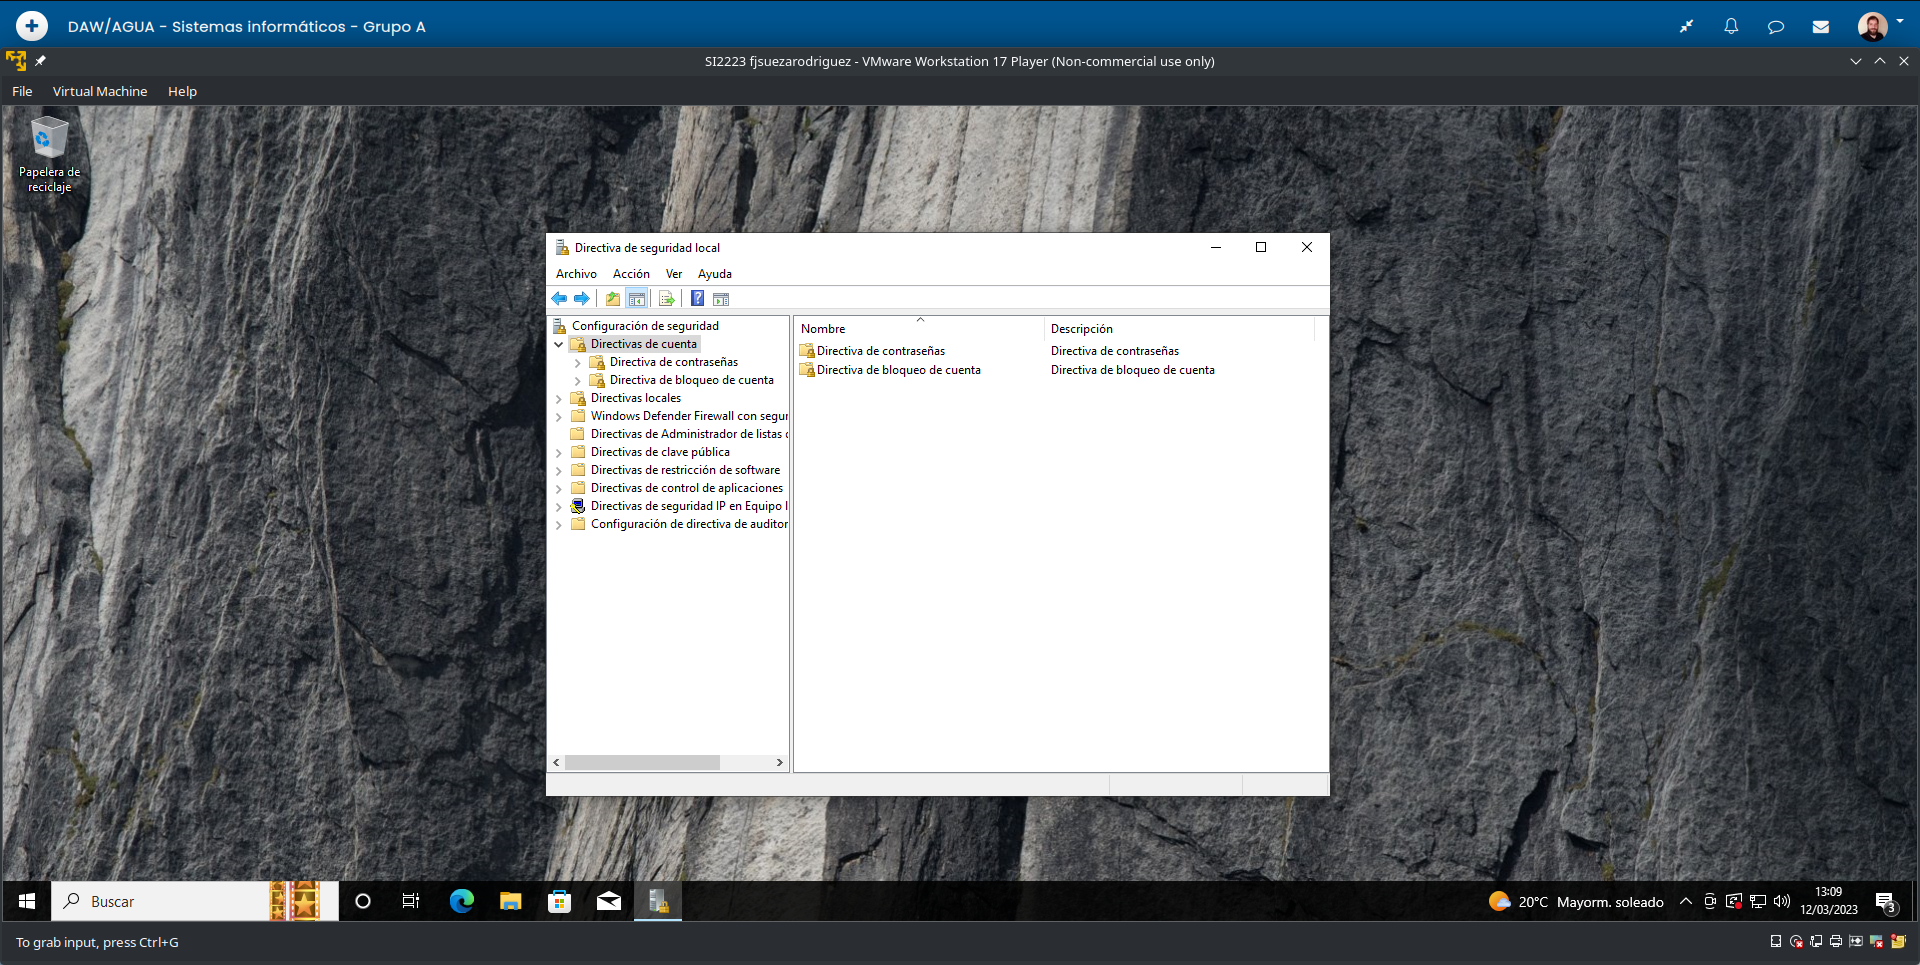
\includegraphics[scale=0.16]{directivas-ventana.png}
        \caption{Ventana para el cambio de directivas de cuenta}
    \end{figure}

    Para cambiar las directivas respecto a las contraseñas, debemos pulsar en la opción \textbf{Directivas de contraseña}. Estos nos desplegará un conjunto de opciones que podremos ir cambiando.

    \begin{figure}[H]
        \centering
        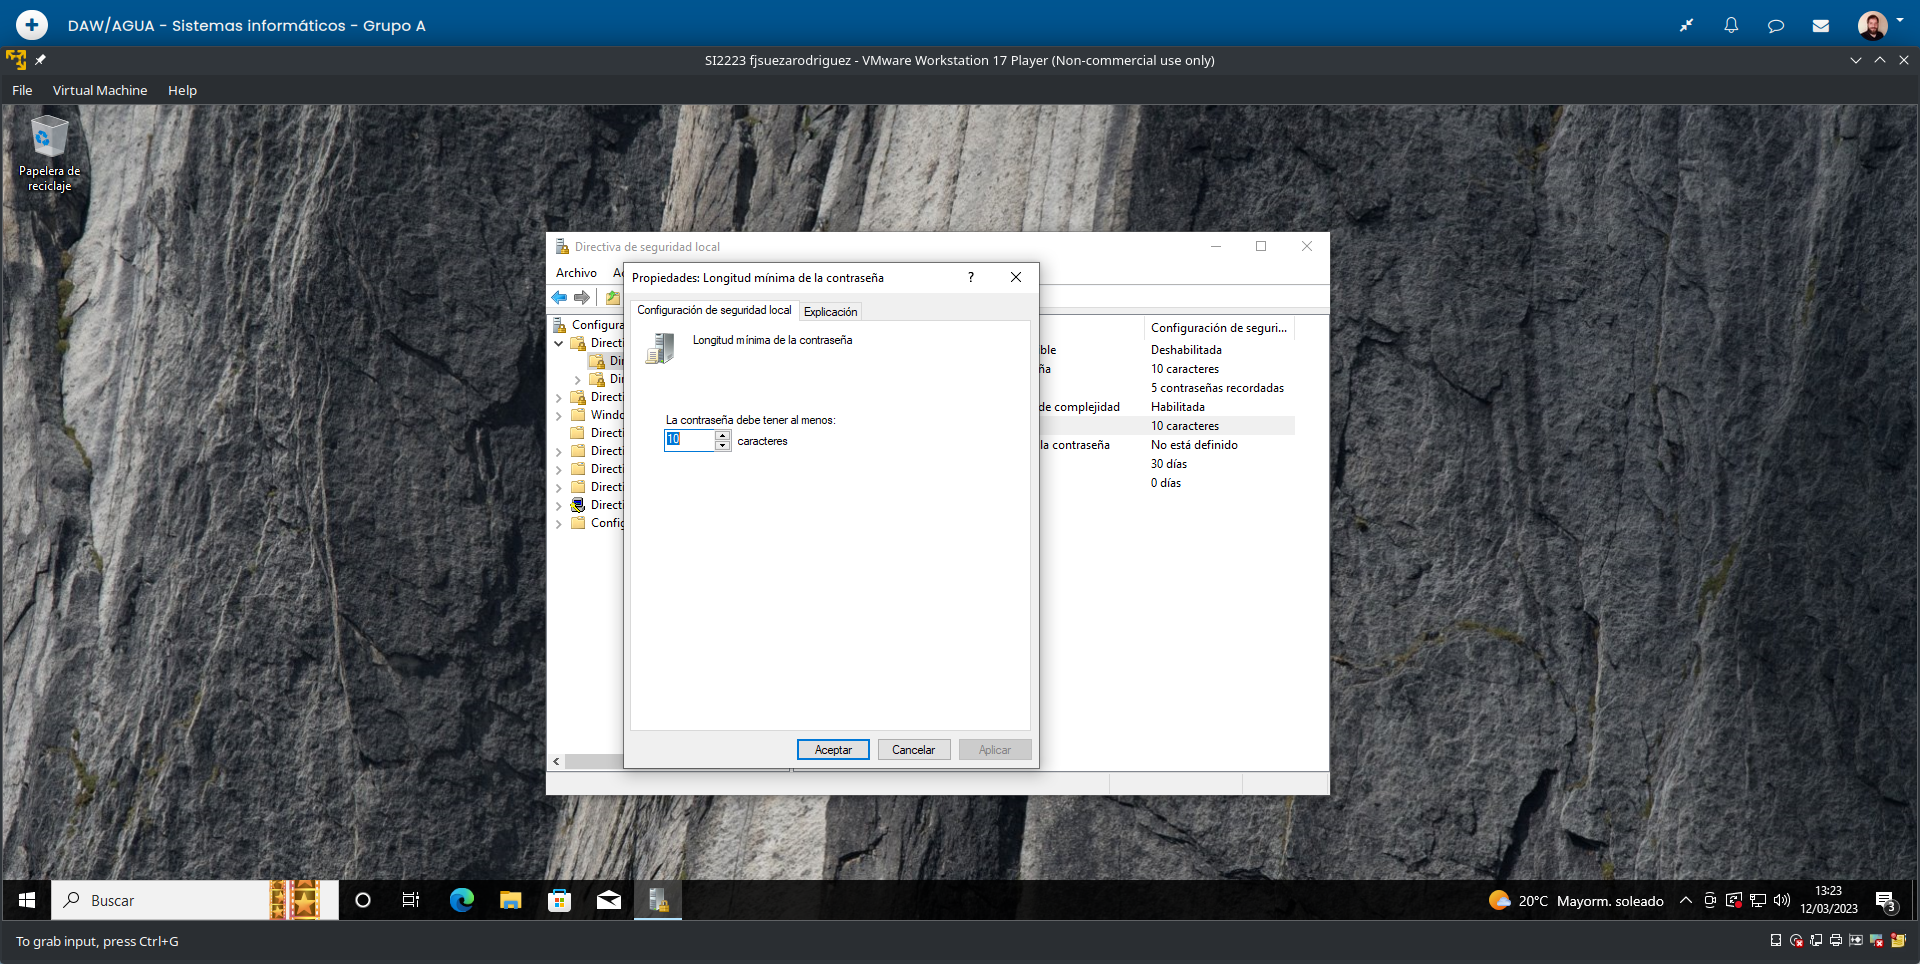
\includegraphics[scale=0.16]{directivas-pass-1.png}
        \caption{Cambio de la longitud de contraseña requerida}
    \end{figure}

    Tras realizar todas las modificaciones solicitadas, las directivas de contraseña quedan de la siguiente manera.

    \begin{figure}[H]
        \centering
        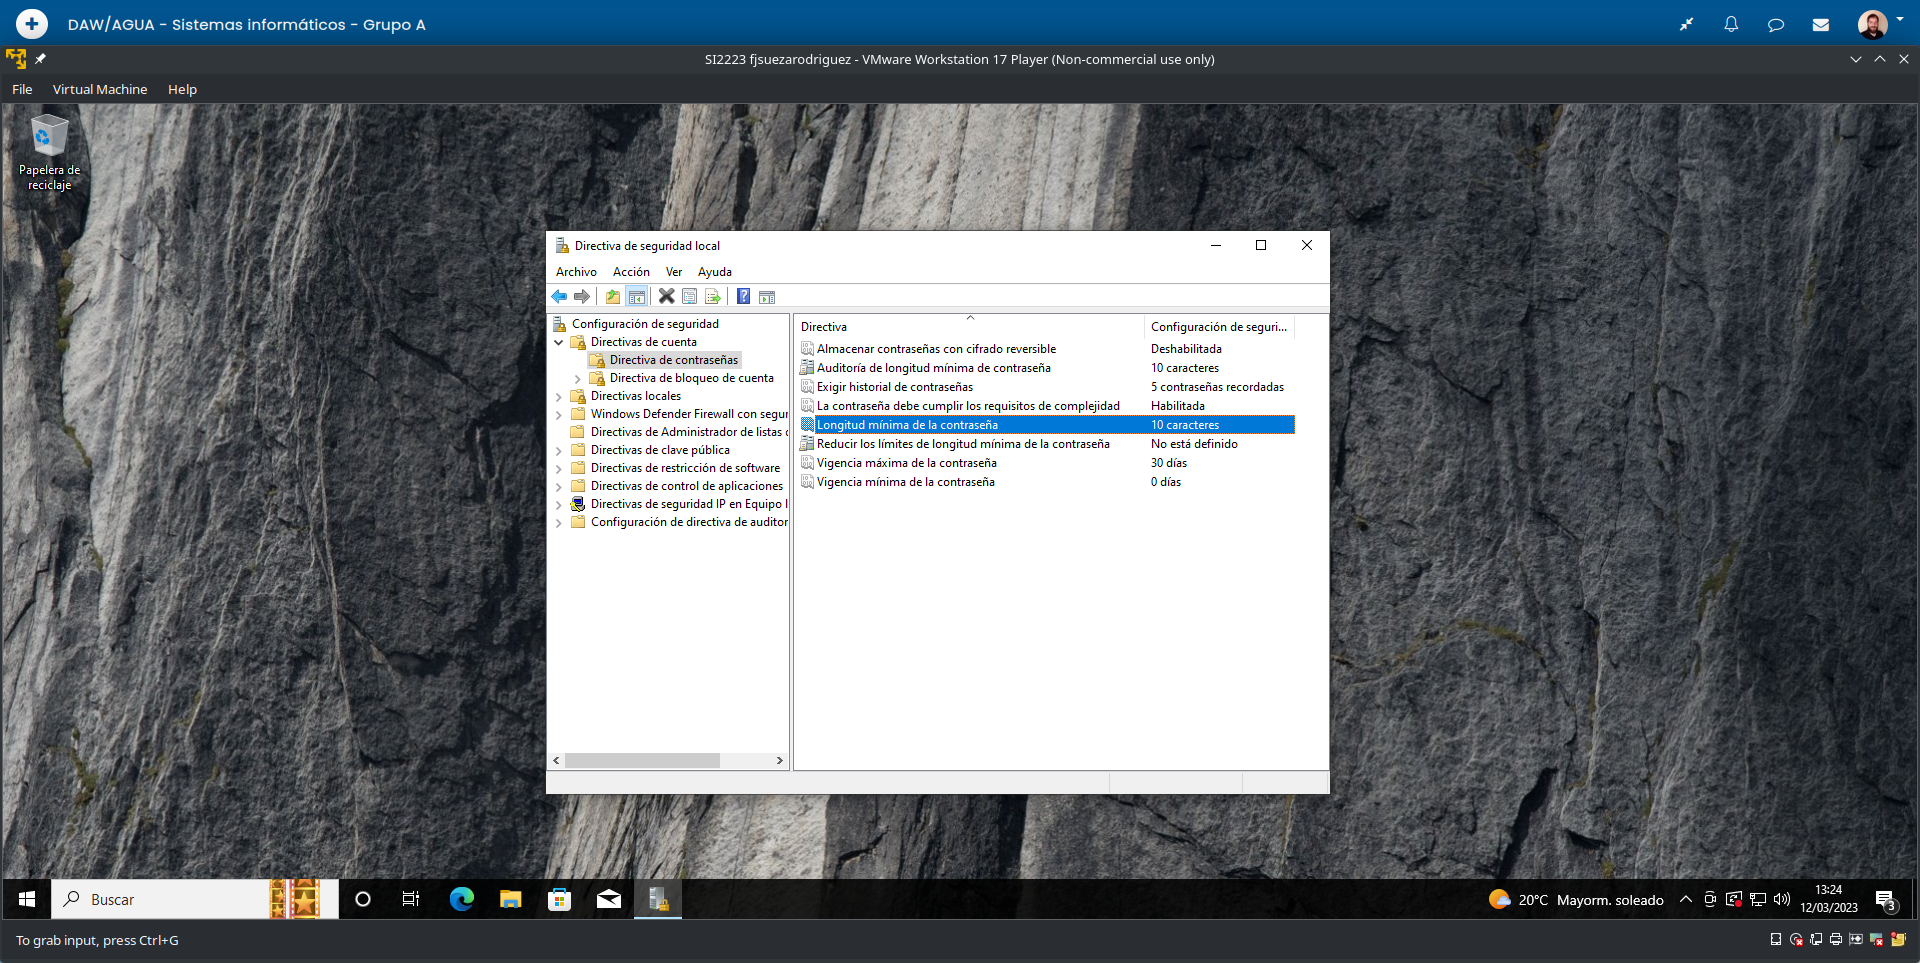
\includegraphics[scale=0.16]{directivas-pass-2.png}
        \caption{Resumen de las directivas de contraseña}
    \end{figure}

    A continuación, desde la carpeta de \textbf{Directivas de cuenta}, pulsamos sobre la opción \textbf{Directiva de bloqueo de cuenta}. Al igual que en la acción anterior, se nos mostrará un conjunto de opciones que podremos modificar, con una diferencia, y es que para que las opciones \textbf{Duración del bloque de cuenta} y \textbf{Restablecer bloque de cuentas despues de} se nos habiliten, primero debemos establecer un número de intentos predeterminados con la opción \textbf{Umbral de bloque de cuenta}, como vemos en la siguiente figura.

    \begin{figure}[H]
        \centering
        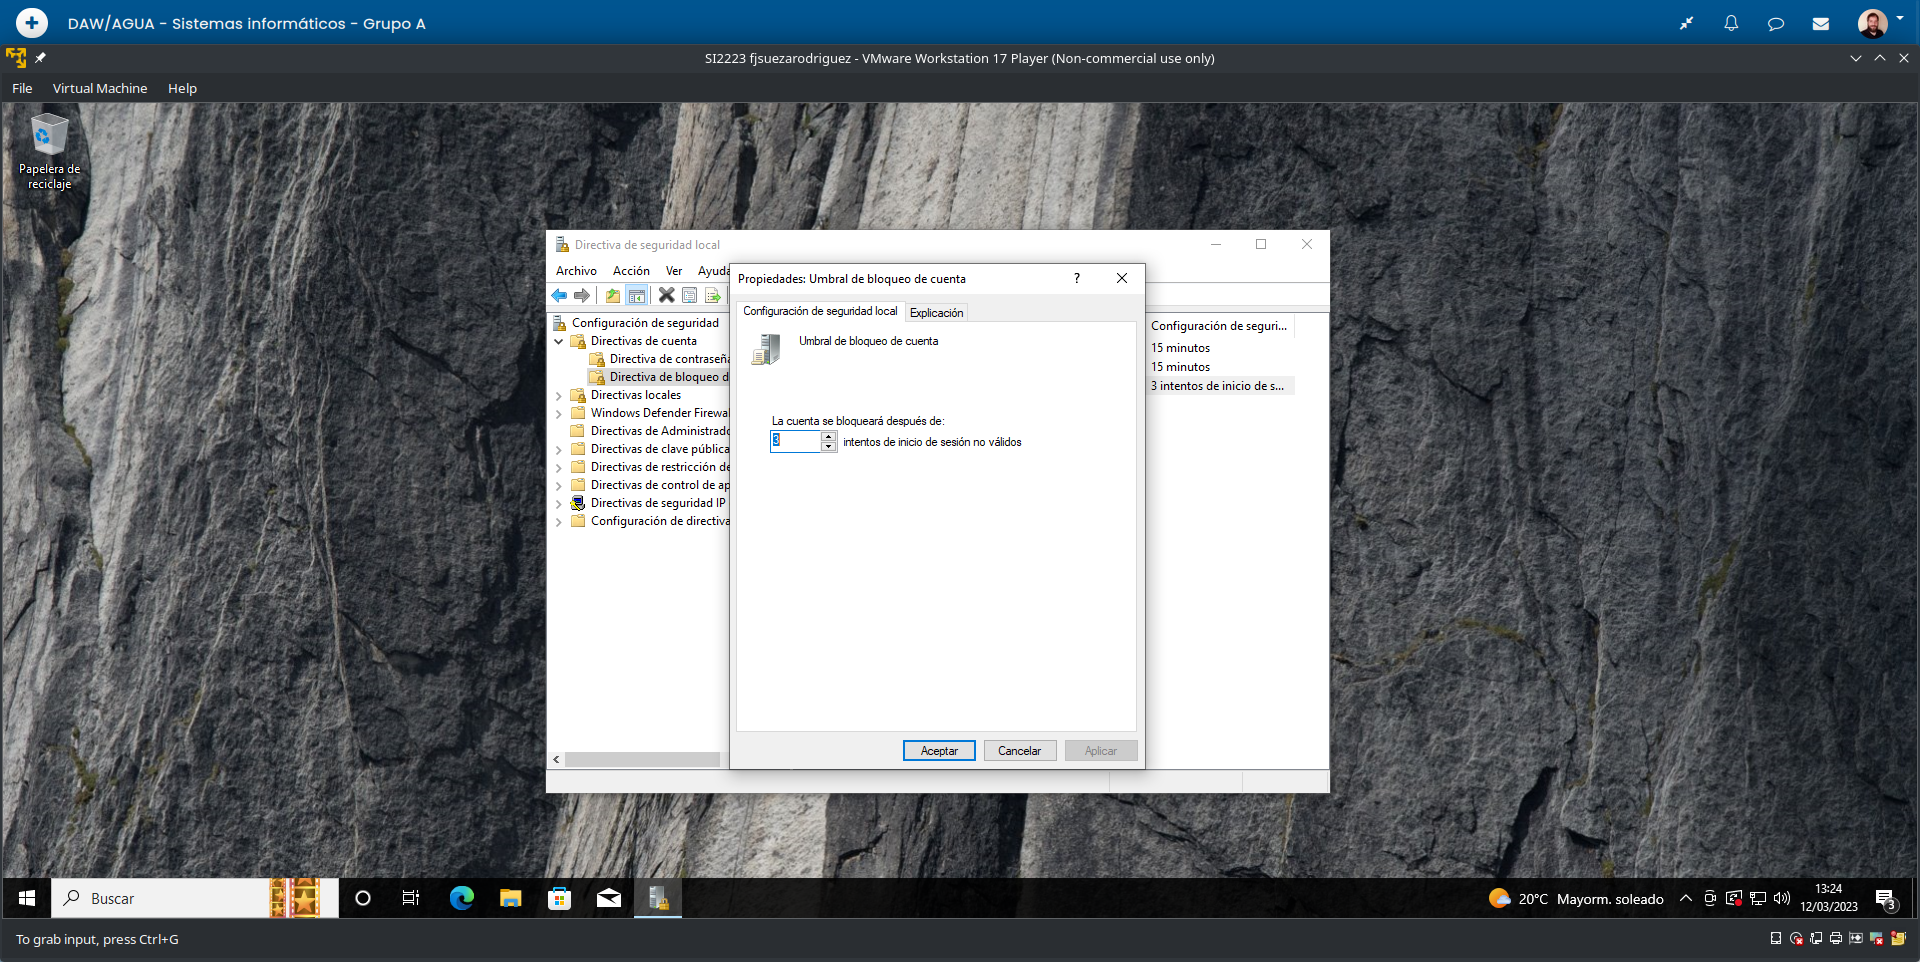
\includegraphics[scale=0.16]{directivas-bloq-1.png}
        \caption{Cambio del umbral de bloque de cuenta}
    \end{figure}

    Una vez realizado esto, ya podremos cambiar las otras dos opciones, quedando las directivas de bloque de cuenta como podemos ver a continuación.

    \begin{figure}[H]
        \centering
        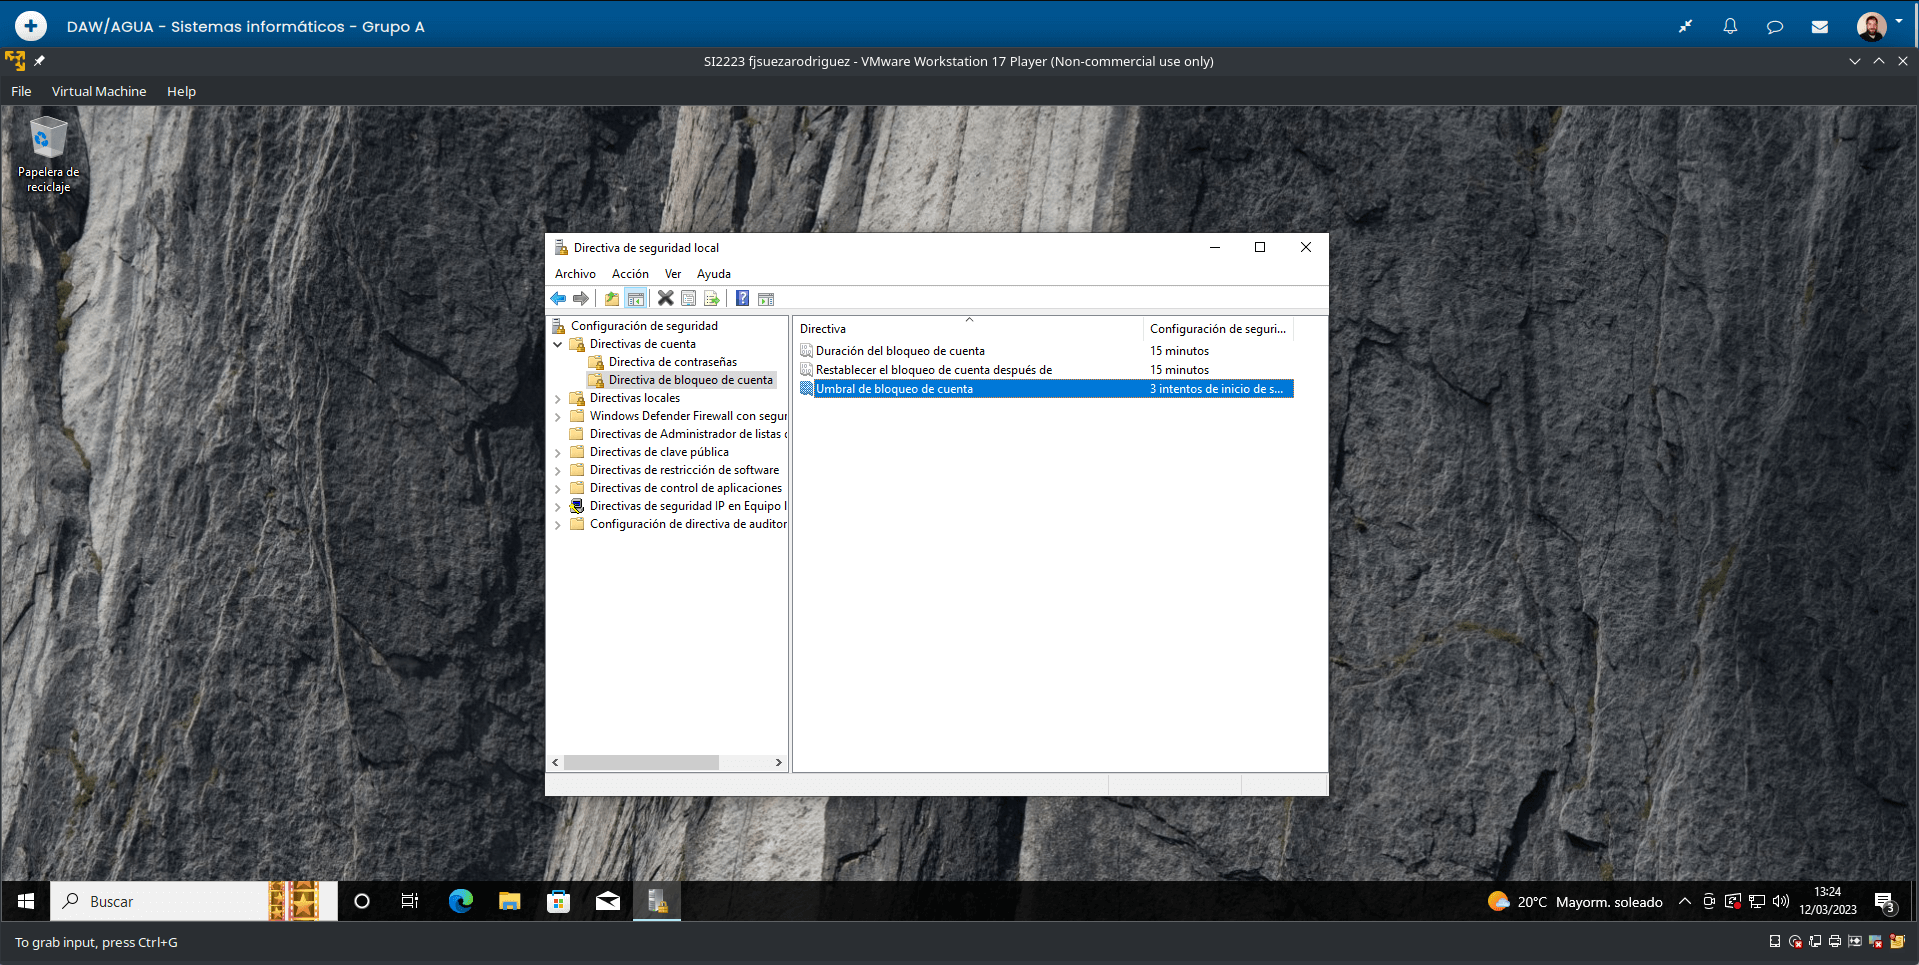
\includegraphics[scale=0.16]{directivas-bloq-2.png}
        \caption{Resumen de la directivas de bloque de cuenta}
    \end{figure}

    \item Una vez cambiadas las directivas de cuentas, vamos a proceder a modificar las \textbf{Directivas de grupo local}, impidiendo el acceso al \textbf{símbolo del sistema} a los usuarios.

    Para ello, hemos usado el comando \textbf{gpedit.msc}, introducido desde la consola. Eso nos abrirá la aplicación, que nos mostrará multitud de opciones para modificar las directivas locales, resaltando dos opciones principales: \textbf{Configuración de Equipo} y \textbf{Configuración de Usuario}. Esta última es la que nos interesa a nosotros, como veremos en el siguiente paso.

    \begin{figure}[H]
        \centering
        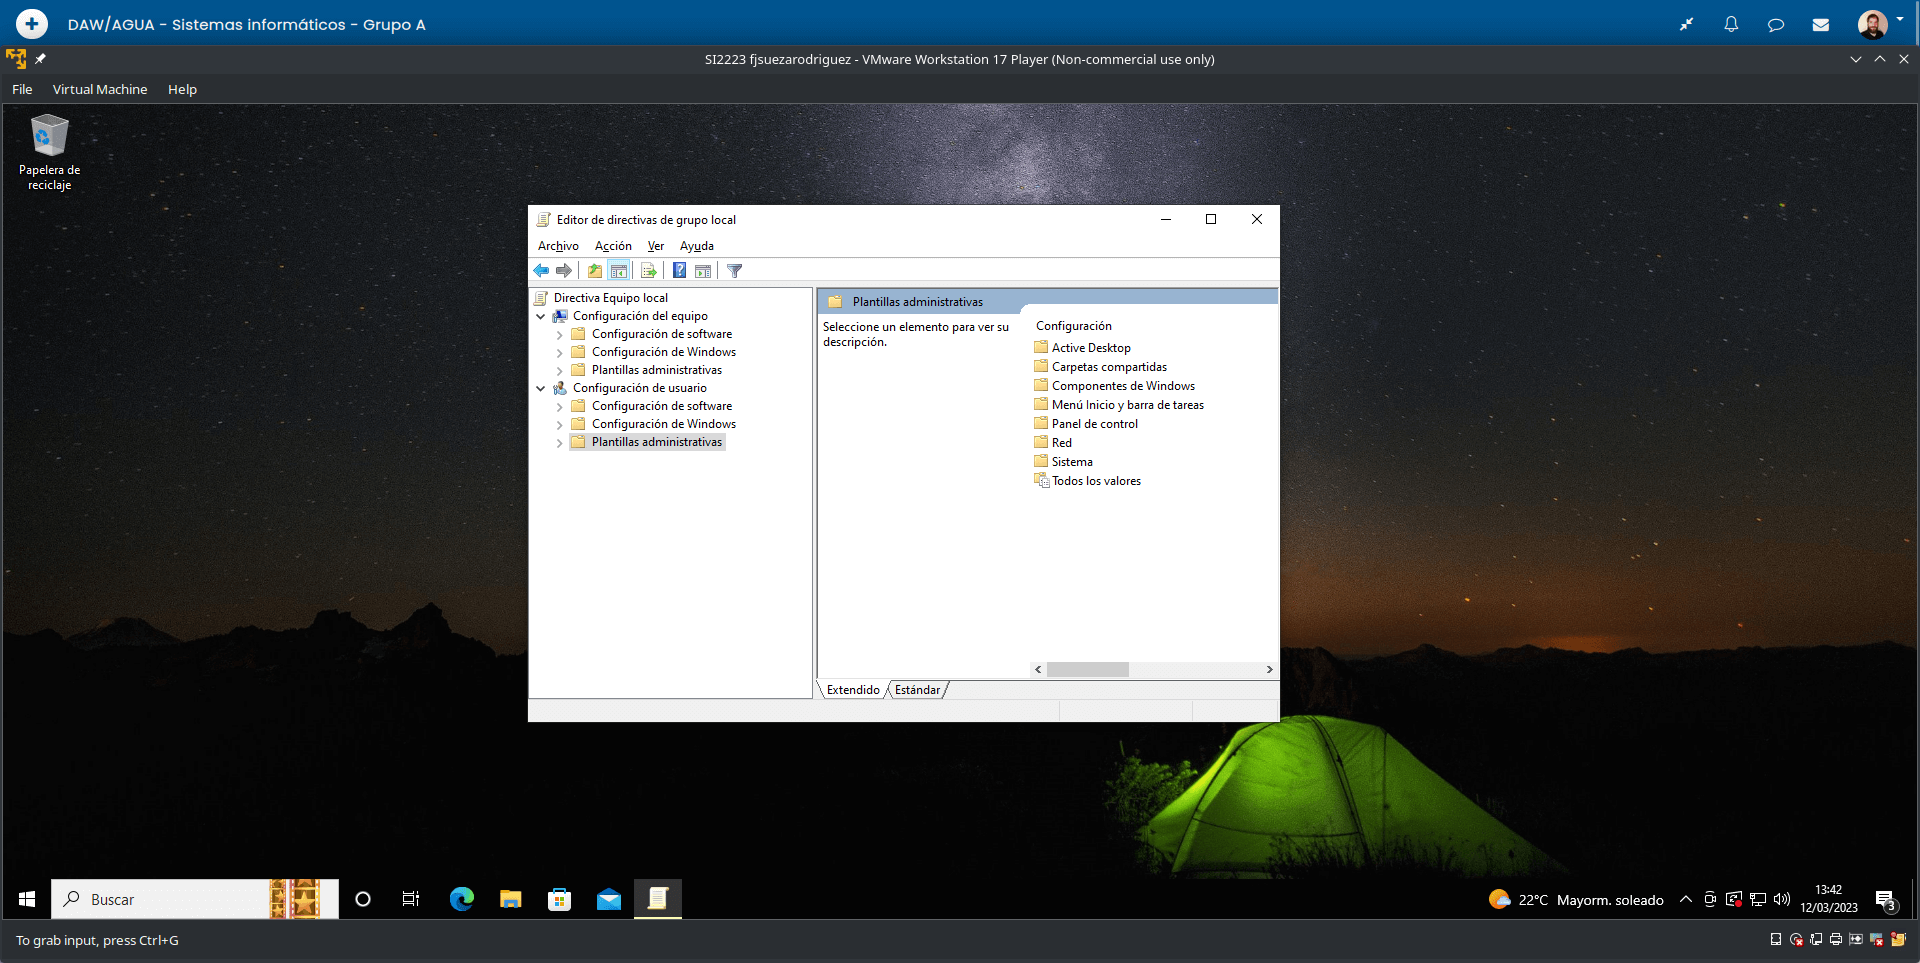
\includegraphics[scale=0.16]{directiva-local-1.png}
        \caption{Ventana de la aplicación gpedit para modificar la directivas de grupo local}
    \end{figure}

    Una vez abierta la aplicación, debemos buscar la opción para \textbf{impedir el acceso de los usuarios al símbolo de sistema}. Para llegar a esta opción debemos pulsar en \textbf{Configuración de Usuario ---> Plantillas Administrativas ---> Sistema}.  Aquí, si nos fijamos en la parte derecha de la ventana, nos saldrán un conjunto de carpetas y directivas que configurar, entre las que podemos encontrar \textbf{Impedir el acceso al símbolo del sistema}. Debemos pulsar en esta opción, lo que nos abrirá una ventana con una explicación sobre el funcionamiento de esta directiva y como cambiarla.

    \begin{figure}[H]
        \centering
        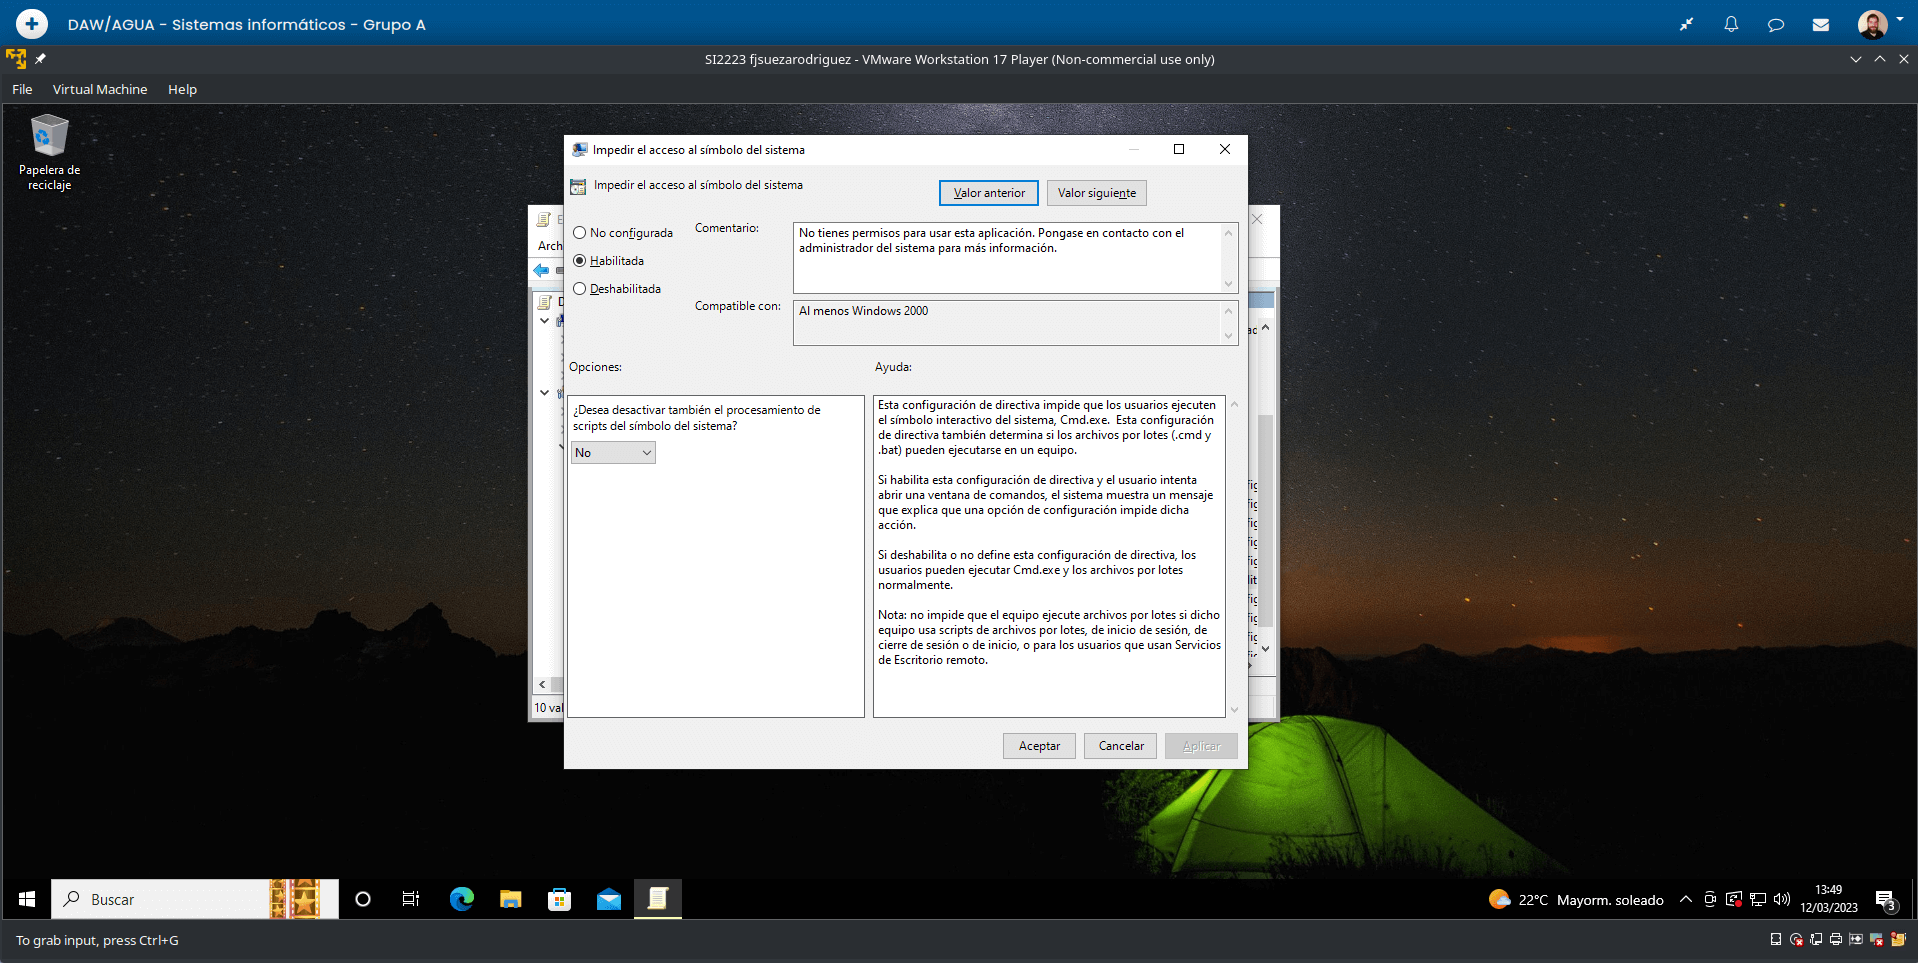
\includegraphics[scale=0.16]{directiva-local-2.png}
        \caption{Directiva para impedir el acceso al símbolo del sistema}
    \end{figure}

    Una vez cambiada, no se podrá acceder al símbolo del sistema, ni siquiera, teniendo permisos de administrador, como vemos en la siguiente captura.

    \begin{figure}[H]
        \centering
        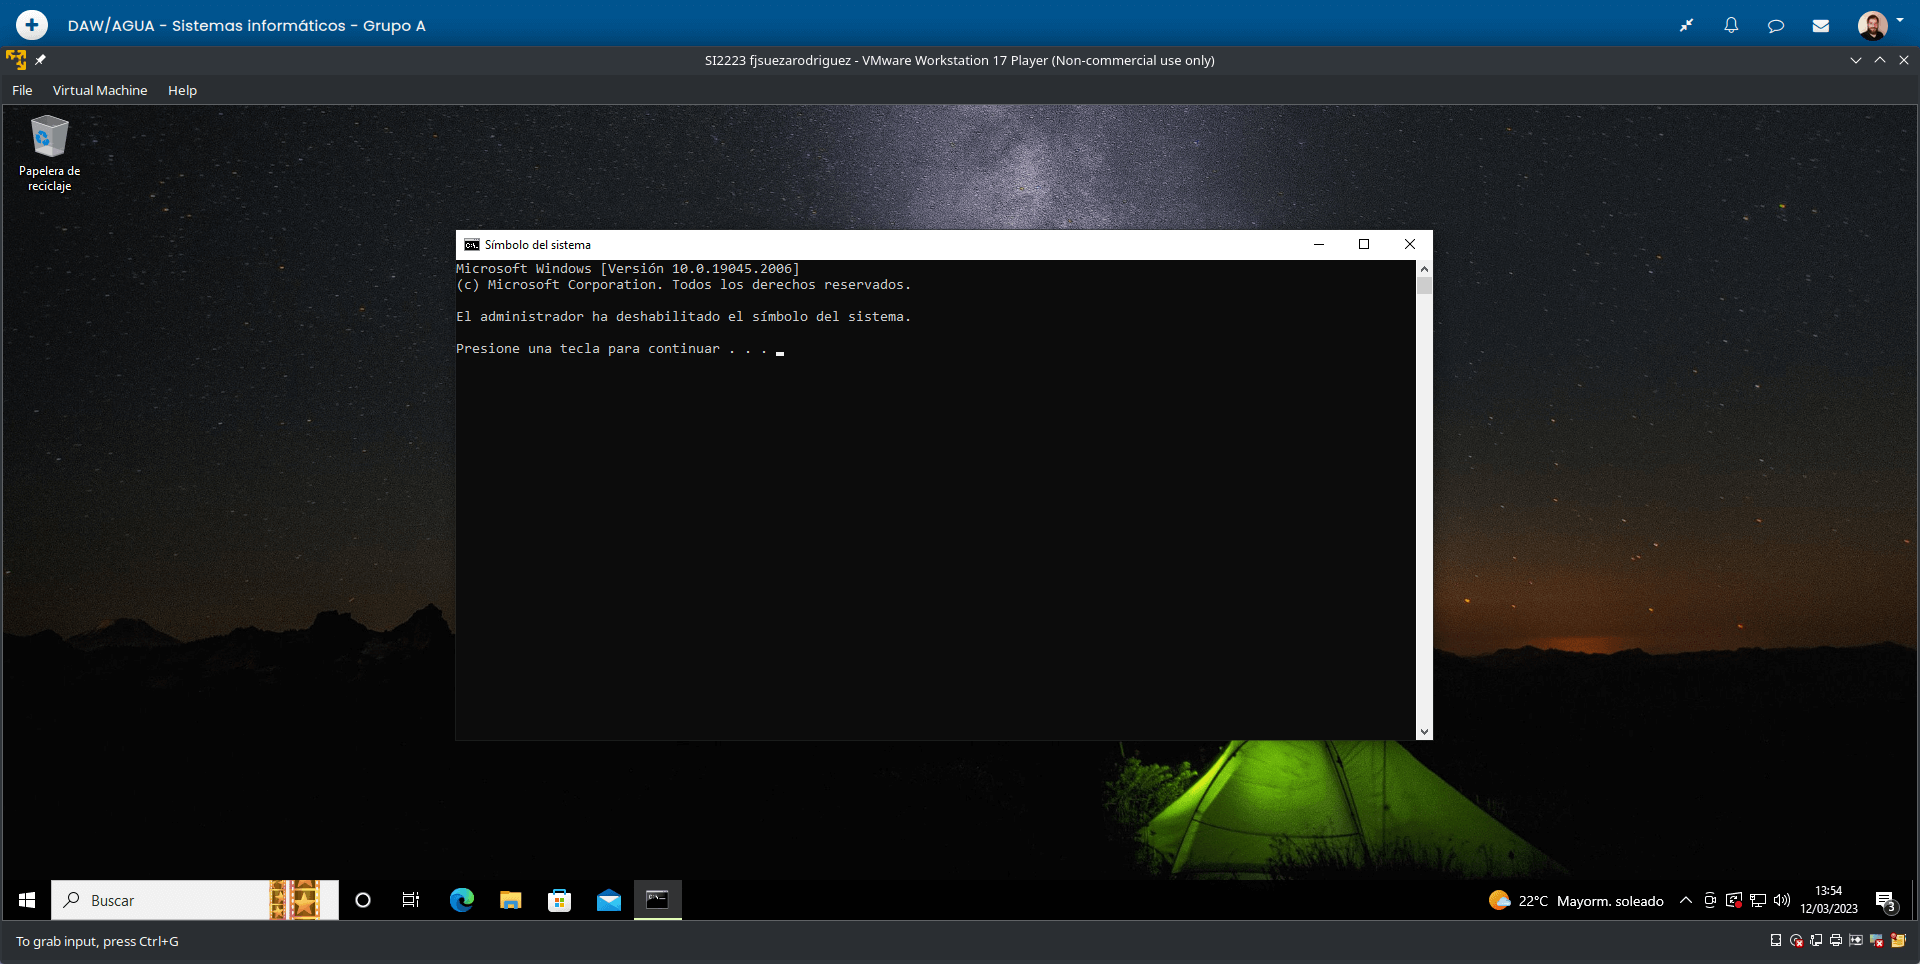
\includegraphics[scale=0.16]{directiva-local-3.png}
        \caption{Intento de acceso al símbolo del sistema}
    \end{figure}
\end{enumerate}

\subsection{Windows Defender: Programar Análisis}
\subsubsection{Enunciado}
Si tienes instalado un software antivirus en tu MV, activa la ejecución periódica de Windows Defender.

Si no tienes ningún antivirus de terceros instalado, accede a ``Protección Antivirus y contra amenazas'' y asegúrate de que tienes todas las protecciones habilitadas (en tiempo real, en la nube, envío de muestras automático, contra alteraciones, ...). Esta protección no ralentiza mucho el sistema y puede ser suficiente para evitar software indeseado, aunque debes mantener siempre actualizado el sistema con las updates de seguridad.

Accede a la Biblioteca del Programador de Tareas, y en la carpeta Microsoft\textbackslash Windows\textbackslash Windows Defender, modifica la tarea que realiza el análisis ``Windows Defender Scheduled Scan'' para que no se ejecute en una hora programada, sino cuando se registre un evento de categoría ``Registros de Windows'' (subcategorías ``Aplicación'', ``Seguridad'', ``Instalación'', ``Sistema'' y ``Eventos reenviados''), de nivel crítico o de error, y además haya ocurrido en la última hora. Para todo esto debes crear un filtro de eventos personalizado.

\textbf{Capturas}:

\begin{itemize}
    \item Ventana de configuración donde se verifica que todas las protecciones están activas, o que se permite examen periódico de Windows Defender (en caso de tener un antivirus externo).
    \item Abre la tarea modificada y muestra la pestaña ``Desencadenadores'' con el máximo nivel de detalle (indica textualmente cómo realizas el acceso).
    \item Muestra el filtro personalizado en formato XML.
\end{itemize}

\subsubsection{Solución}
En este ejercicio vamos a realizar la configuración de \textbf{Windows Defender} para que realice exámenes de forma periódica, así como a comprobar que todas las protecciones están habilitadas.

\begin{enumerate}
    \item En primer lugar, hemos comprobado que tenemos todas las protecciones activadas. Lo cual podemos hacer en \textbf{Protección antivirus y contra amenazas}. Como podemos ver en la siguiente captura, todas las protecciones están activadas correctamente.

    \begin{figure}[H]
        \centering
        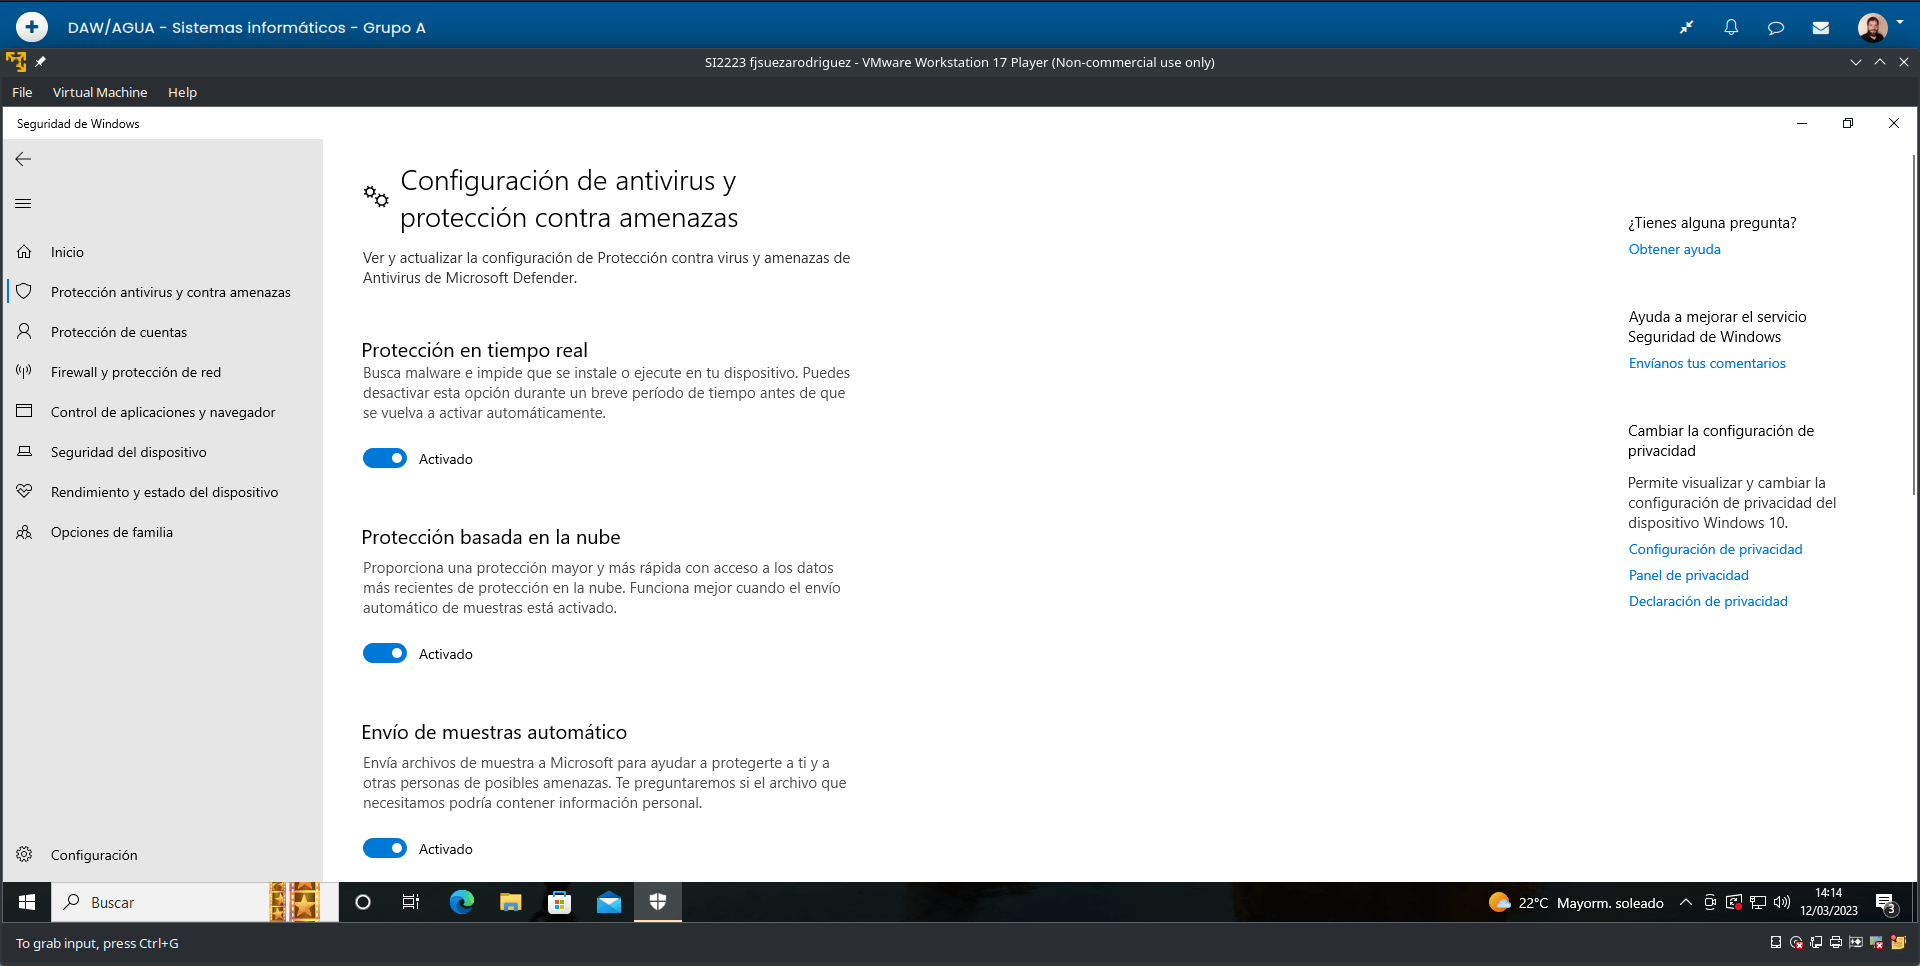
\includegraphics[scale=0.16]{defender-1.png}
        \caption{Protección antivirus y otras amenazas}
    \end{figure}

    \item Una vez hemos comprobado que tenemos todas las protecciones activas, vamos a modificar la tarea de sistema que se encarga de ejecutar Windows Defender.

    Para ello, en primer lugar, abrimos la aplicación \textbf{Programador de tareas}, buscando la barra de búsqueda del sistema. Una vez abierta la aplicación, la opción de Windows defender se encuentra en la ruta de carpetas \textbf{Biblioteca del programador de tareas ---> Windows ---> Windows Defender}.

    Una vez abierta esta carpeta, se nos mostrarán las diferentes tareas vinculadas a Windows Defender, aunque a nosotros la que nos interesa es \textbf{Windows Defender Schedule Scan}. Pulsamos con el botón derecho sobre esta tarea y seleccionamos la opción \textbf{Propiedades}.

    Se nos abrirá una ventana con las propiedades de la tarea. Nosotros, vamos a pulsar sobre la pestaña \textbf{Desencadenadores} y a añadir uno nuevo, pulsando en el botón \textbf{Nuevo}. En la ventana que se nos abre, deberemos seleccionar la opción \textbf{Al producirse un evento} en el menú desplegable \textbf{Iniciar tarea}, y posteriormente marcar la opción \textbf{Personalizada} en el recuadro inferior, lo que nos mostrará el botón de \textbf{Nuevo filtro de evento...}, el cual vamos a pulsar.

    En esta nueva ventana, en primer lugar vamos a seleccionar la opción \textbf{Última hora} en el menú desplegable \textbf{Registrado}. A continuación marcamos \textbf{Crítico} y \textbf{Error} en las opciones de \textbf{Nivel de evento}. Por último seleccionamos la opción \textbf{Registros de Windows}, en el menú desplegable \textbf{Registro de eventos}. Eso no seleccionará automáticamente todos los eventos de los registros de Windows.

    \begin{figure}[H]
        \centering
        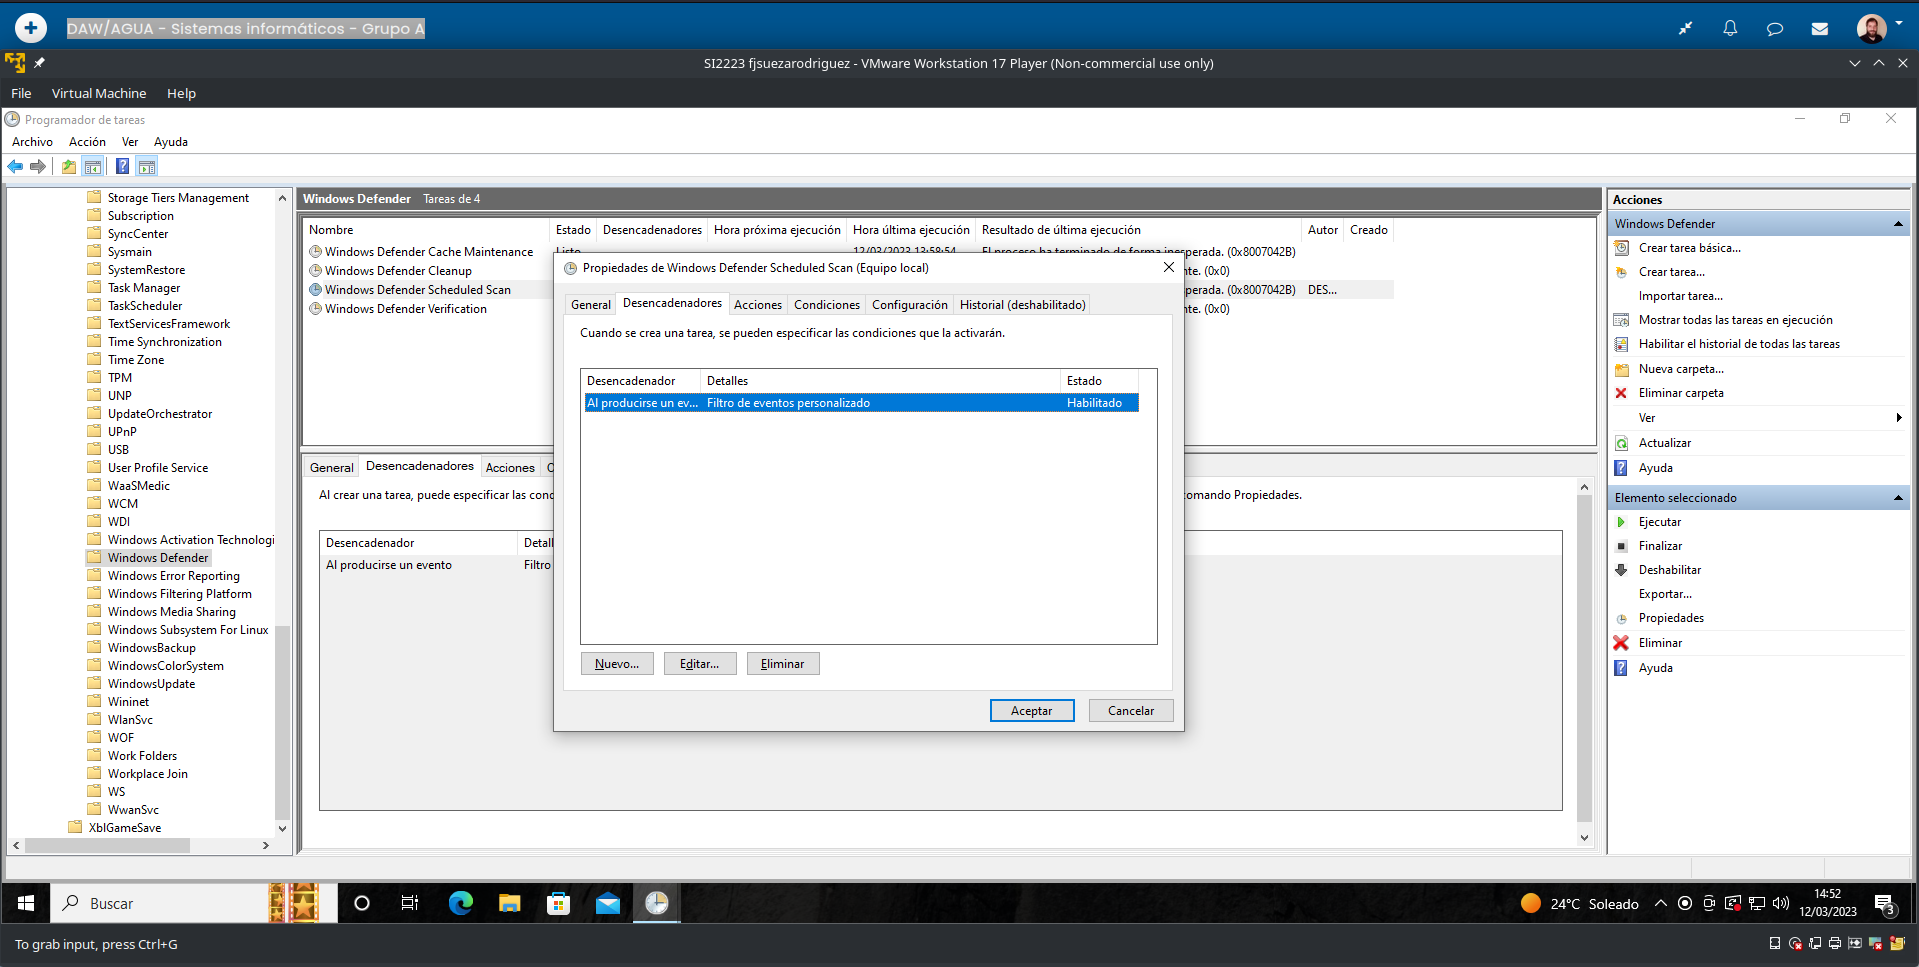
\includegraphics[scale=0.18]{defender-2.png}
        \caption{Desencadenador creado para la tarea de Windows Defender}
    \end{figure}

    Una vez modificada la tarea y creado el nuevo filtro, mostramos la salida en XML del nuevo filtro de evento creado.

    \begin{figure}[H]
        \centering
        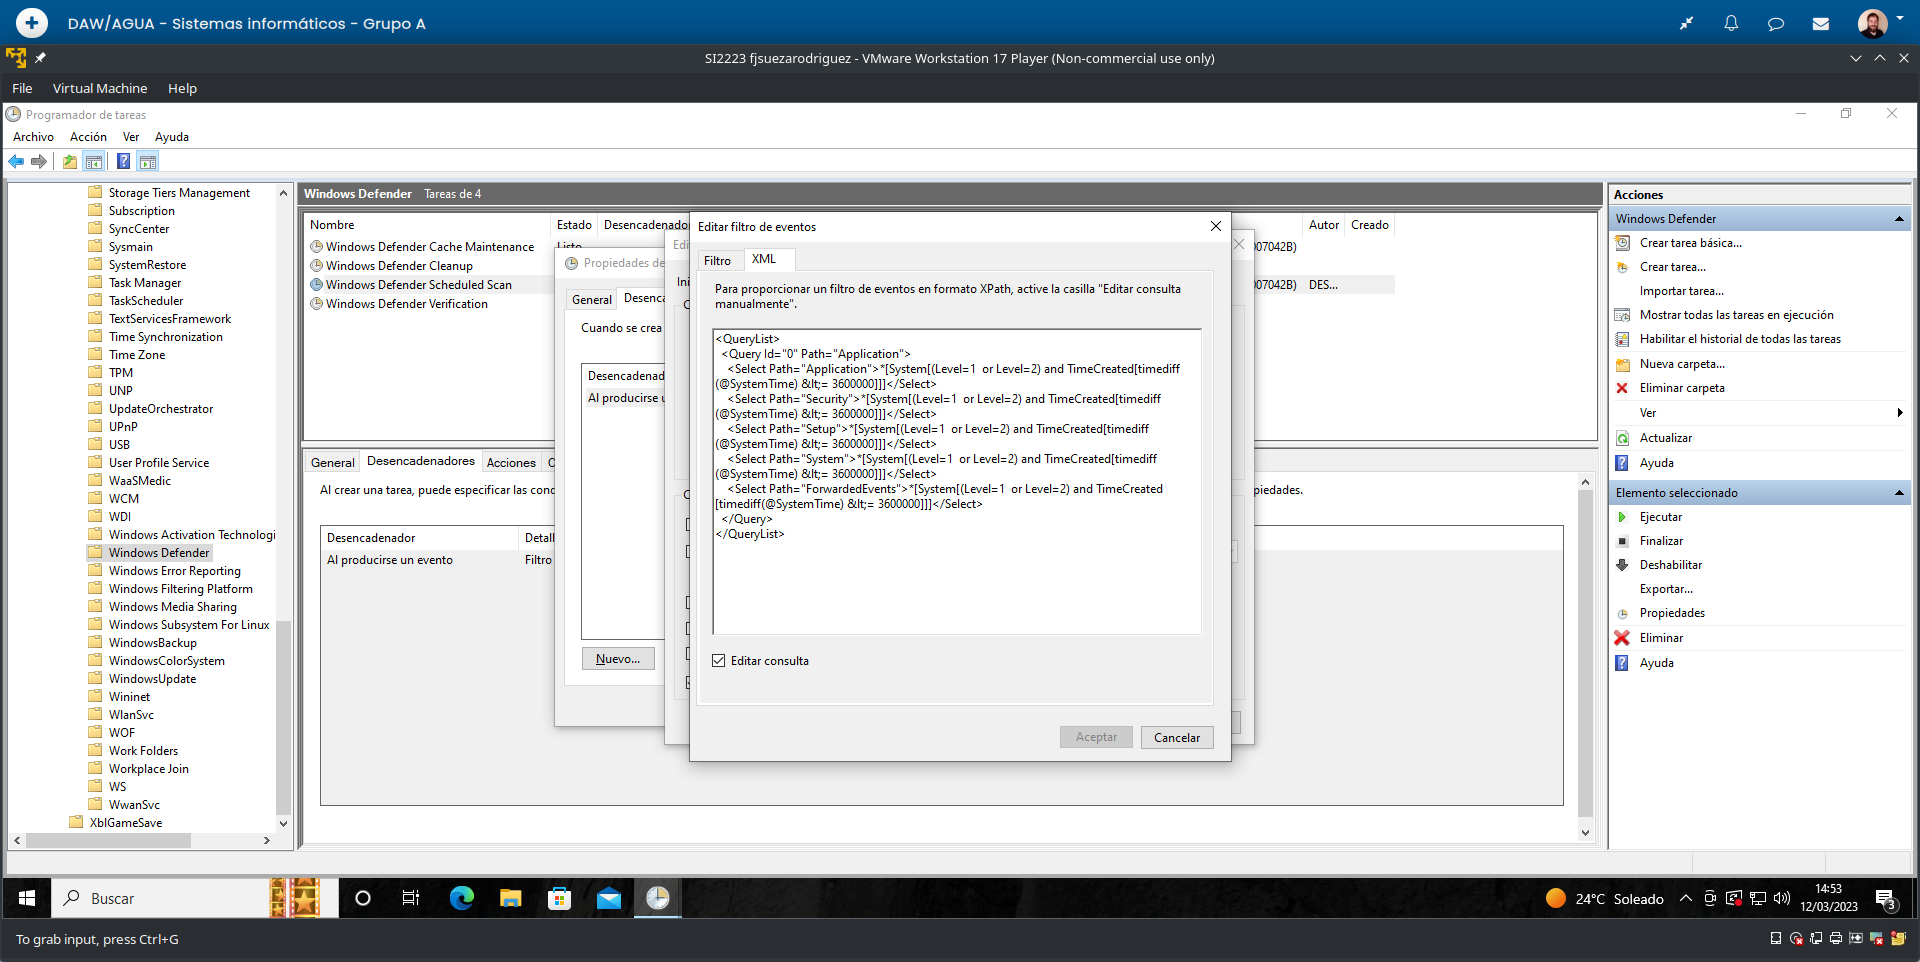
\includegraphics[scale=0.20]{defender-3.png}
        \caption{Filtro de evento creado en formato XML}
    \end{figure}
\end{enumerate}

\subsection{Actividad 6: Windows Update}

\subsubsection{Enunciado}
Realiza una captura de \textbf{Windows Update} que muestre si el sistema está actualizado, con la fecha y hora en la que se realizó la última comprobación. Establece también el horario de \textbf{8:00 a 16:00 horas} como horas activas del equipo y que se muestre una notificación cuando el equipo requiera un reinicio para finalizar una actualización.

\textbf{Capturas}:

\begin{itemize}
    \item Ventana de Windows Update (indica textualmente cómo se accede a dicha ventana).
    \item Información sobre el estado actual del sistema y última actualización.
    \item Introducción de las horas activas del equipo.
    \item Activación de la notificación cuando el equipo requiera un reinicio para finalizar una actualización.
\end{itemize}

\subsubsection{Solución}
Ahora vamos a trabajar con \textbf{Windows Update}, el gestor de actualizaciones de Windows.

\begin{enumerate}
    \item En primer lugar vamos a acceder a la ventana de Windows Update. Esto podemos hacerlo buscando en la barra de búsqueda del sistema el término \textbf{Windows Update} y pulsando en el primer resultado \textbf{Buscar Actualizaciones}, aunque también lo podemos hacer desde la opción \textbf{Actualización y seguridad} del menú \textbf{Configuración}. En la siguiente captura podemos ver la ventana principal de Windows Update.

     \begin{figure}[H]
        \centering
        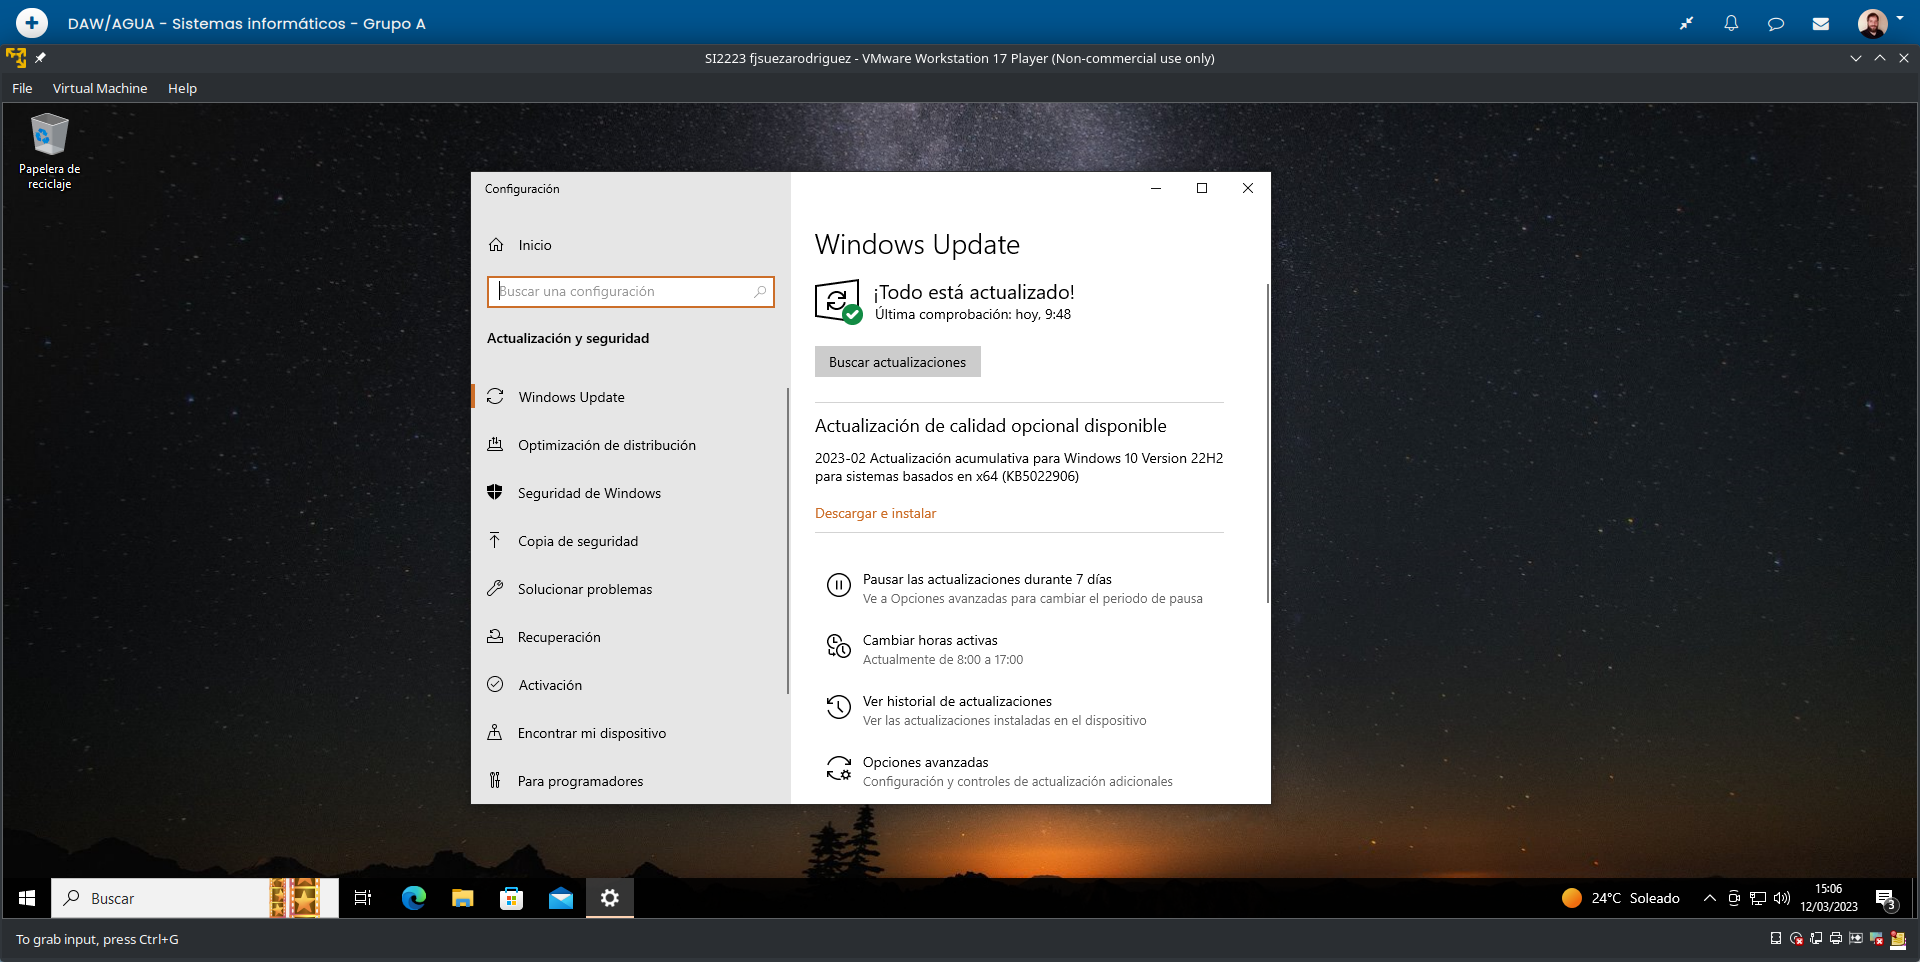
\includegraphics[scale=0.23]{windows-update-1.png}
        \caption{Ventana principal de Windows Update}
    \end{figure}

    \item Para verificar que el sistema esta actualizado, podemos mirar a la parte superior de la captura anterior. Donde podemos observar que el sistema \textbf{esta actualizado} y que la última comprobación se realizo \textbf{hoy a las 9:48}. Vemos también que hay una actualización pendiente, aunque esta es una \textbf{actualización opcional}.

    \textbf{NOTA}: no se incluye captura en este punto ya que es la misma que en el punto 1.

    \item A continuación, vamos a cambiar el \textbf{rango horario }en el que se va a ejecutar Windows Update. Para ello, en la ventana anterior pulsamos en el apartado \textbf{Cambiar horas activas}, donde se nos dará la opción de cambiar el rango horario, como vemos en la siguiente figura.

    \begin{figure}[H]
        \centering
        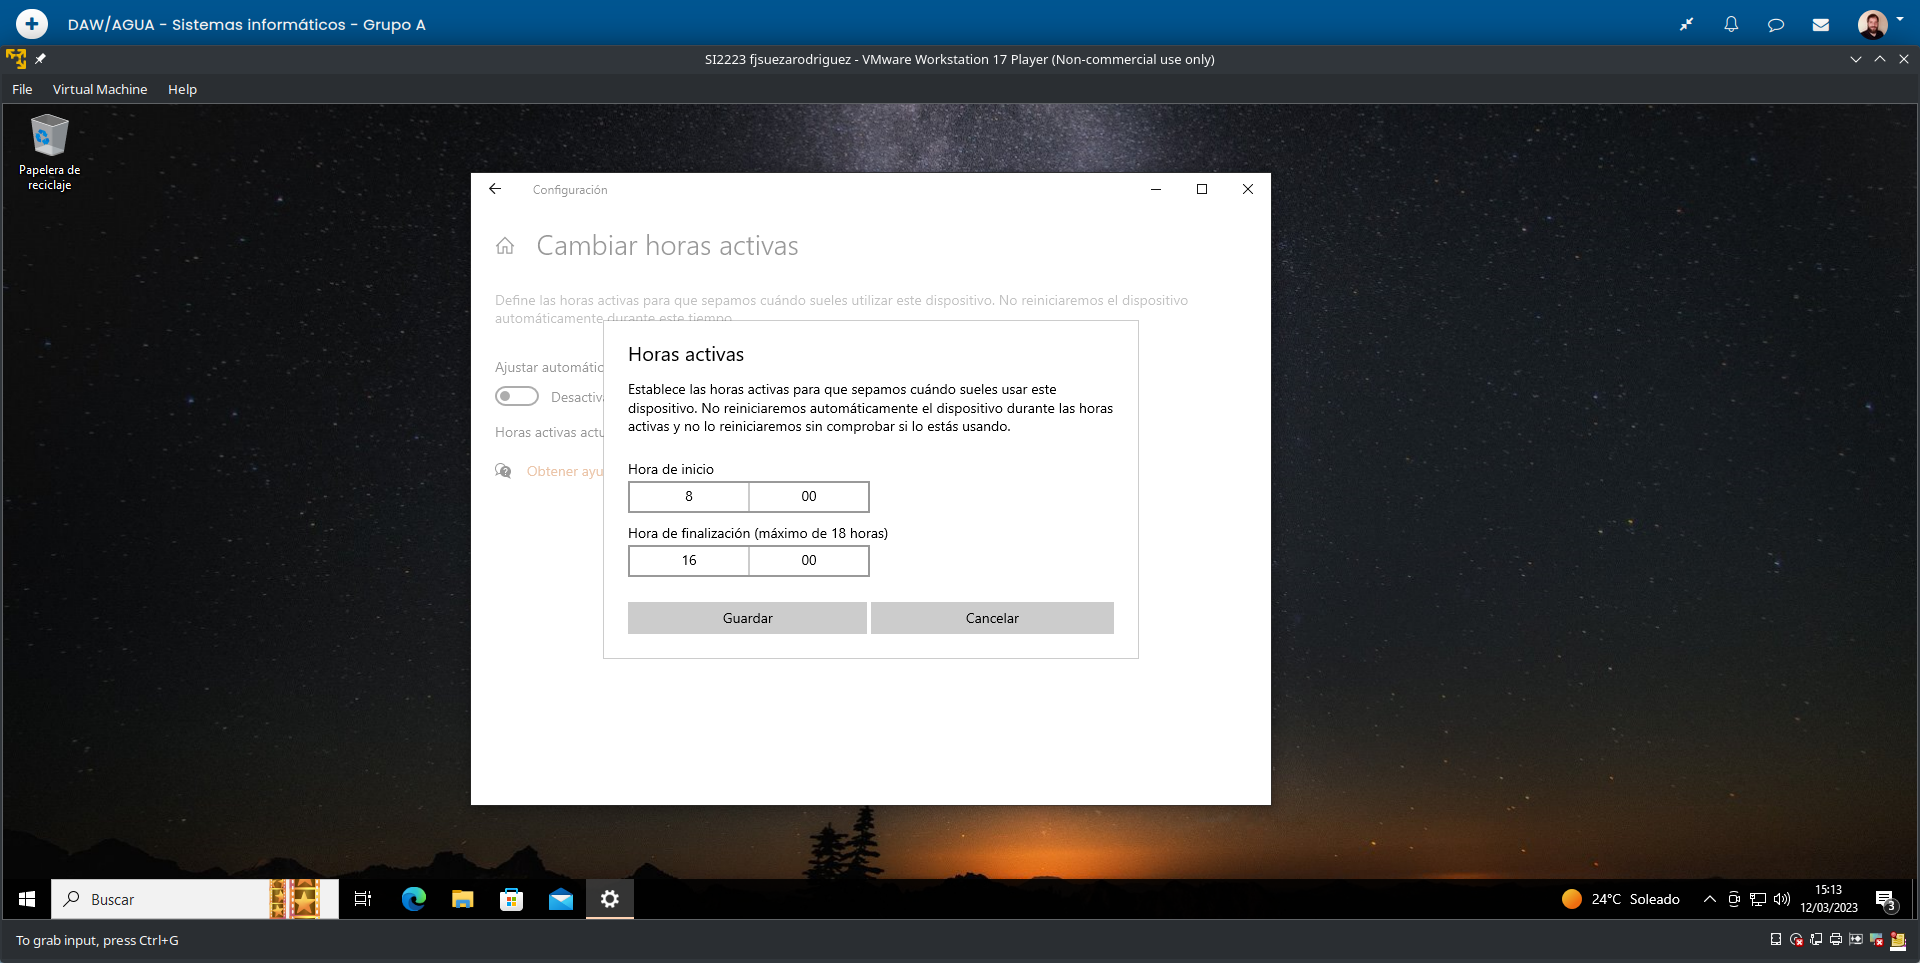
\includegraphics[scale=0.23]{windows-update-2.png}
        \caption{Cambio de rango horario para la ejecución de Windows Update}
    \end{figure}

    \item Por último, vamos a activar la \textbf{Notificación de Actualización}, para que nos notifique cada vez que el sistema necesita reiniciarse para realizar una actualización. Esta opción la encontramos en el apartado \textbf{Opciones avanzadas}, donde podemos activarla.

    \begin{figure}[H]
        \centering
        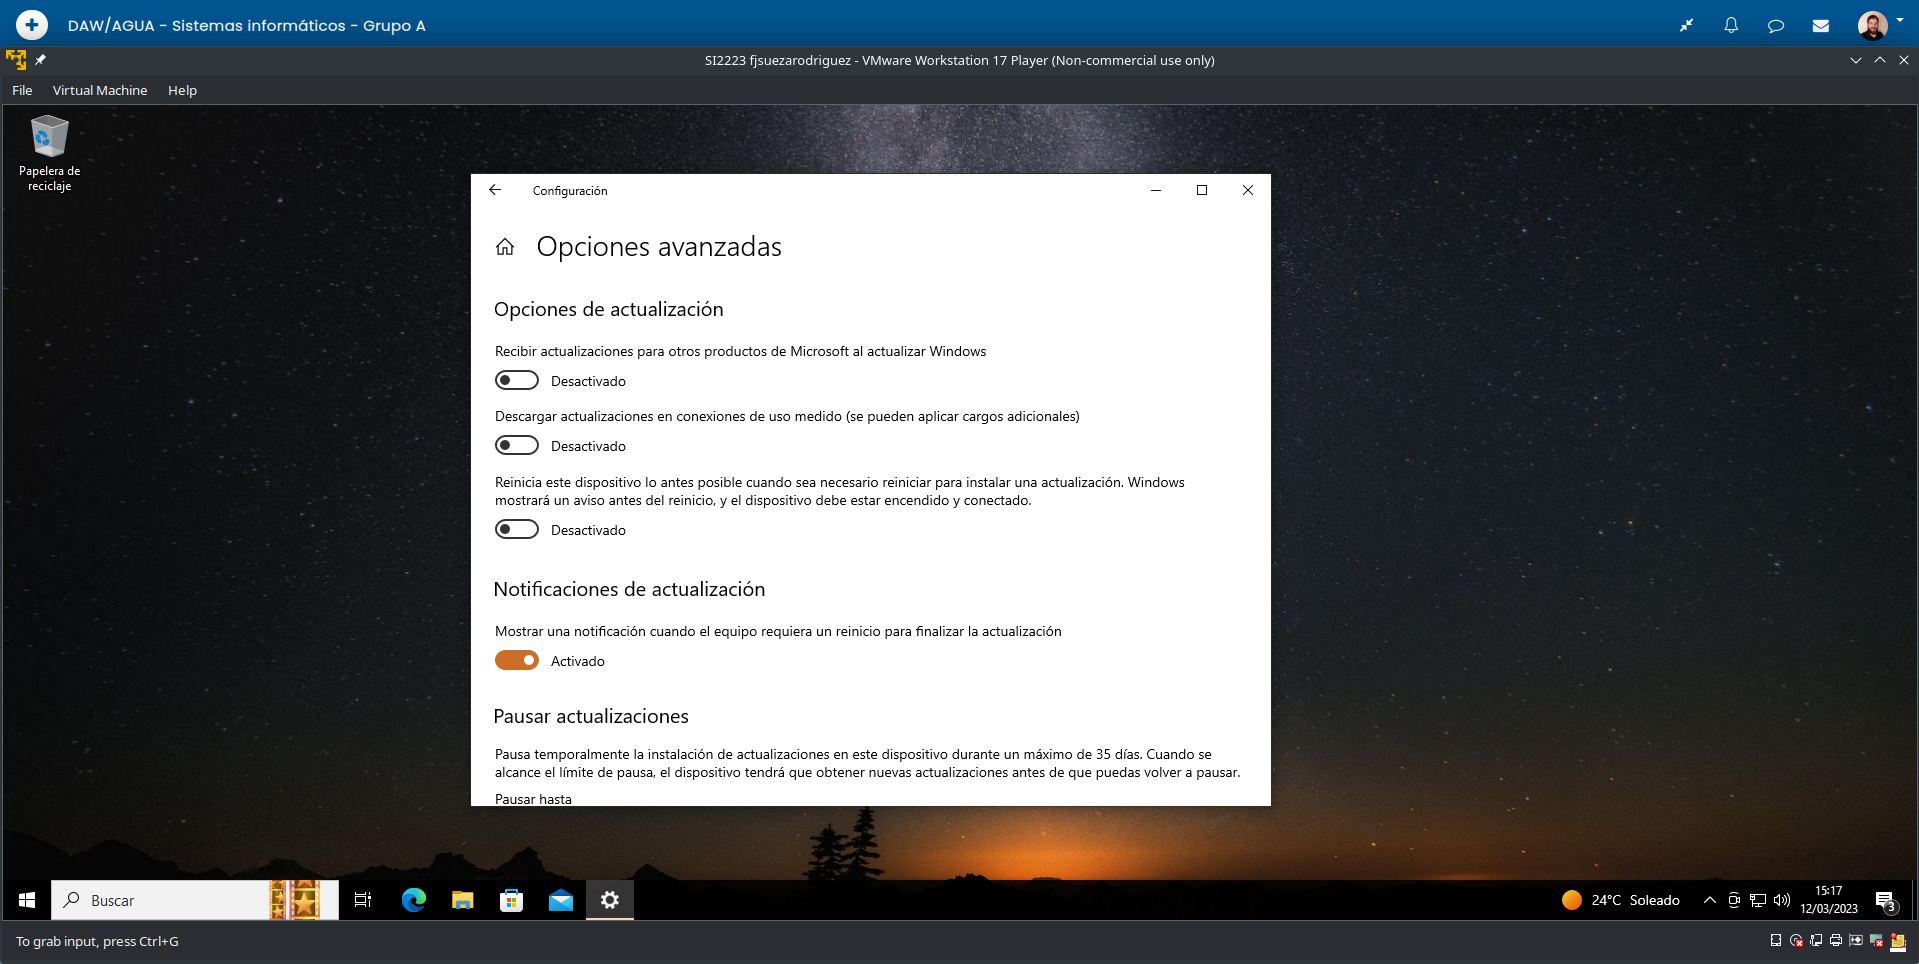
\includegraphics[scale=0.23]{windows-update-3.png}
        \caption{Activación de notificaciones de Windows Update}
    \end{figure}
\end{enumerate}

\subsection{Actividad 7: Monitor de Rendimiento}

\subsubsection{Enunciado}
Antes de empezar debes consultar la sección ``\textbf{Conocimiento Previo}'' (al final de esta página).

La actividad consiste en crear un nuevo conjunto recolector de datos dentro del Monitor de rendimiento, que tendrá como nombre recolector\_InicialNombreApellidos. Usa la plantilla de creación ``System Diagnostics'' con la que se recogerán todas las estadísticas de rendimiento posibles. Establece como usuario del recolector el usuario creado al instalar el sistema (con permisos de Administrador).

Inicia manualmente el conjunto recolector recién creado y detenlo después de 1 minuto.

Para la 2ª ejecución del recolector deberás realizar una prueba de estrés al sistema (abre varias instancias del navegador, descarga un compresor de archivos tipo WinRAR o 7-zip, comprime/descomprime carpetas con bastante volumen, reproduce videos 4k, descarga videos pesados y usa un reproductor para visualizarlos, abre tantos programas como puedas, ...).

Comenta las diferencias que encuentras en los 2 informes generados en cada ejecución: ¿Qué contadores del sistema se han visto más afectados al estresar el equipo? Relaciona contadores con la carga de trabajos realizada. ¿Hay algún cuello de botella crítico en la configuración actual de tu máquina virtual que podrías modificar? Valora posibles soluciones.

\textbf{Capturas}:
\begin{itemize}
    \item Ventana donde se muestra el Monitor de rendimiento con el colector creado ejecutándose.
    \item Ventanas donde se muestren cada uno de los informes resultado, teniendo desplegados los epígrafes ``Rendimiento'' y ``Advertencias'' (si las hubiera) .
\end{itemize}

\subsubsection{Solución}

En esta actividad vamos a analizar el rendimiento del sistema usando el \textbf{Monitor del Sistema}, para lo que vamos a crear un nuevo recolector de datos y realizar 2 análisis, uno con el sistema en reposo y otro estresándolo.

\begin{enumerate}
    \item En primer lugar hemos creado el recolector de datos, llamado \textbf{recolector\_fjsuezarodriguez} y usando la plantilla \textbf{System Diagnostics}. En la siguiente captura, podemos ver el recolector creado ejecutándose.

    \begin{figure}[H]
        \centering
        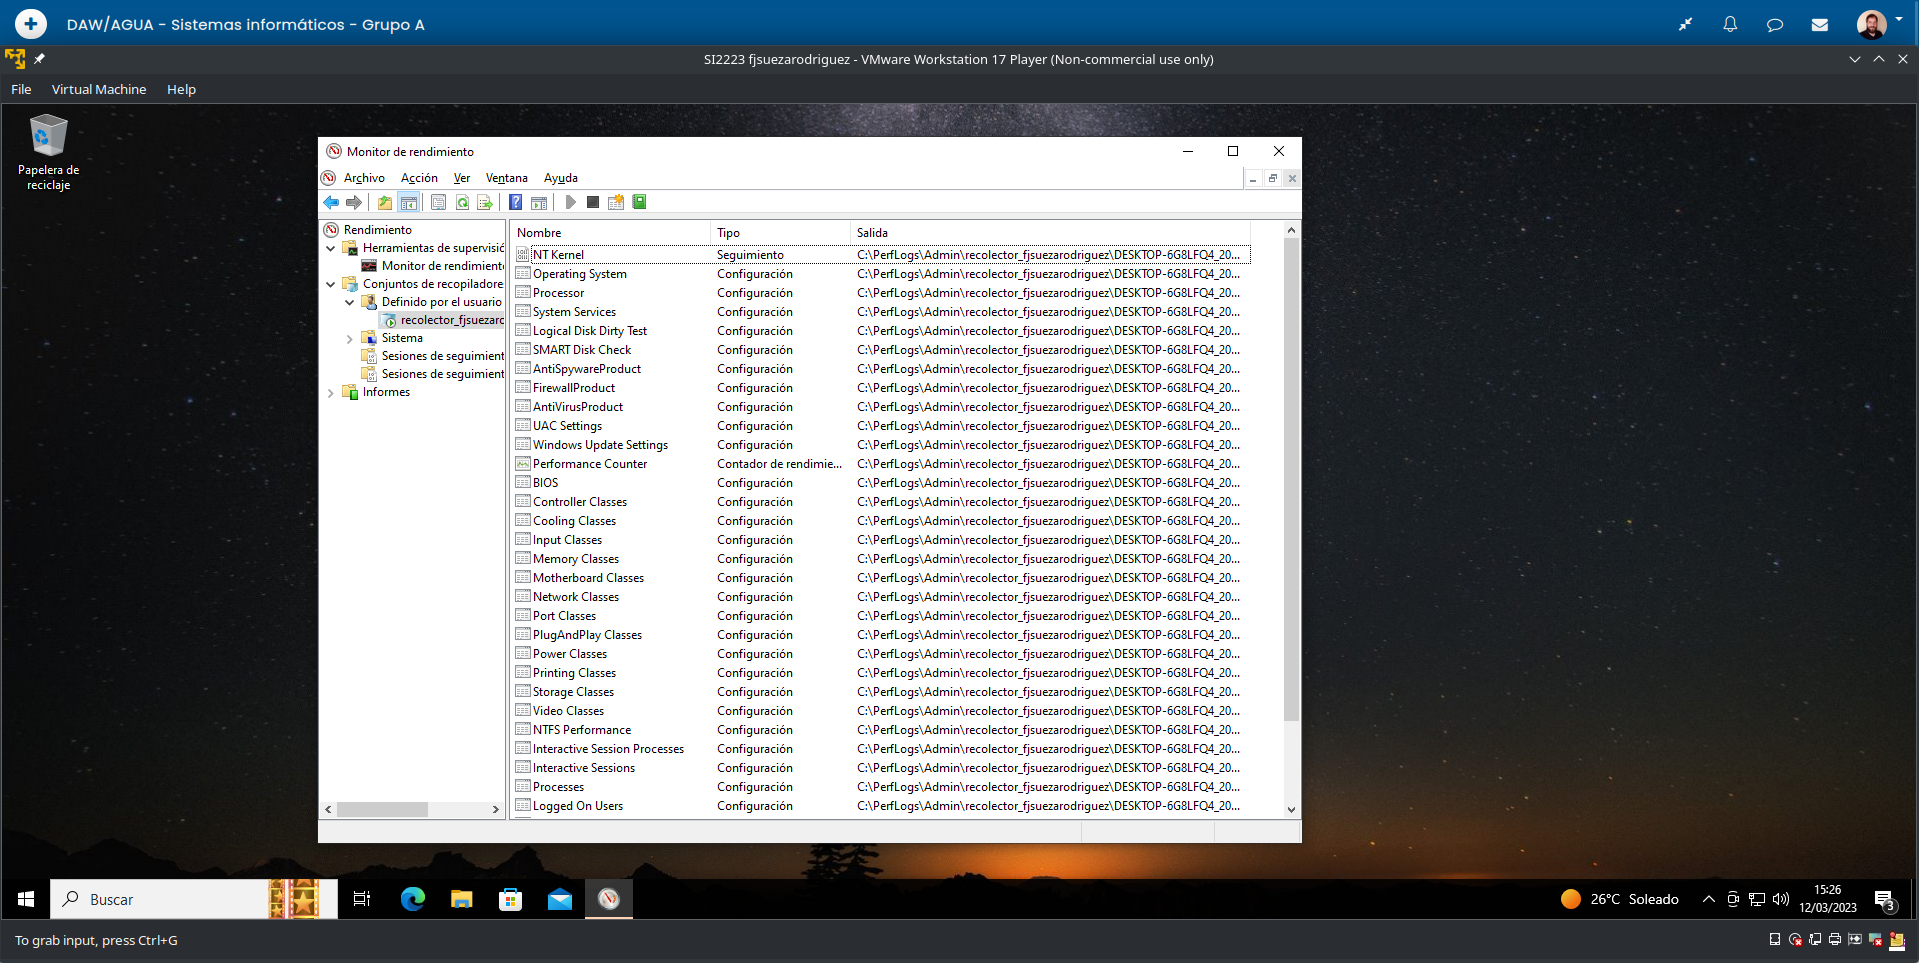
\includegraphics[scale=0.23]{recopilador-1.png}
        \caption{Recolector de datos creado en ejecución}
    \end{figure}

    \item Una vez realizados los dos análisis, podemos ver los resultados.

    En el \textbf{primer análisis}, los resultados han sido satisfactorios en tema de \textbf{rendimiento}, aunque el sistema nos ha lanzado varias advertencias, a modo de información sobre la \textbf{evaluación baja} de la \textbf{CPU}, los \textbf{gráficos} y el \textbf{disco duro}. También se nos informa de que la memoria RAM es \textbf{muy insuficiente}.

    Esto es debido a las propias limitaciones del \textbf{Host}, ya que solo la MV tiene asignados solo \textbf{2 GB de RAM} y esta usando \textbf{2 núcleos}, de los 4 que tiene el sistema Host. Además, la gráfica es una Vega 8 integrada, que no es la mejor para utilizarla en juegos. En la siguiente captura, podemos ver el resultado del análisis.

    \begin{figure}[H]
        \centering
        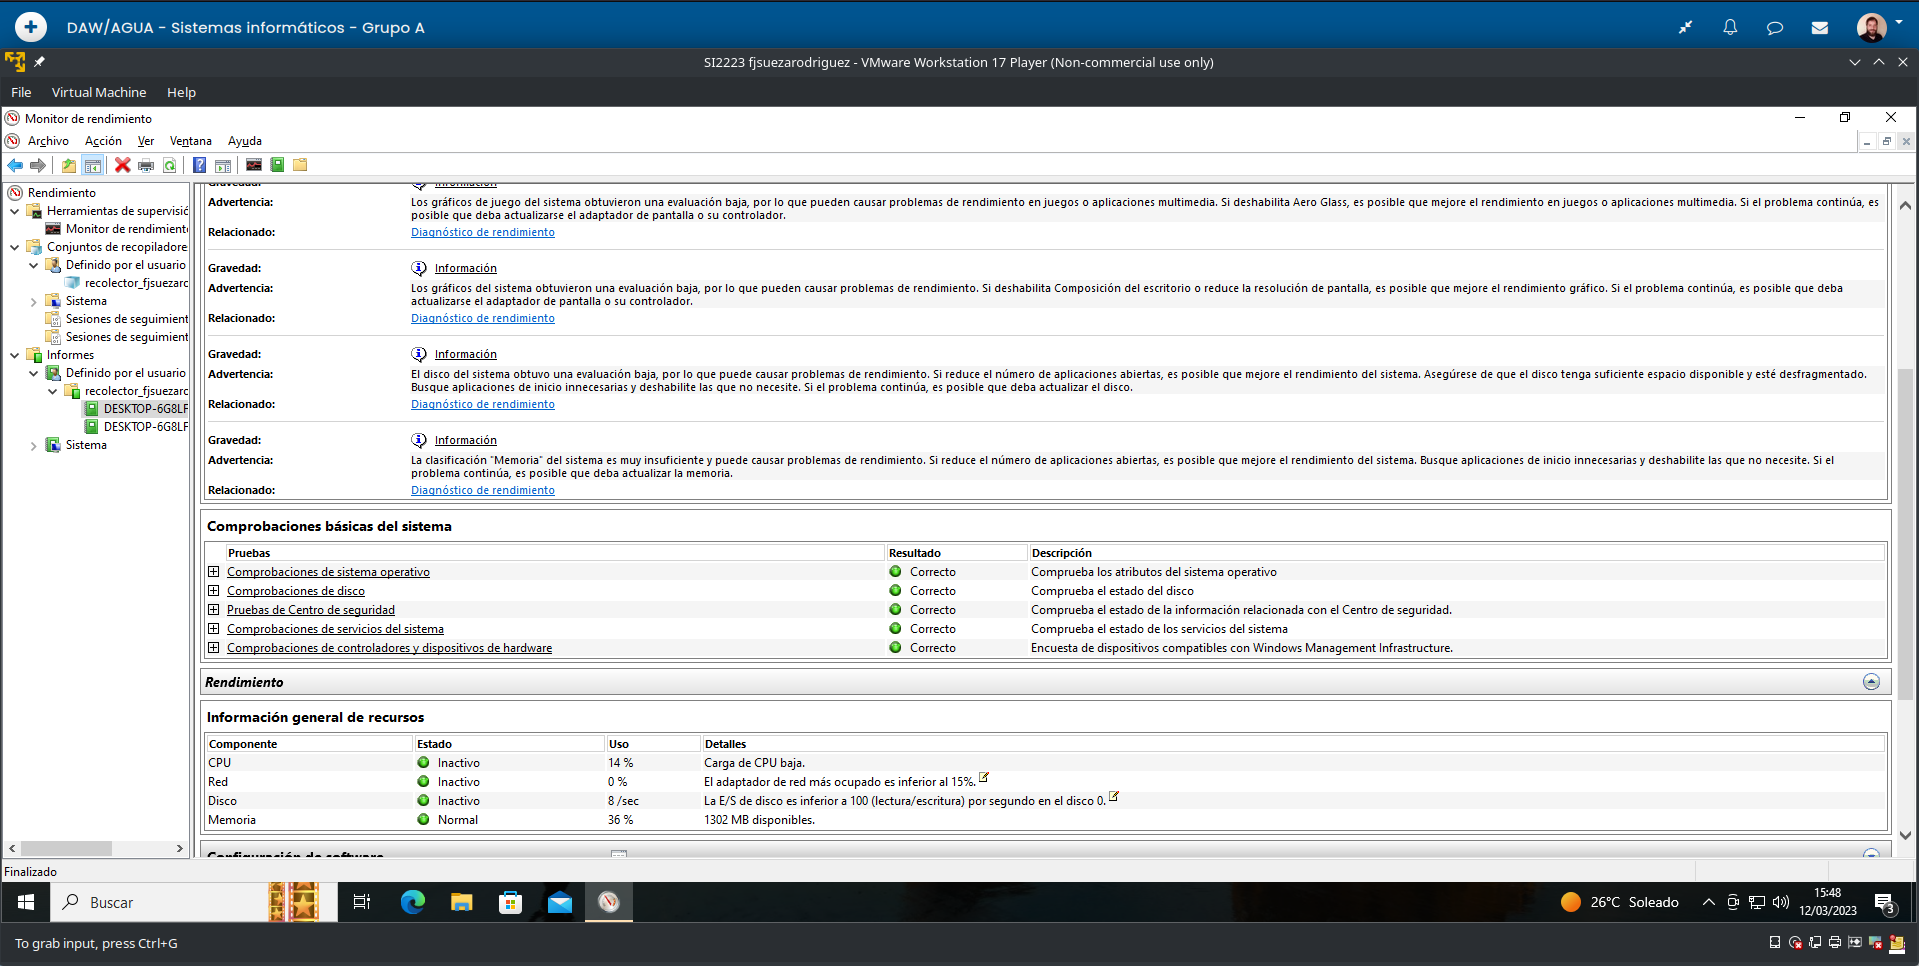
\includegraphics[scale=0.23]{recopilador-2.png}
        \caption{Informe del primer análisis de rendimiento}
    \end{figure}

    \item Tras el primer análisis, hemos realizado un segundo intentando estresar el sistema, para lo que hemos abierto varias aplicaciones, varias pestañas en Edge, etc... El \textbf{resultado es muy similar}, salvo que en este segundo análisis la \textbf{CPU} ha salido con una carga muy elevada, en concreto del \textbf{90\%}, como vemos en la siguiente captura.

    \begin{figure}[H]
        \centering
        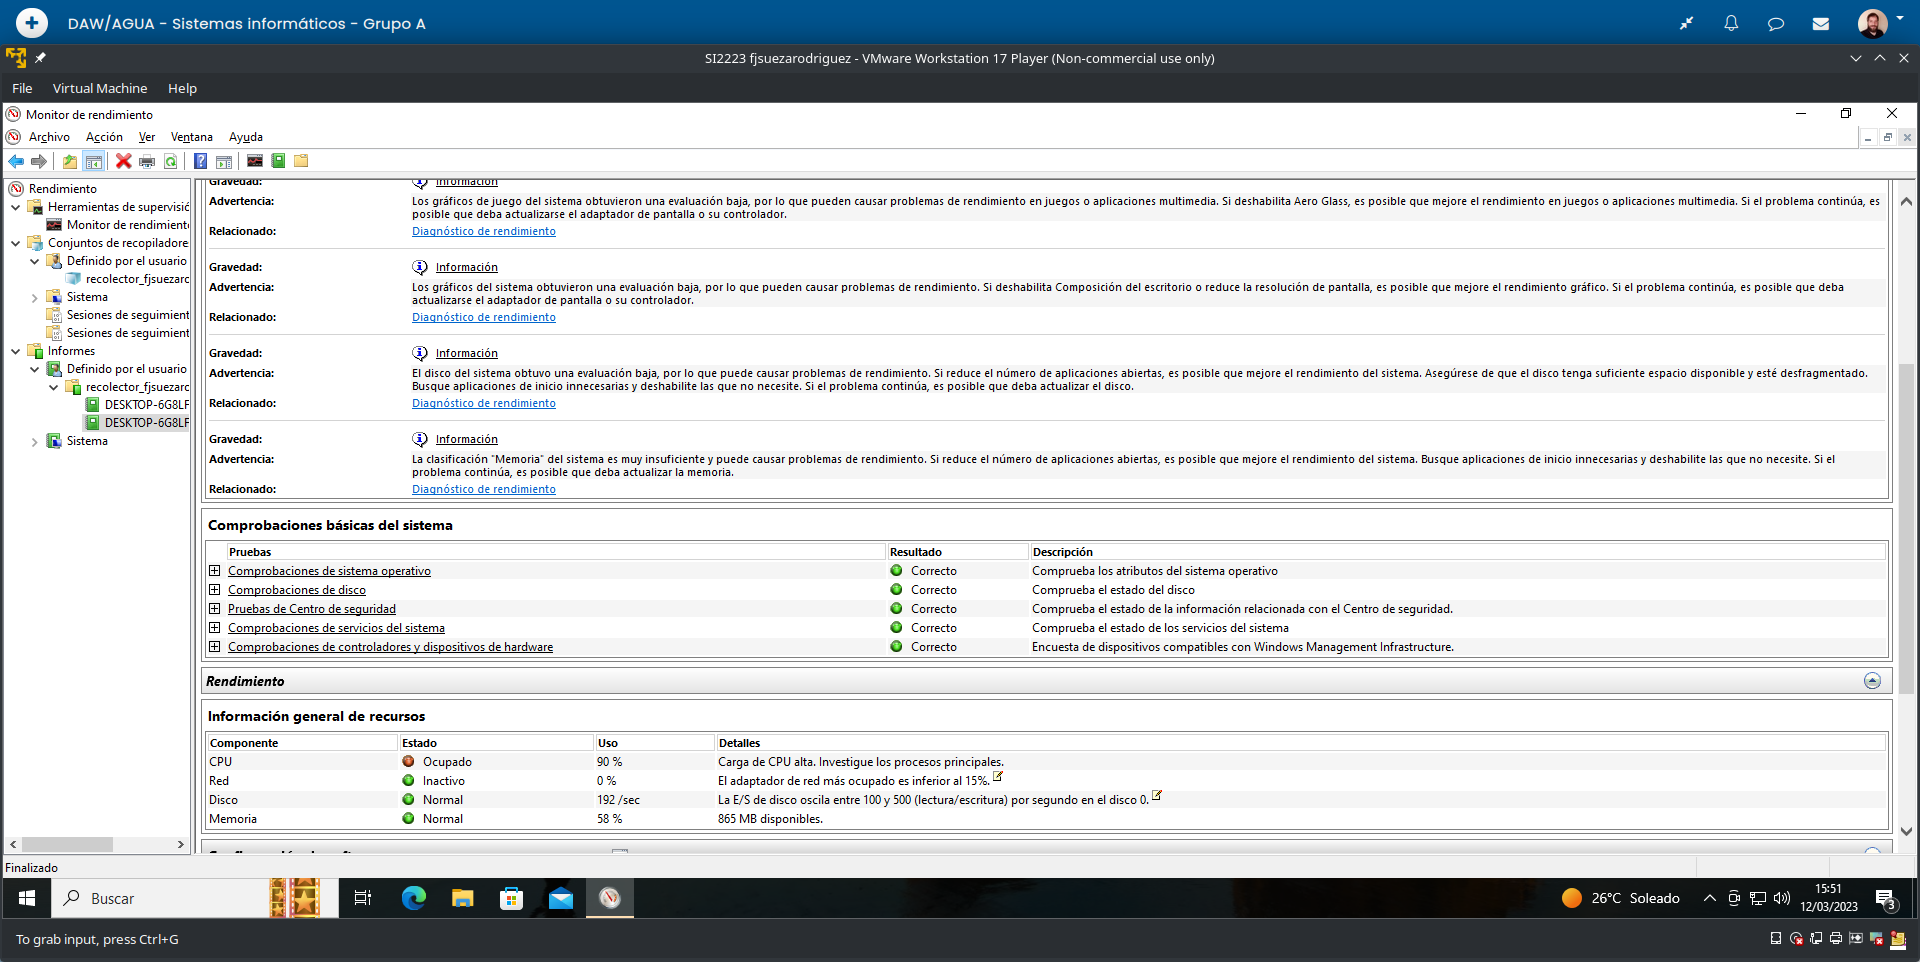
\includegraphics[scale=0.23]{recopilador-3.png}
        \caption{Informe del segundo análisis de rendimiento}
    \end{figure}
\end{enumerate}

Por último, \textbf{comentar los análisis}, aunque como ya hemos dicho estas advertencias se deben a las \textbf{limitaciones de host}, por lo que la única solución sería, o bien \textbf{actualizar el hardware} del sistema anfitrión, o intentar \textbf{asignar más recursos} a la máquina virtual a ver si así se soluciona alguno de los problemas de \textbf{performance}.

\subsection{Actividad 8: Servicios}
\subsubsection{Enunciado}
Inicia el servicio ``\textbf{Cliente web}'' y detiene el servicio ``\textbf{Audio de Windows}'' (una vez hecha la captura solicitada, vuelve a iniciar el servicio).

\textbf{Capturas}:
\begin{itemize}
    \item Ventana donde se muestran los servicios (indica textualmente cómo se accede a dicha ventana).
    \item Activación/Inicio del servicio ``Cliente web''.
    \item Captura donde se vea el icono de volumen en rojo en la barra de estado, indicando que el servicio ``Audio de Windows'' no está activo.
\end{itemize}

\subsubsection{Solución}
En esta actividad vamos a gestionar los \textbf{servicios locales} de Windows 10. En concreto, vamos a \textbf{habilitar el cliente web} y vamos a \textbf{deshabilitar} el servicio \textbf{audio de windows}.

\begin{enumerate}
    \item En primer lugar tenemos que abrir el gestor de servicios. Si buscamos en la barra de búsqueda de Windows el termino \textbf{servicios} nos aparecerá como el primer resultado. Pulsando en éste, se nos abrirá el \textbf{gestos de servicios}.

    \begin{figure}[H]
        \centering
        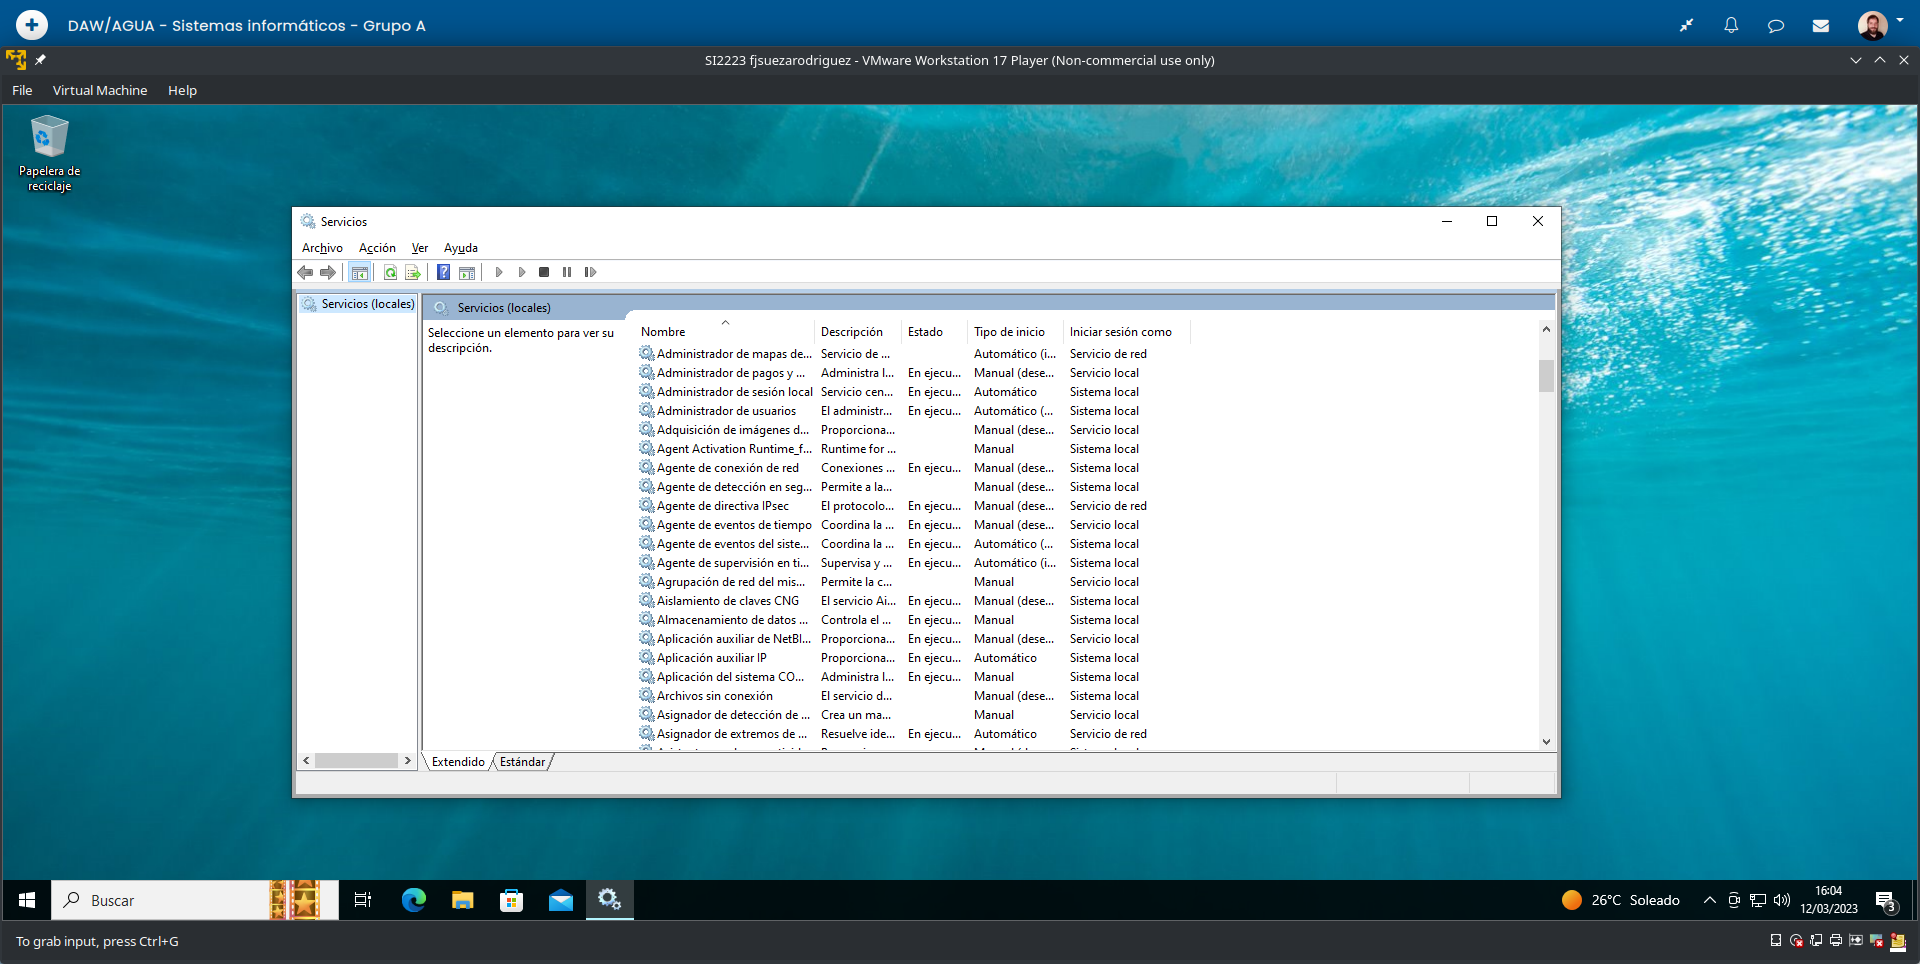
\includegraphics[scale=0.20]{servicios-1.png}
        \caption{Gestor de servicios de Windows 10}
    \end{figure}

    \item A continuación, vamos a activar el servicio \textbf{Cliente Web}. Para ello, buscamos el servicio en la lista y a continuación en \textbf{Iniciar} en la ventana que se nos abrirá.

    \begin{figure}[H]
        \centering
        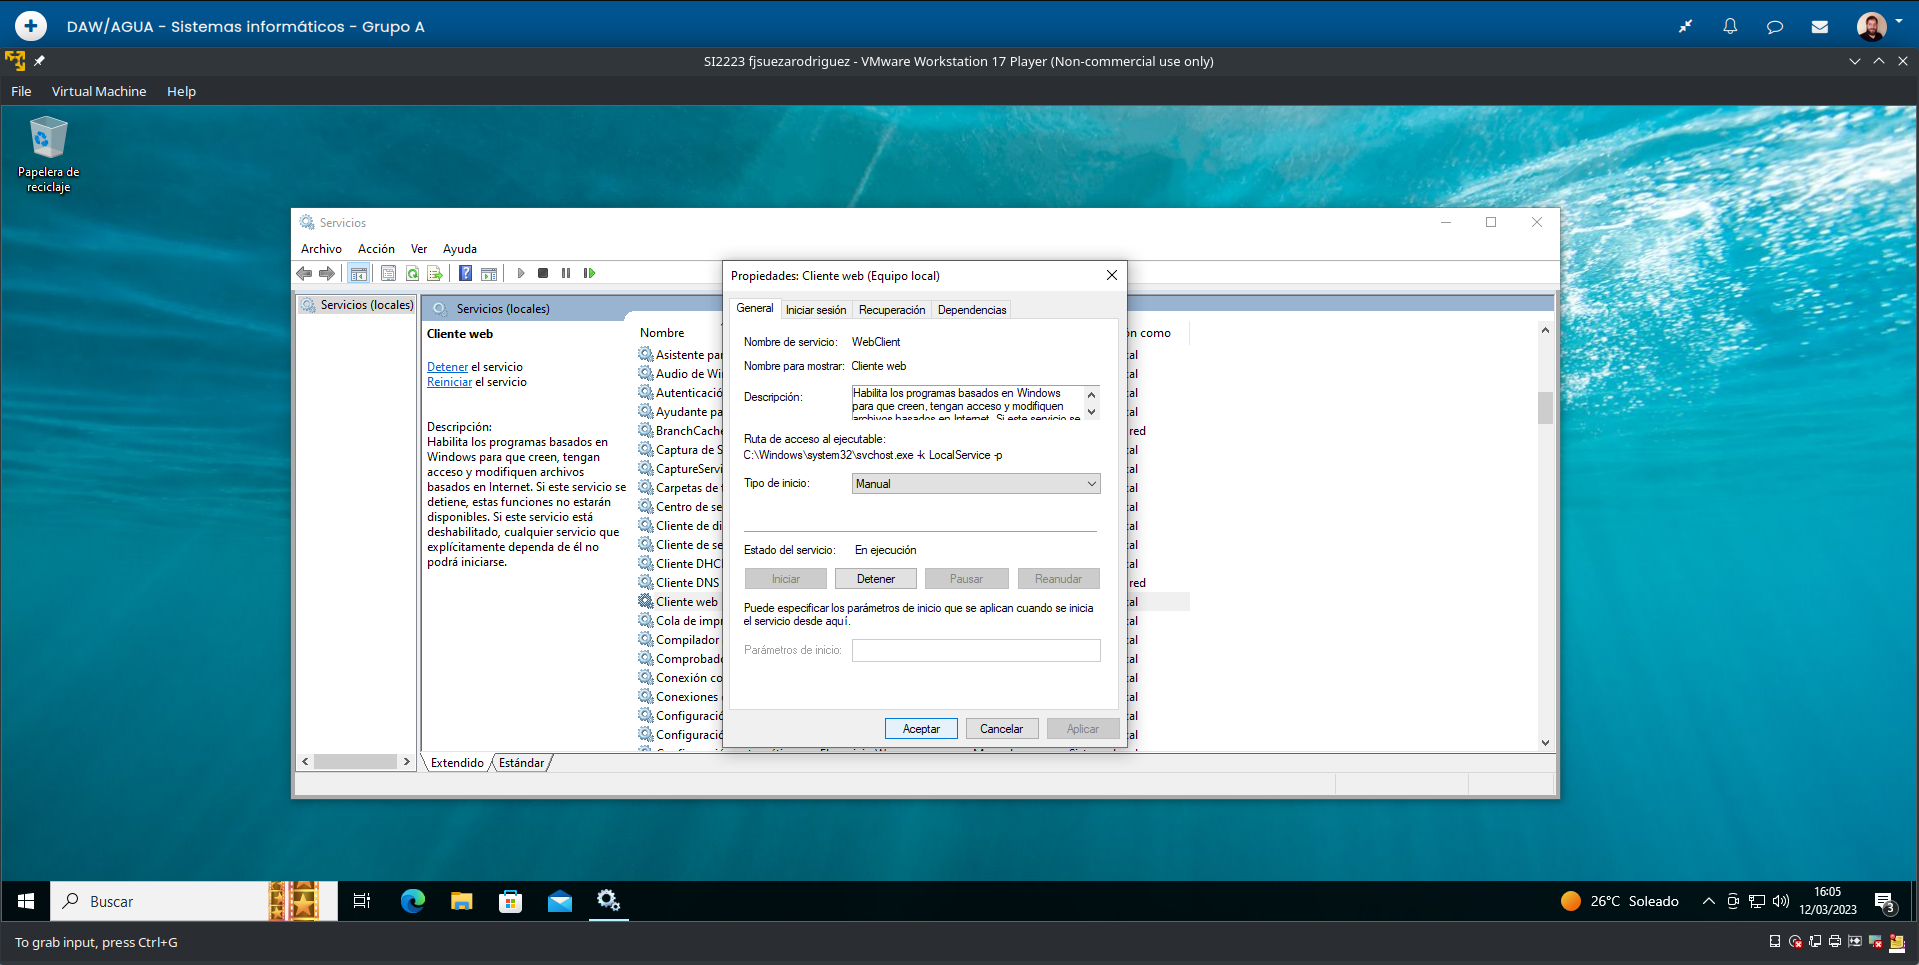
\includegraphics[scale=0.20]{servicios-2.png}
        \caption{Inicialización del Cliente Web}
    \end{figure}

    \item Por último, vamos a deshabilitar el servicio \textbf{Audio de Windows}. Para ello, al igual que en el punto anterior, buscamos el nombre del servicio en la lista, solo que ahora pulsaremos en la opción \textbf{Detener}. En la siguiente captura, se muestra como el icono de volumen aparece en rojo.

    \begin{figure}[H]
        \centering
        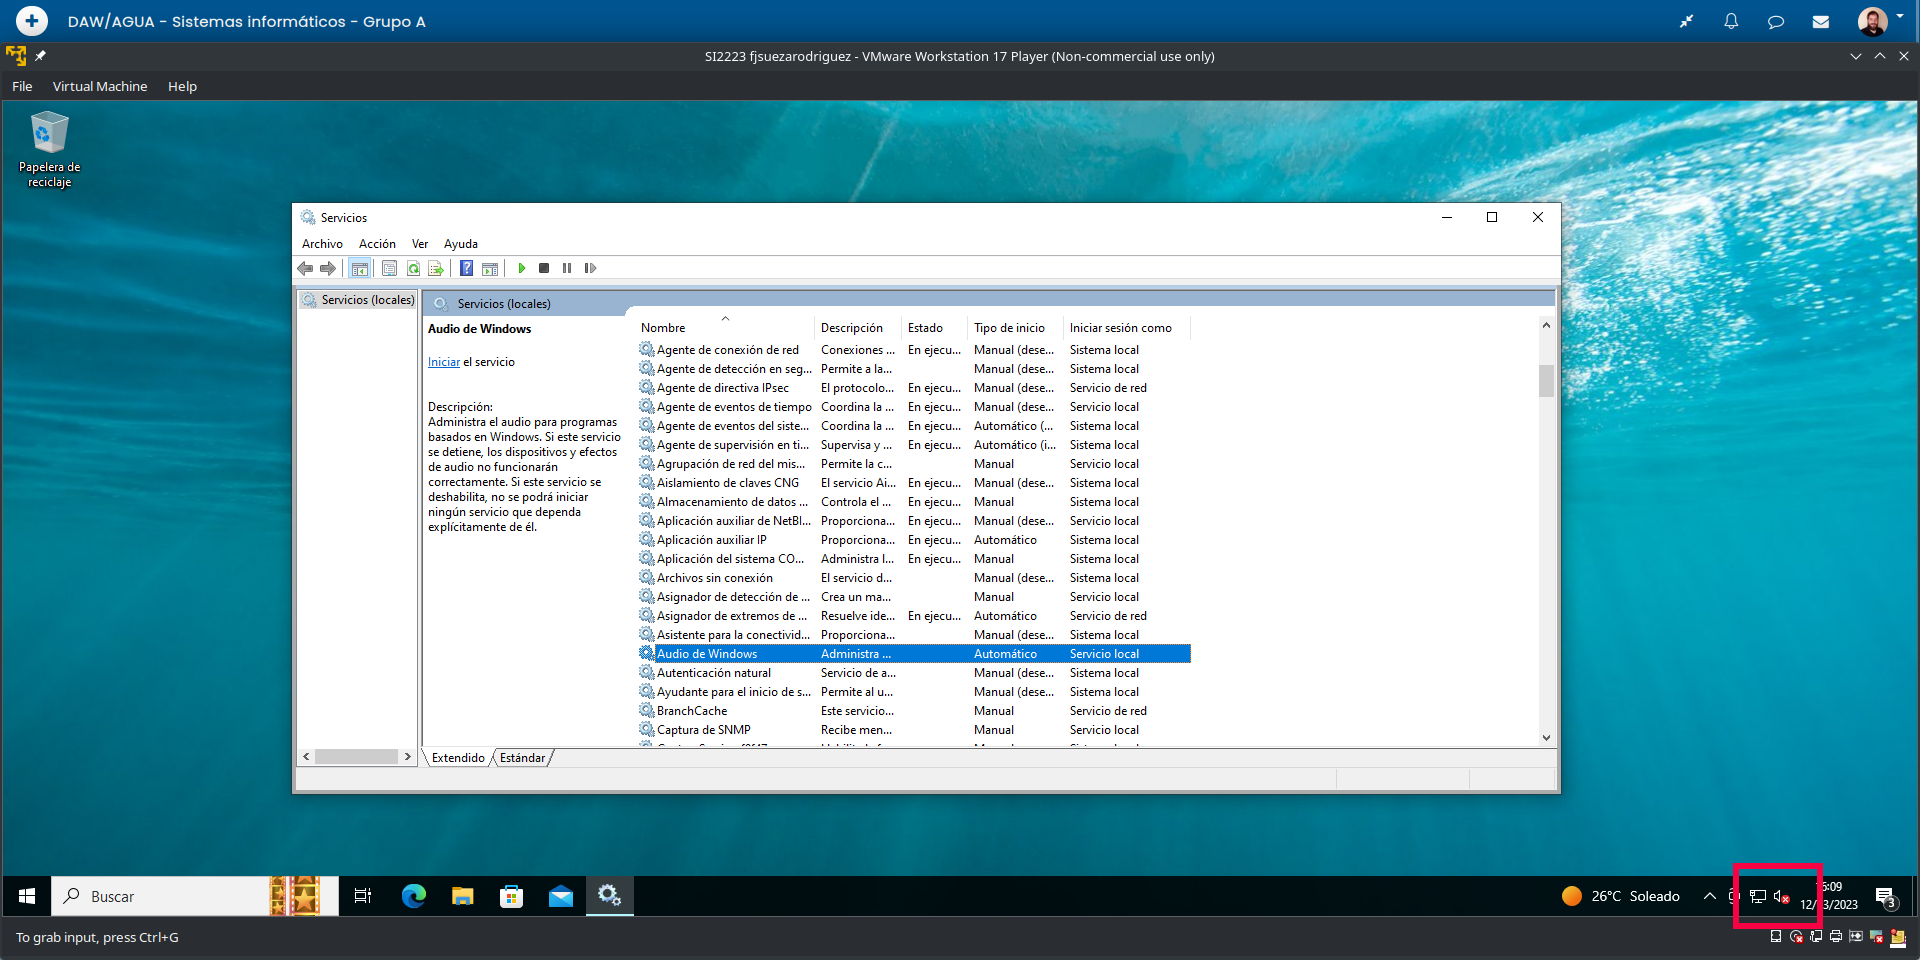
\includegraphics[scale=0.20]{servicios-3.png}
        \caption{Audio de Windows deshabilitado}
    \end{figure}
\end{enumerate}

\subsection{Actividad 9: Puntos de Restauración}
\subsubsection{Enunciado}
Los puntos de restauración sirven para volver a configuraciones guardadas del sistema previas a alguna modificación o instalación de programas.

Crea un punto de restauración con el nombre SI2223InicialesApellido1Apellido2 (por ejemplo, para ``José Luis Pérez Puertas'' sería ``SI2223 jlperezpuertas''). Después cambia el tema de Windows por otro que sea lo más distinto posible al que tenías. A continuación restaura el sistema y comprueba que el cambio de tema realizado ha quedado sin efecto.

\textbf{Capturas}:

\begin{itemize}
    \item Ventana donde se crea un punto de restauración y se aprecie la hora del sistema (indica textualmente cómo se accede a dicha ventana).
    \item Ventana con el nuevo tema configurado y se aprecie la hora.
    \item Ventana después de la restauración en la que se aprecie la hora y el tema previo.
\end{itemize}

\subsubsection{Solución}
En este ejercicio vamos a establecer un \textbf{punto de restauración} del sistema, lo que nos permitirá volver a un configuración anterior en caso de que el sistema operativo sufra algún fallo.

\begin{enumerate}
    \item En primer lugar, vamos a abrir la aplicación para establecer un punto de restauración. Nosotros hemos accedido buscando el termino \textbf{punto de restauración} en la \textbf{barra de búsqueda} y pulsando en el primer resultado, \textbf{Crear punto de restauración}, ya que esto nos lleva directamente a la pestaña \textbf{Protección del sistema}, donde podemos crearlo. Aunque también podemos acceder desde \textbf{Panel de Control ---> Sistema y Seguridad ---> Sistema}.

    En esta ventana, primero, deberemos seleccionar la unidad sobre la que queremos crear el punto de restauración, pulsar en \textbf{Configurar}, y activar la protección del sistema. De otro modo, no nos permitirá crear un punto de restauración. Una vez hecho esto, pulsamos en crear para crear un nuevo punto de restauración e introducimos el nombre que queramos.

    \begin{figure}[H]
        \centering
        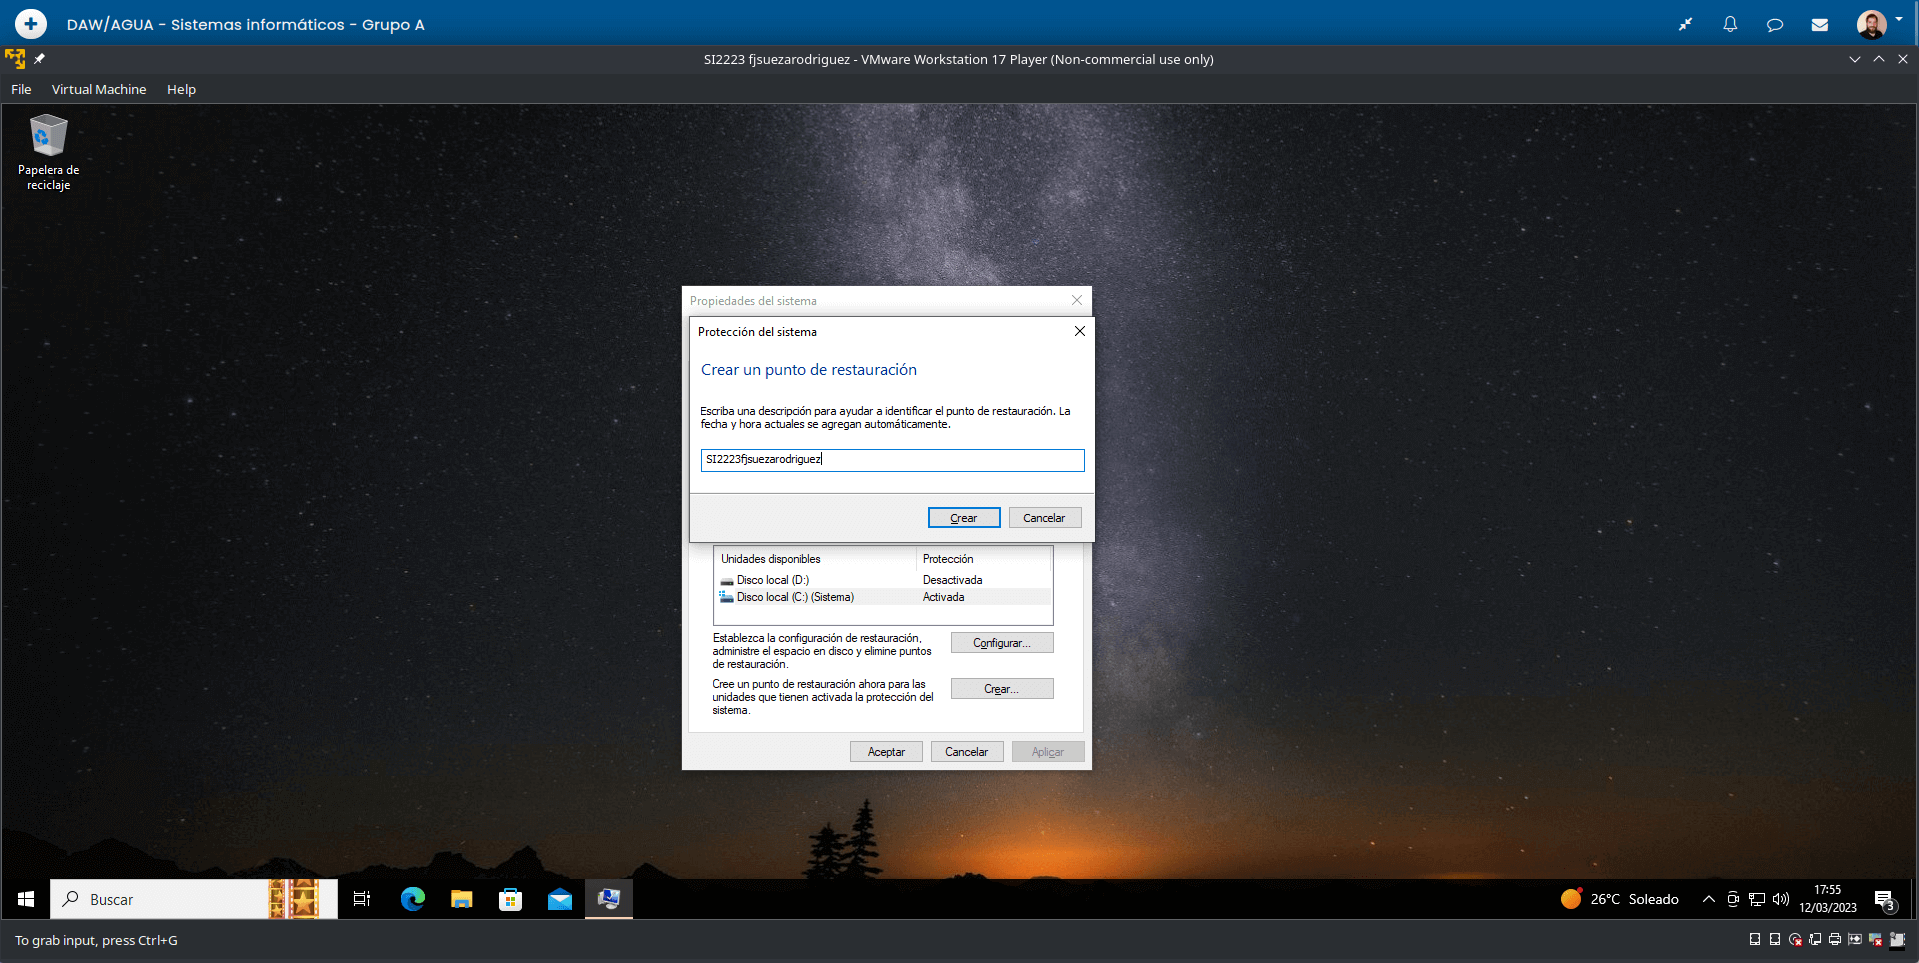
\includegraphics[scale=0.16]{restauracion-1.png}
        \caption{Creación de un punto de restauración}
    \end{figure}

    \item A continuación hemos cambiado el tema de escritorio a Windows (claro), como se puede ver en la siguiente imagen.

    \begin{figure}[H]
        \centering
        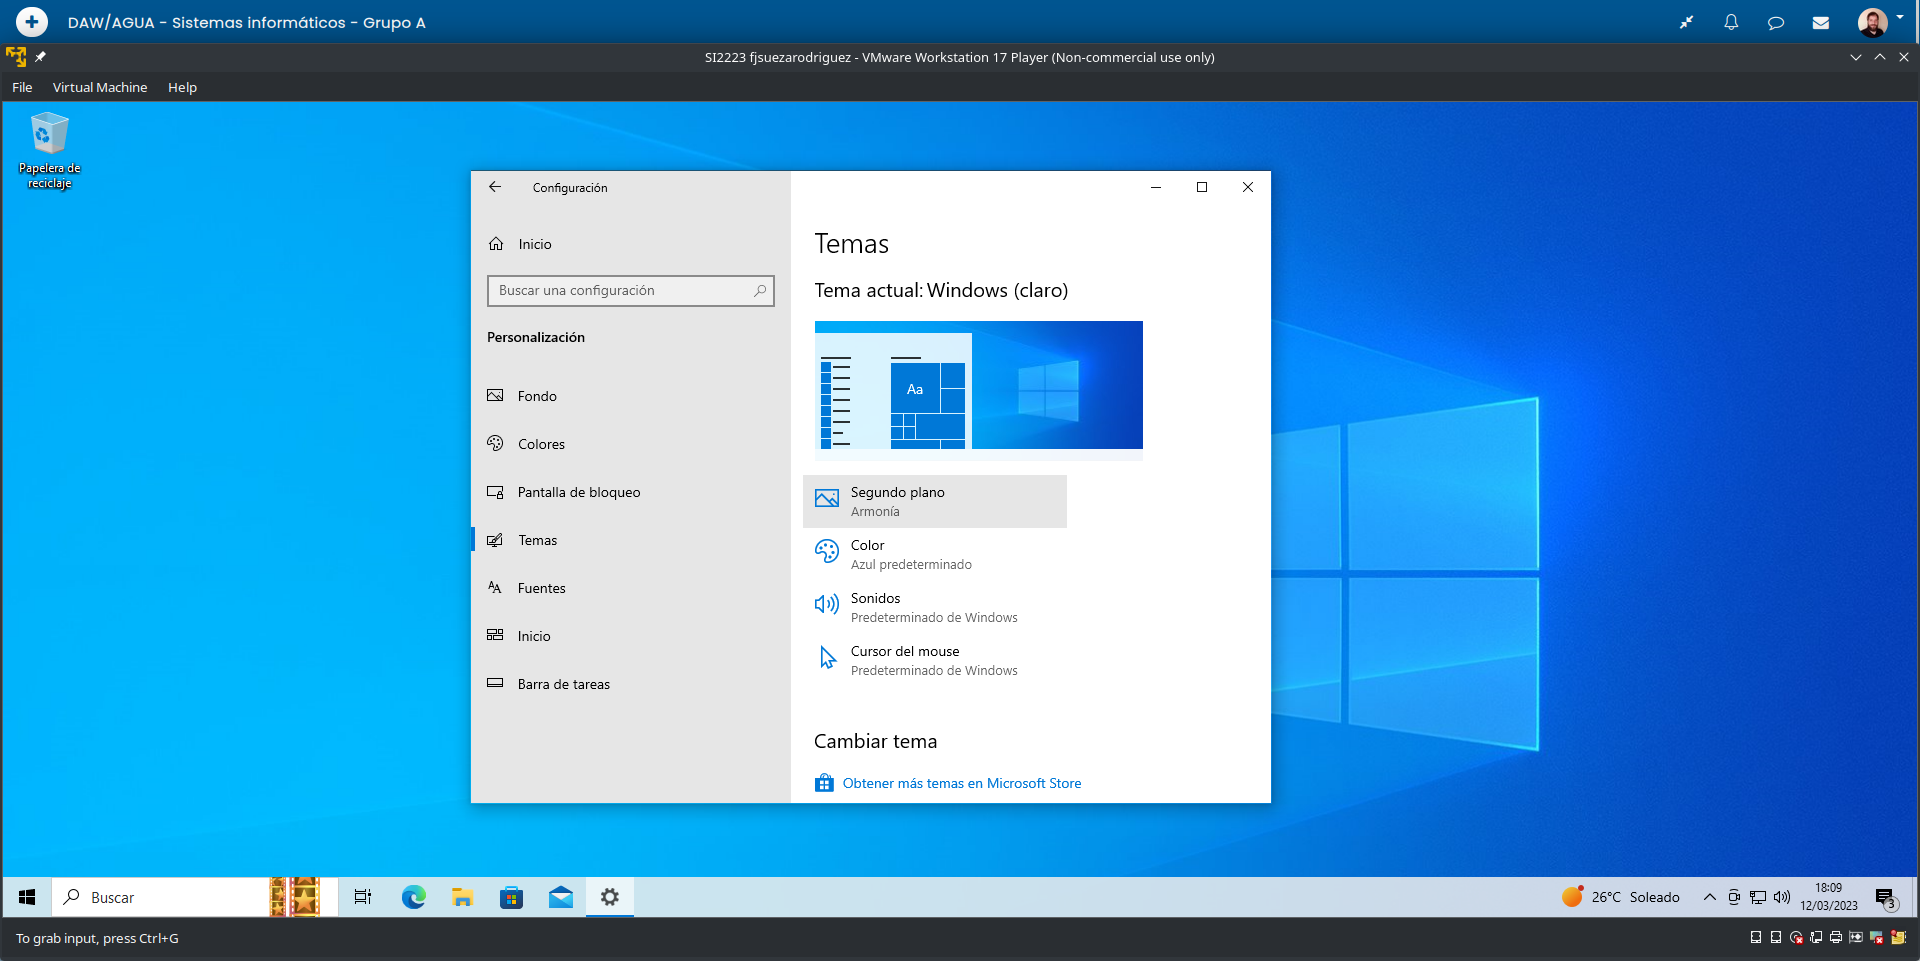
\includegraphics[scale=0.21]{restauracion-2.png}
        \caption{Tema cambiado a Windows(claro)}
    \end{figure}

    \item Por último, hemos realizado la restauración del sistema, volviendo a los valores que teníamos en el momento que se creo el punto de restauración, incluyendo el tema de escritorio.

    \begin{figure}[H]
        \centering
        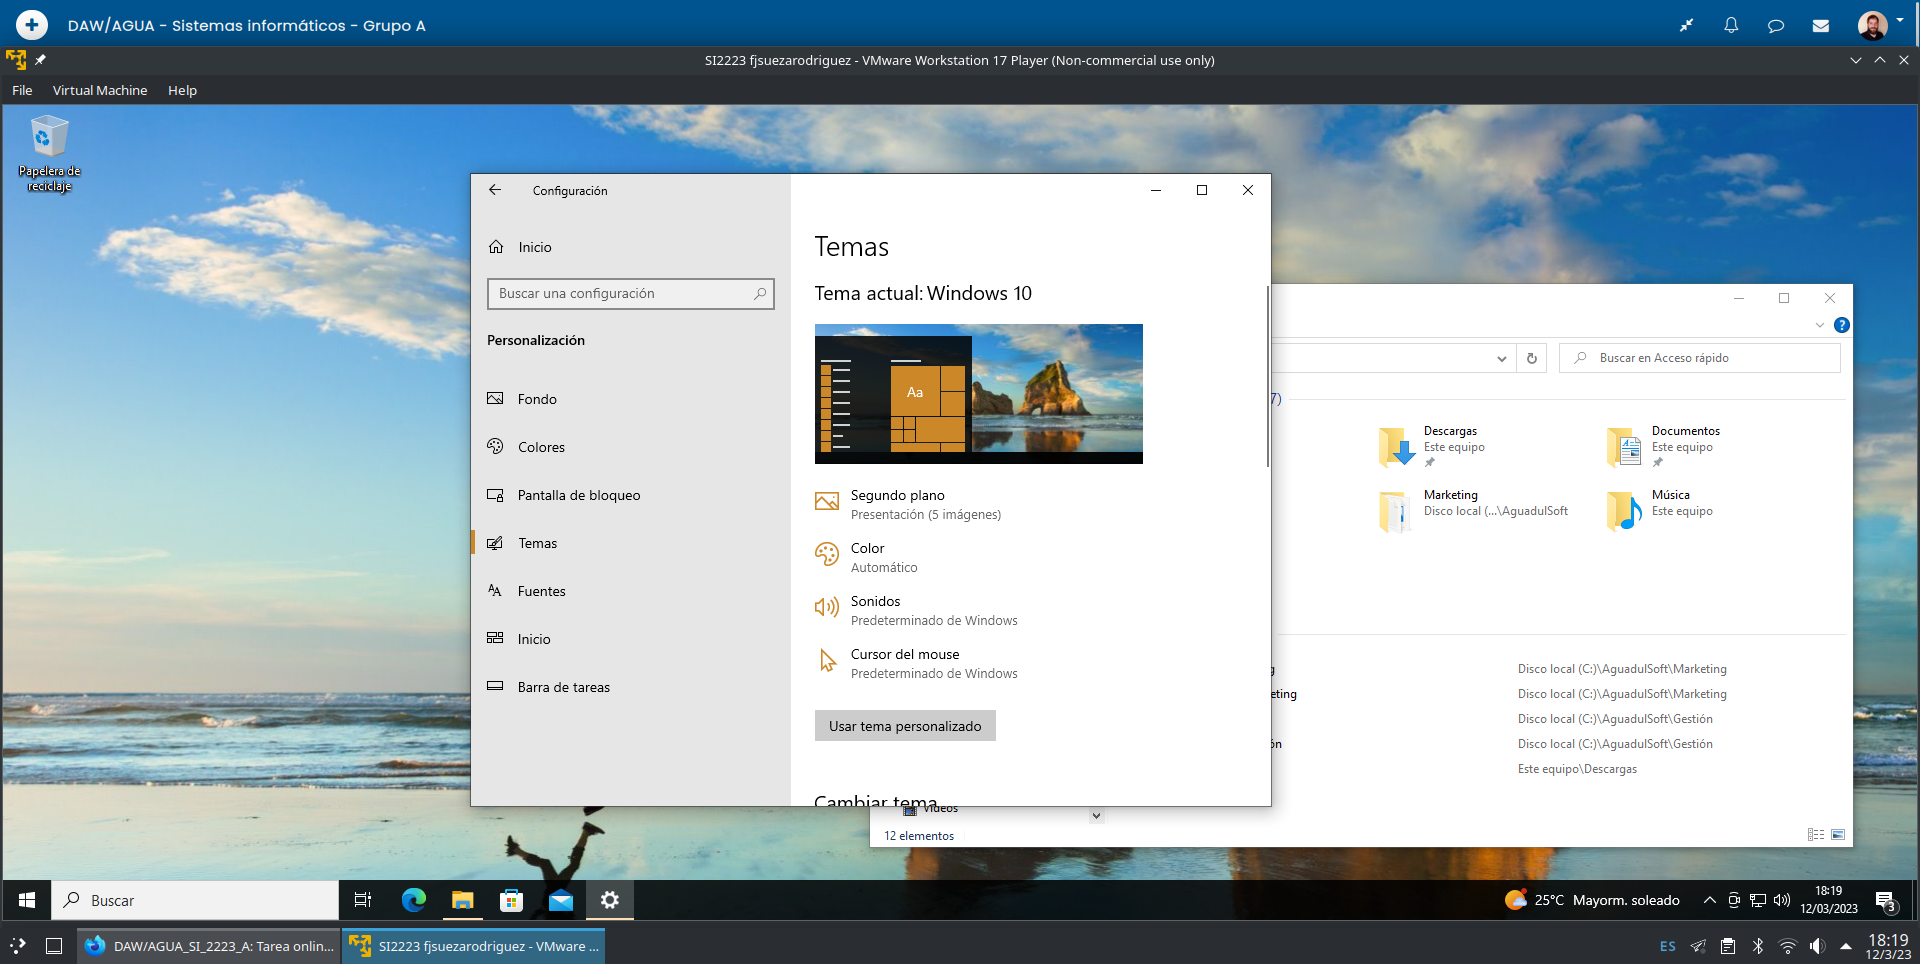
\includegraphics[scale=0.20]{restauracion-3.png}
        \caption{Sistema Restaurado}
    \end{figure}
\end{enumerate}

\subsection{Actividad 10: Copia de Seguridad}
\subsubsection{Enunciado}
Para poder realizar copias de seguridad de los archivos necesitas un disco distinto al de la partición donde se aloja Windows. Debes crear un nuevo disco virtual, siempre con la MV apagada. Añade un nuevo disco duro al conector sata desde la configuración de Almacenamiento y asígnale unos 10 GB con reserva dinámica de espacio.

Cuando inicies la MV el sistema aún no reconocerá el disco (hay que montarlo), tienes que usar la herramienta de administración de discos y crear un volumen simple con el nuevo disco creado y darle formato NTFS. A partir de aquí nuestro sistema ya sí reconocerá el nuevo disco.

Abre \textbf{Copia de Seguridad} para añadir la nueva unidad creada. Configura la copia de seguridad para que además de todas las carpetas asociadas al usuario logueado, incluya en el backup la carpeta \textbf{C:\textbackslash AguadulSoft} de la actividad 1.

La copia de seguridad se realizará cada \textbf{3 horas}, y se mantendrán los archivos durante \textbf{1 año}.

\textbf{Capturas}:

\begin{itemize}
    \item Ventana del Administrador de discos donde se crea el nuevo volumen.
    \item Ventana donde se aprecian las opciones de la Copia de Seguridad, como periodicidad y permanencia de la copia.
\end{itemize}

\subsubsection{Solución}
Como última actividad de esta tarea, vamos a establecer una política de creación de copias de seguridad.

\begin{enumerate}
    \item En primer lugar, hemos usado el \textbf{gestor de volúmenes} para añadir la unidad que hemos creado previamente, una \textbf{unidad de disco duro} de tipo \textbf{SATA} con un tamaño de 10 GB.  En la siguiente imagen podemos ver la unidad, a la que le hemos asignado la \textbf{letra F} y hemos llamado \textbf{backup}, correctamente formateada en el \textbf{gestor de discos}.

    \begin{figure}[H]
        \centering
        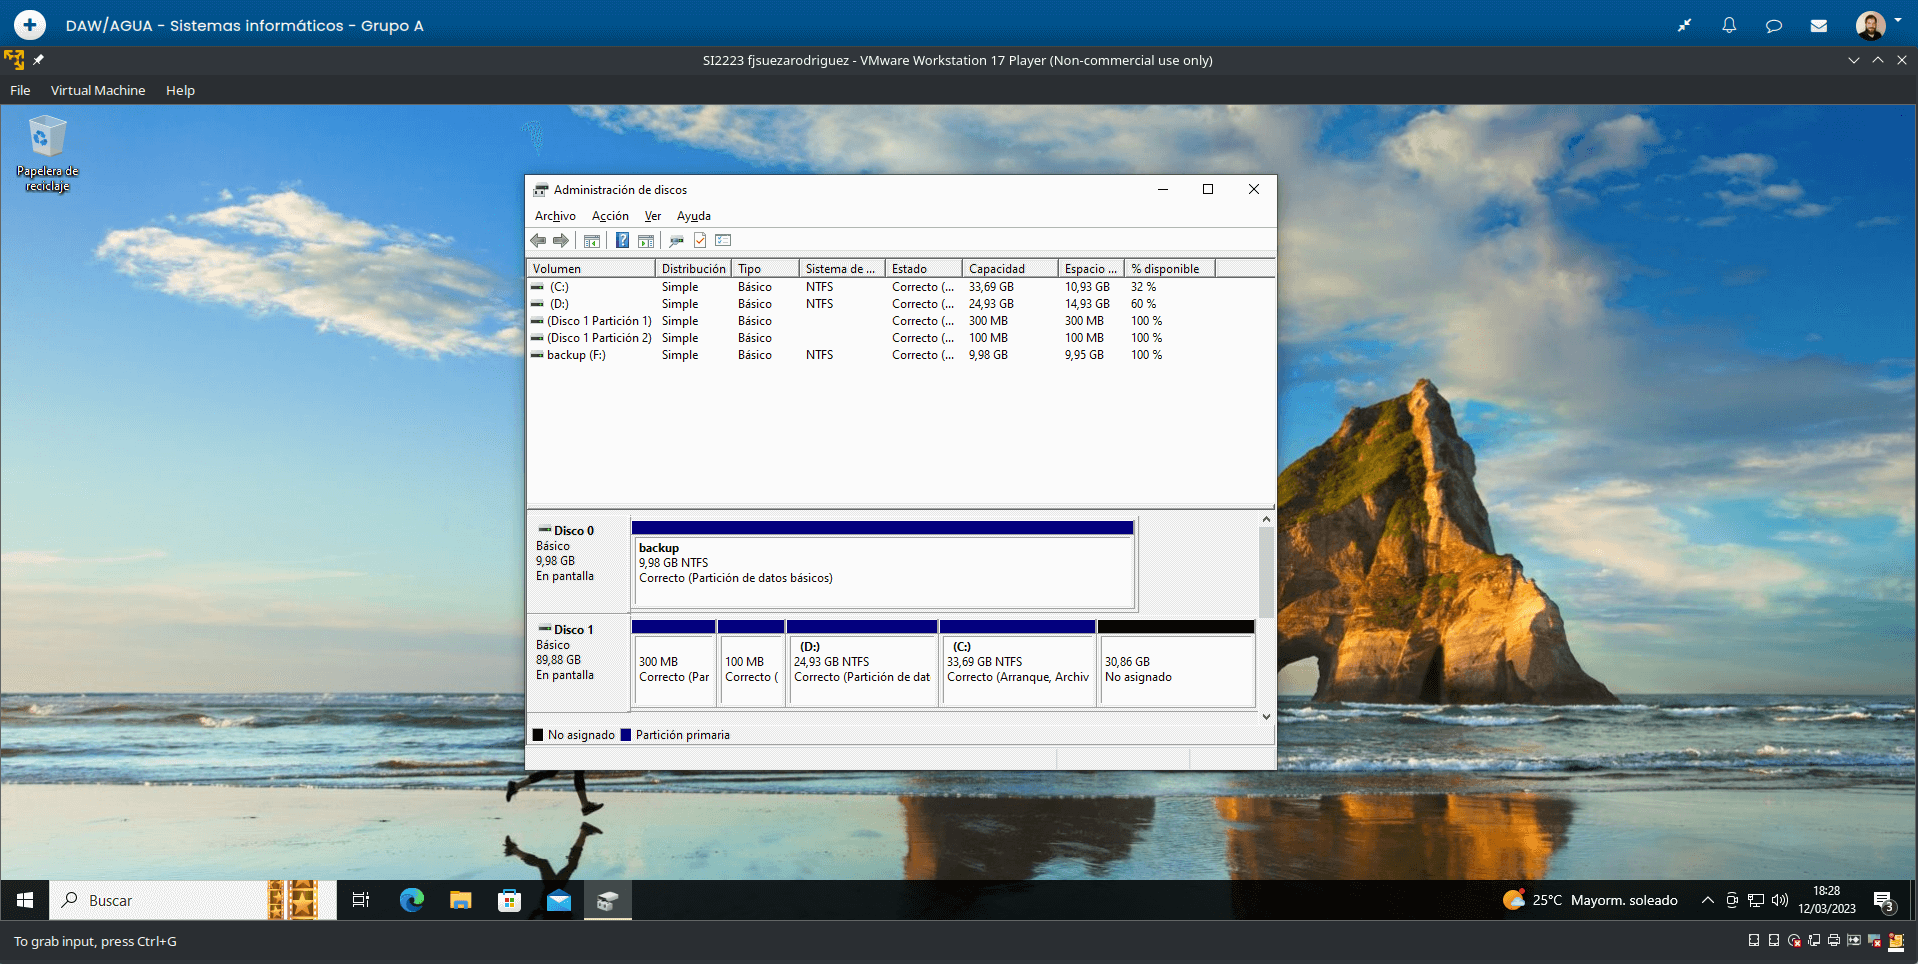
\includegraphics[scale=0.16]{backup-1.png}
        \caption{Nueva unidad formateada en el gestor de discos}
    \end{figure}

    \item A continuación hemos creado la política de copia de seguridad con los parámetros que se nos han indicado. Esto es, realizado una copia de seguridad cada \textbf{3 horas}, con una permanencia de \textbf{1 año} y añadiendo la carpeta \textbf{C:\textbackslash AguadulSoft}. En la siguiente imagen se puede ver la configuración final de las copias de seguridad.

    \begin{figure}[H]
        \centering
        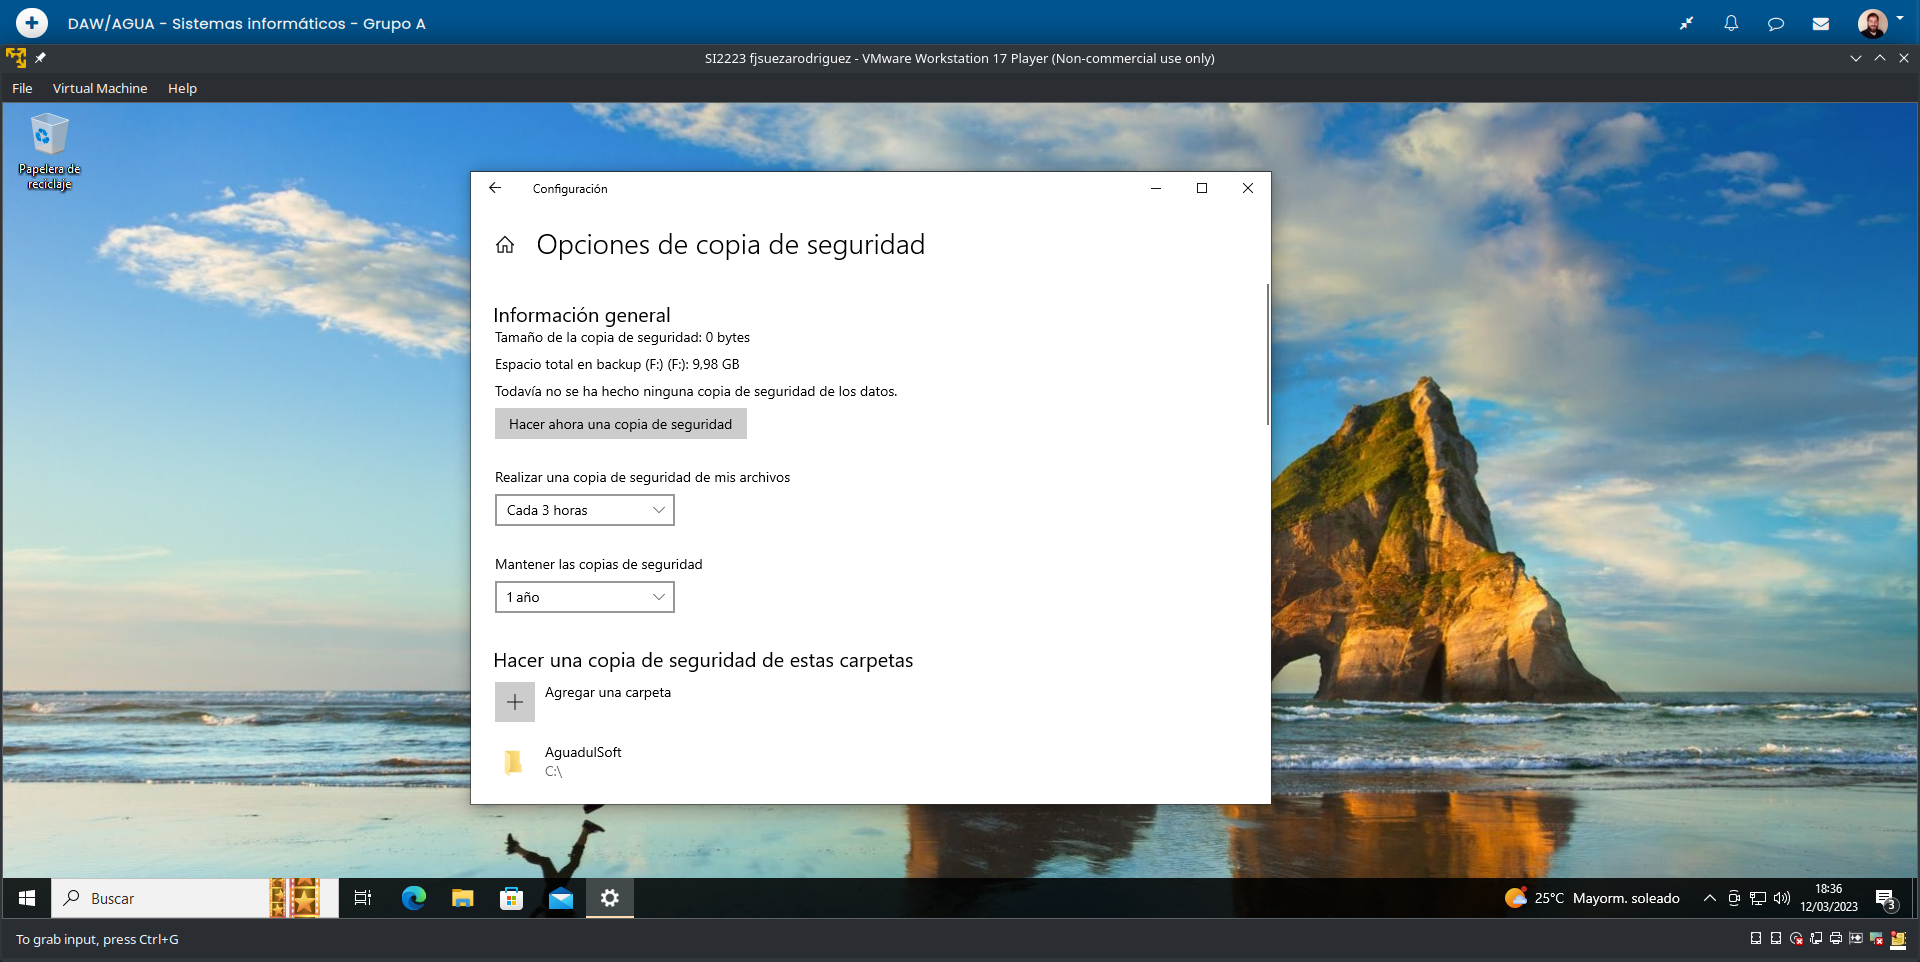
\includegraphics[scale=0.22]{backup-2.png}
        \caption{Configuración de copias de seguridad}
    \end{figure}
\end{enumerate}




% Bibliography

%\newpage
%\bibliography{citas}
%\bibliographystyle{unsrt}

\end{document}